\documentclass[11pt]{amsart}
\usepackage{graphicx}
\usepackage{color}
\usepackage{amssymb}
\usepackage{enumitem}
\usepackage[all,cmtip]{xy}
%\usepackage{url}
\usepackage{hyperref}
%\usepackage[hypertex]{hyperref}
%\usepackage[driverfallback=hypertex]{hyperref}
\usepackage{comment}


\newcommand{\M}{\mathcal{M}}
\newcommand{\A}{\mathbf{A}}
\newcommand{\R}{\mathbb{R}}
\newcommand{\C}{\mathbb{C}}
\newcommand{\T}{\mathbb{T}}
\newcommand{\Z}{\mathbb{Z}}
\newcommand{\N}{\mathbb{N}}
\newcommand{\K}{\mathbb{K}}
\newcommand{\Pp}{\mathbb{P}}
\newcommand{\m}{\mathfrak{m}}

\newcommand{\gl}{l}
\newcommand{\bH}{H}
\newcommand{\vectornorm}[1]{\left\|#1\right\|}
\newcommand{\fat}[1]{\textbf#1}
\newcommand{\cthree}{\textbf c$^3$}
\newcommand{\acs}[1]{#1}
\newcommand{\J}{\acs{J}}
\newcommand{\restrict[3]}{\left. {#2}\right|_{#3}}
\newcommand{\VN}[2]{\vectornorm{#1}^{#2}}
\newcommand{\VNC}[3]{\vectornorm{#1}^{#2}_{#3}}
\newcommand{\VNA}[3]{\vectornorm{\restrict{#1}{#3}}^#2}
\newcommand{\VNCA}[4]{\vectornorm{\restrict{#1}{#4}}^#2_#3}
\newcommand{\VNP}[3]{\vectornorm{#1_{#3}}^{#2}}
\newcommand{\VNCP}[4]{\vectornorm{#1_{#4}}^{#2}_{#3}}
\newcommand{\delbar}[1]{\overline{\partial}_{#1}}
\DeclareMathOperator{\id}{Id}
\DeclareMathOperator{\Log}{Log}
\DeclareMathOperator{\Hess}{Hess}
\DeclareMathOperator{\re}{Re}
\DeclareMathOperator{\val}{val}
\DeclareMathOperator{\can}{can}
\DeclareMathOperator{\area}{Area}
\DeclareMathOperator{\vol}{Vol}
\DeclareMathOperator{\Sec}{Sec}
\DeclareMathOperator{\inj}{inj}
\DeclareMathOperator{\im}{im}
\DeclareMathOperator{\coker}{coker}
\DeclareMathOperator{\Skel}{Skel}
\DeclareMathOperator{\supp}{supp}
\setlist[enumerate,1]{label={(\alph*)}}
\setlist[enumerate,2]{label={(\roman*)}}
%\newtheorem{ex}{Example}
\newcommand{\Yoel}[1]{{\color{red} #1}}

\newtheorem{tm}{Theorem}[section]
\newtheorem*{sa*}{Standing Assumption}
\newtheorem{pr}[tm]{Proposition}
\newtheorem{lm}[tm]{Lemma}
\newtheorem{cy}[tm]{Corollary}
\newtheorem{cm}[tm]{Claim}
\newtheorem{st}{Step}[tm]
\newtheorem*{tm*}{Theorem}
\newtheorem{theorem}{Theorem}
\newtheorem{Qu}[tm]{Question}
\newtheorem*{property}{Robustness property}
\renewcommand*{\thetheorem}{\Alph{theorem}}
\theoremstyle{definition}
\newtheorem{df}[tm]{Definition}




\theoremstyle{remark}
\newtheorem{rem}[tm]{Remark}
\newtheorem{ex}[tm]{Example}
\newtheorem*{exs}{Examples}
\title{Floer theory and reduced cohomology on open manifolds}
\author{Yoel Groman}

\begin{document}

\maketitle
\begin{abstract}
We construct Hamiltonian Floer complexes associated to continuous, and even lower semi-continuous, time dependent exhaustion functions on geometrically bounded symplectic manifolds. We further construct functorial continuation maps associated to monotone homotopies between them, and operations which give rise to a product and unit. The work rests on novel techniques for energy confinement of Floer solutions as well as on methods of Non-Archimedean analysis. The definition for general Hamiltonians utilizes the notion of reduced cohomology familiar from Riemannian geometry, and the continuity properties of Floer cohomology. This gives rise in particular to localized Floer theory. We discuss various functorial properties as well as some applications to existence of periodic orbits and to displaceability.
\end{abstract}

\tableofcontents

\section{Introduction}
Let $(M,\omega)$ be a symplectic manifold. Floer theory is a machine that associates algebraic structures to objects of symplectic geometry on $M$. Over the years, it has come to play central role in all aspects of the field, from mirror symmetry to quantitative symplectic geometry. In this paper we extend the range of applicability of Floer theory, focusing on Hamiltonian Floer theory, to geometrically bounded, or tame, symplectic manifolds. As a byproduct we obtain Floer chain complexes for lower semi-continuous Hamiltonians, a result which is interesting also on closed manifolds.

There is a vast literature employing Hamiltonian Floer theory both on open manifolds and for indicator functions of various sets utilizing ad-hoc constructions or making restrictive assumptions. However, there are numerous settings of central importance which are not covered by the existing literature. To name a few, we have magnetic cotangent bundles and, more generally, twisted Liouville domains, coadjoint orbits of noncompact groups, Hitchin moduli spaces, and complements of an anti-canonical divisor in toric Calabi-Yau varieties. The study of the wrapped Fukaya category in these settings would contribute to our understanding of mirror symmetry, the geometric Langlands program, and to many branches of symplectic topology.

It should be emphasized that while we do not mention the Fukaya category elsewhere in this paper, the difficulties posed by  non-compactness are virtually the same for the Hamiltonian version of Floer theory as for its Lagrangian intersection version. Thus, this paper sets the stage for the study of the (wrapped) Fukaya category on open manifolds such as those mentioned above insofar as one can overcome the usual difficulties already present in the closed case.

The results here provide a unified and flexible framework which incorporates the various constructions in the literature (e.g.,\cite{CielFloerHofer,Viterbo99,Oancea06,Ritter10}), works in full generality, and has transparent symplectic invariance properties. We shall assume familiarity with the basic machinery of Hamiltonian Floer theory and symplectic cohomology such as can be acquired from the first three lectures in \cite{Salamon1999} together with \cite{Oancea04}. For the discussion of the product structure we shall assume also some familiarity with treatments such as \cite{Abouzaid2013} or \cite{Ritter13}. The latter is not necessary for most of the novel ideas in this paper.
\subsection{The main results}
A symplectic manifold $(M,\omega)$ is said to be \textbf{geometrically bounded} if there is an $\omega$-compatible almost complex structure $J$, a constant $C>1$, and  a complete Riemannian metric $g$ with sectional curvature bounded from above and injectivity radius bounded away from $0$ such that
\[
\frac1{C}g(v,v)\leq \omega(v,Jv)\leq Cg(v,v).
\]
Note that the almost complex structure $J$ is \textit{not} part of the data.
Examples include closed symplectic manifolds, cotangent bundles of arbitrary smooth manifolds, manifolds whose end is modeled after the convex half of the symplectization of a compact contact manifold \cite{Sikorav94}, twisted cotangent bundles\cite{CielGinzKer}, and many more. The class of tame symplectic manifolds is closed under products and coverings.

\begin{rem}It should be emphasized that an open symplectic manifold of finite volume, such as the unit ball in $\C^n,$ cannot be endowed with a metric that is at once complete and satisfies the above bounds on sectional curvature and radius of injectivity and thus is \textit{not} geometrically bounded. Floer theory for open finite volume symplectic manifolds, such as Liouville domains, will be discussed, in the context of localized Floer homology, when they are embedded in a geometrically bounded symplectic manifold.
\end{rem}

\textit{Henceforth, $(M,\omega)$ is a semi-positive and geometrically bounded.}  Namely, denoting by $c_1$ the first Chern class of $M$, for any class $A\in\pi_2(M)$ we have
 \[
    3-n\leq c_1(A)<0\qquad\Rightarrow \qquad \omega(A)\leq 0.
 \]
 We hasten to emphasize that this is assumption is made for definiteness only. The methods introduced herein are orthogonal to the usual questions of transversality and can be adapted to any regularization scheme.

Fix a field $R$ and denote by $\Lambda_R$ the universal Novikov field and by $\Lambda_{R,\omega}$ the Novikov field associated with $\omega$. See \S\ref{SecDefHam}. We shall use the notation $\K$ to denote either $\Lambda_R$ or $\Lambda_{R,\omega}$. \textit{In the entire text, $\Lambda_R$ coefficients should be assumed by default whenever the coefficient field is not indicated in the notation.}

The precise statement of the main results requires some preparation. We therefore present first an informal statement which can be seen as the main theorem. In \S\ref{SecIntro2} we give an extended presentation and discussion.
\begin{tm}\label{TmA}
To each proper lower semi-continuous Hamiltonian $H$ on $M$ which is bounded below, one can associate in a natural way a non-Archimedean $\K$-Banach space $\overline{HF}^*(H;\K)$ which specializes to (reduced) Floer cohomology when the latter is well defined. Given $H_1\leq H_2$ there is a functorial map
\[
\overline{HF}^*(H_1;\K)\to\overline{HF}^*(H_2;\K).
\]
Moreover, $\overline{HF}^*(H;\K)$ arises as the reduced cohomology of a certain Banach chain complex which is associated to $H$ up to an appropriate notion of quasi-isomorphism, and which specialize to the Floer chain complex when the latter is well defined.
\end{tm}
Theorem~\ref{TmA} is reformulated more precisely in \S\ref{SecIntro2} as Theorems~\ref{mainTmA} and ~\ref{tmUniExtFl}. Theorem~\ref{mainTmA} introduces a non-empty bidirected and symplectically invariant collection of Floer data, referred to as \textbf{dissipative Floer data}, for which the honest Floer differential and continuation maps are well defined. After introducing the notion of reduced cohomology, Theorem~\ref{tmUniExtFl} then extends the definition of Floer cohomology to the set $\mathcal{H}_{s.c.}$ of lower semi-continuous time dependent exhaustion functions on $M$ using continuity properties of reduced Floer cohomology and an algebraic limiting procedure from~\cite{abouzaidSeidel2010}.


\begin{tm}\label{tmFloerProduct}
\begin{enumerate}
\item
    There is a natural isomorphism
    \begin{equation}\label{eqMorseHomProj}
        \varprojlim_{H\in\mathcal{H}_{s.c}}\overline{HF}^*(H;\K)=H^*(M;\K).
    \end{equation}
\item There is a continuous norm-decreasing bilinear map
\begin{equation}\label{EqSHProd}
*:\overline{HF}^*(H_1;\K)\hat{\otimes}\overline{HF}^*(H_2;\K)\to \overline{HF}^*(H_1+H_2;\K),
\end{equation}
induced by the pair of pants product. It commutes with continuation maps and is associative and super-commutative. The unit of $H^*(M;\K)$ acts as a unit via the isomorphism \eqref{eqMorseHomProj}.
\end{enumerate}
\end{tm}
The proof of Theorem~\ref{tmFloerProduct} is carried out in \S\ref{subsecFloerProd}. Essentially the same proof can be used to construct operations associated with any family of nodal Riemann surfaces and parametrized Floer data. Moreover, it is possible to carry out a Lagrangian intersection variant of the results of this paper. Thus, the TQFT structure presented for the case of Liouville domains in \cite{Ritter13} can be transferred in its entirety to the present setting.

In the rest of this introduction we will use Theorems~\ref{TmA} and~\ref{tmFloerProduct} to construct symplectic cohomology rings and discuss some of their functorial properties and applications. One of the main lessons is that there are two different notions of symplectic cohomology associated with two different topologies one can consider on the direct limit of a sequence of Banach chain complexes. The locally convex topology gives rise to global invariants and can be thought to correspond under mirror symmetry to the ring of algebraic poly-vector fields. The Banach topology gives rise to local invariants and corresponds under mirror symmetry to locally defined analytic poly-vector fields. This distinction appears to have been masked to a large extent in the literature so far due to the emphasis on Liouville domains with trivially valued coefficient fields where various different invariants coincide.  A similar observation is made in a recent paper by S. Venkatesh\cite{Venkatesh2017}.
\subsection{Localized Floer theory}
Let $K\subset M$ be a compact set. Let
\[
H_K(x):=\begin{cases} 0, & x\in K,\\ \infty, & x\in M\setminus K.\end{cases}
\]
The \textbf{localized symplectic cohomology} at $K$ is defined by
\[
SH^*(M|K;\K):=\overline{HF}^*(H_K;\K).
\]
The following theorem lists the basic properties of $SH^*(M|K;\K)$ which can be almost readily read off Theorems~\ref{TmA} and~\ref{tmFloerProduct}.
\begin{tm}\label{tmLocFlHoProp}
\begin{enumerate}
\item The map $K\mapsto SH^*(M|K;\K)$ is contravariantly functorial with respect to inclusions.
\item Any symplectomorphism $\psi$ induces an isometry
    \[
    \psi_*:SH^*(M|K;\K)\to SH^*(M|\psi(K);\K).
    \]
\item $SH^*(M|K;\K)$ is a unital $\K$-algebra with respect to $*$.
\item We have a commutative triangle of $\K$-algebras
\[
\xymatrix{
H^*(M;\K)\ar[d]\ar[dr]& \\
SH^*(M|K_2;\K) \ar[r] &SH^*(M|K_1;\K)
}
\]
\item For any $H\in\mathcal{H}$ which is bounded on $K$ we have a continuous map and functorial map
\[
\overline{HF}^*(H;\K)\to SH^*(M|K;\K),
\]
which increases the valuation\footnote{By definition, the valuation is $\val:=\log\|\cdot\|.$} by at most $c=-\sup_KH$.
\end{enumerate}
\end{tm}
The proof of Theorem \ref{tmLocFlHoProp} appears at the end of \S\ref{subsecFloerProd}
\begin{rem}
Suppose $M$ is symplectically a-spherical and $H_K$ can be approximated by Hamiltonians whose periodic orbits have non-negative action. Then the commutative triangle \eqref{eqLocComTri} can be refined to a commutative square
\[
\xymatrix{
H^*(K_2;\K)\ar[d]\ar[r]&H^*(K_1;\K)\ar[d]& \\
SH^*(M|K_2;\K) \ar[r] &SH^*(M|K_1;\K).
}
\]
Combined with \eqref{eqLocLiouvDom} below, this generalizes Viterbo's commutative square for Liouville domains\cite{Viterbo99}.
\end{rem}
\begin{rem}
We comment on the name localized symplectic cohomology. First suppose the boundary of $K$ is stable Hamiltonian. Then it can be shown that elements of $SH^*(M|K)$ are represented by linear combinations of constant periodic orbits inside $K$ and the Reeb orbits of $\partial K$. More generally, these can be represented by, in addition to constants, periodic orbits lying arbitrarily close to $\partial K$. For a particular manifestation of this, see Theorem~\ref{lmNearbyEx} below. Thus $SH^*(M|K)$ can be thought of as symplectic cohomology relative to the complement of $K$. That is, as localized at $K$.
\end{rem}


\begin{tm}\label{lmNearbyEx}
Let $H$ be a smooth Hamiltonian such that $H^{-1}(0)=\partial K$.
\begin{enumerate}

\item
Suppose $\alpha$ is a non-trivial free homotopy class and let $SH^{*,\alpha}(M|K;\K)$ denote the localized symplectic cohomology generated by periodic orbits in the class $\alpha$. Suppose $SH^{*,\alpha}(M|K;\K)\neq 0$. Then there is a sequence $a_n>0$ converging to $0$ such that $H^{-1}(a_n)$ has a periodic orbit representing $\alpha$.
\item\label{lmNearbyExPartB}
Suppose $c_1(M)=0$. If $SH^*(M|K;\K)\neq H^*(K;\K)$ then there is a sequence $a_n>0$ converging to $0$ such that $H^{-1}(a_n)$ has a contractible periodic orbit.
\end{enumerate}
\end{tm}
Theorem \ref{lmNearbyEx} is proven in \S \ref{subsecNearby}.
\begin{comment}
\begin{tm}\label{tmCircleAcVan}
Suppose $c_1(M)=0$ and that $M$ carries a circle action generated by a Hamiltonian $H$ which is proper and bounded from below. Then for any sublevel set $U$ of $H$, we have that
\[
SH^*(U;\K)=0.
\]
\end{tm}
Combining theorems \ref{lmNearbyEx}\ref{lmNearbyExPartB} and \ref{tmCircleAcVan} we obtain
\begin{cy}[\textbf{Obstruction to circle action}]
Suppose $c_1(M)=0$. If there exists a Hamiltonian $H$ which has no contractible periodic orbits outside some compact set then $M$ does not carry a Hamiltonian circle action generated by a Hamiltonian which is proper and bounded from below.
\end{cy}
In \cite{a,b} numerous examples are given of magnetic cotangent bundles having no contractible periodic orbits on levels beyond the Mane critical value.
\end{comment}
Some applications of local Floer cohomology to embedding and displaceability problems are given in \S \ref{subsecLiouIntro} below.

We conclude with some comments on the relation of these groups with similar work of others.
\begin{enumerate}[wide, labelwidth=!, labelindent=10pt]
\item When $M$ is symplectically aspherical and $K$ is the closure of an open set $U$, the  groups $SH^*_{[a,b)}(M|K)$ coincide with the corresponding symplectic cohomology groups of $U$ as defined in \cite{CielFloerHofer} using Hamiltonians which are constant at infinity.
\item In \cite{Venkatesh2017} the notion of completed symplectic cohomology is introduced and studied for Liouville cobordisms $\mathcal{W}$ inside monotone symplectic manifolds. The computations in \cite{Venkatesh2017} show that the local symplectic cohomology groups depend non trivially on $K$. The choice of Floer data in \cite{Venkatesh2017} is such that the Floer chain complexes have finite boundary depth. In particular ordinary and reduced Floer cohomology coincide for these Floer data.  A consequence of Theorem~\ref{tmUniExtFl} is that the invariant of \cite{Venkatesh2017} is the local Floer cohomology as defined here.
\item In his as yet unpublished thesis, U. Varolgunes studies an invariant which coincides with local symplectic cohomology as defined here on the common domain of definition. He proves numerous results, in particular for the case of invariant sets in integrable systems.
\end{enumerate}
\subsection{Symplectic cohomology}
\textit{In this subsection we work exclusively with $\Lambda_R$ coefficients}. We do this to avoid working over trivially valued fields for which some basic theorems in non-Archimedean analysis fail to hold.

\begin{df}
Let $\mathcal{H}_0\subset\mathcal{H}_{s.c.}$ be a semigroup with respect to pointwise addition. The symplectic cohomology ring $SH^*(M;\mathcal{H}_0,\Lambda_R)$ is defined by
\[
SH^*(M;\mathcal{H}_0,\Lambda_R):=\varinjlim_{H\in\mathcal{H}_0}\overline{HF}^*(H;\Lambda_R),
\]
with the product induced by $*$. $SH^*(M;\mathcal{H}_0)$ is a non-Archimedean locally convex topological vector space over $\Lambda_R$. We denote by $\widehat{SH}^*(M;\mathcal{H}_0)$ its Hausdorff completion. For a more detailed discussion, see \S\ref{SecSHuniv}.
\end{df}


Denote by $\mathcal{H}\subset\mathcal{H}_{s.c.}$ the set of continuous time dependent exhaustions. For any geometrically bounded symplectic manifold we obtain a symplectic invariant.
\begin{df}
The \textbf{universal symplectic cohomology} is defined by
\[
\widehat{SH}^*_{univ}(M):=\widehat{SH}^*(M;\mathcal{H}).
\]
\end{df}
\begin{rem}
As discussed in Remark~\ref{rmLocConvDet}, there is generally no guarantee that $\widehat{SH}_{univ}$ is well behaved as a topological vector space. Namely, it may be non-metrizable. Better behaved topological vector spaces are obtained when one considers semi-groups $\mathcal{H}_0$ with appropriate restrictions on the growth at infinity. Such semi-groups play a role in numerous settings considered in the literature \cite{Viterbo99,Oancea06,Ritter10}. In forthcoming papers this will be discussed in relation to SYZ mirror symmetry on open manifolds and to magnetic cotangent bundles.
\end{rem}
We list some applications of $\widehat{SH}^*_{univ}(M)$.

Let $(M,\omega)$ be a compact symplectic manifold and let $\psi:M\to M$ be a symplectomorphism. Denote by $\tilde{M}_\psi$ the associated symplectic mapping torus. See \S\ref{subSecMappingTorus} for the definition. Denote by $HF^*(M,\psi)$ the fixed point Floer homology of $\psi$ as introduced in \cite{DS94}. The following theorem allows to distinguish mapping tori by fixed point Floer homology.

\begin{tm}[Cf.  \cite{Fabert10}]\label{tmMappFloFixed}
We have $\widehat{SH}^*_{univ}(\tilde{M}_\psi)\simeq\hat{\oplus
}_{k\in\Z }HF^*(M,\psi^k).$ Here the right hand side is the completion with respect to the $\sup$ norm and $\simeq$ denotes isomorphism of the underlying topological vector space. In particular, let $\psi_i:M\to M$ be a symplectomorphism for $i=0,1$. Suppose there exists a symplectomorphism
\[
 \phi:\tilde{M}_{\psi_1}\to\tilde{M}_{\psi_2}.
 \]
 Then $\phi$ induces an isomorphism $HF^*(M,\psi_1)=HF^*(M,\psi_2)$.
\end{tm}
Theorem \ref{tmMappFloFixed} is proven in \S \ref{subSecMappingTorus}.


\begin{tm}[\textbf{Kunneth formula}]\label{tmKunneth}
Let $M_1$ and $M_2$ be tame symplectic manifolds. Then
\begin{equation}\label{eqKunnethSH}
\widehat{SH}_{univ}^*(M_1\times M_2)=\widehat{SH}_{univ}^*(M_1)\hat{\otimes}_\epsilon\widehat{SH}_{univ}^*(M_2).
\end{equation}
Here the tensor product is the injective tensor product in the category of complete locally convex non-Archimedean topological vector spaces.
\end{tm}
Theorem \ref{tmKunneth} is proven in \S \ref{subsecKunnethSH}.
\begin{tm}[\textbf{Nearby existence }]\label{tmNearbyEx0}
\begin{enumerate}
\item\label{NearbyEx1} Suppose that $c_1(M)=0$ and $\widehat{SH}_{univ}^*(M)=0$. Then for any Hamiltonian $H:M\to\R$ which is proper and bounded from below, the subset of levels containing a contractible periodic orbit is dense in $H(M)\subset\R$.
\item\label{NearbyEx2} Let $\alpha\neq 1\in\pi_1(M)$. Suppose $\widehat{SH}^{*,\alpha}(M)\neq\{0\}$. Then there is a compact $K\subset M$ such that for any smooth proper and bounded below $H:M\to\R$ and any $a\in \R$ for which  $H(K)\subset(-\infty,a]$ the set of $x\in[a,\infty)$ for which $H^{-1}(x)$ has a periodic orbit representing $\alpha$ is dense in $[a,\infty)$.
\end{enumerate}
\end{tm}
Theorem \ref{tmNearbyEx0} is proven in \S\ref{subsecNearby}.
\begin{rem}
Examples satisfying the hypotheses of the first part of Theorem \ref{tmNearbyEx0} are complete toric varieties $M$ such that $c_1(M)=0$. This follows from the vanishing criterion of Theorem \ref{tmVanishing}. See Example \ref{exTCy}. There are manifolds in this class of examples which unlike $\C$ contain non-displaceable sets. Examples are the canonical bundles over $\Pp^2$ and over $\Pp^1\times \Pp^1$. By the Kunneth formula, the product of such a manifold with any geometrically bounded symplectic manifold of vanishing Chern class will again satisfy the hypothesis.

An example of an $M$ and $\alpha$ satisfying the hypotheses the second part of Theorem \ref{tmNearbyEx0} is given by the cotangent bundle of the torus and any non-trivial homotopy class $\alpha$. This can be deduced from Theorems \ref{tmMappFloFixed} and \ref{tmKunneth}. From this  we obtain many examples by taking the product with an arbitrary compact manifold or with a geometrically bounded one for which symplectic cohomology does not vanish, and considering homotopy classes pulled from the cotangent factor.
\end{rem}

We can also use the methods of this paper to produce periodic orbits with prescribed action. Namely, for a dissipative Hamiltonian $H$ call a class $a\in \overline{HF}^*(H)$ \textbf{essential} if it maps to a non-zero class in $\widehat{SH}_{univ}^*(M)$. Suppose $M$ is symplectically a-spherical. If $H_1\leq H_2$ are dissipative then for any essential class $a$ in $HF^*(H_1)$ there is a periodic orbit of $H_2$  in the same homotopy class with action bounded by $\val(a)$. Indeed, the map $HF^*(H_1)\to \widehat{SH}^*_{univ}(M)$  factors through $HF^*(H_2)$ by the continuation map which is action decreasing.

\begin{ex}
On a Liouville domain, for any function $H$ which is convex at infinity, all non-zero classes in $HF^*(H)$ are essential. This follows from Theorem \ref{tmVitrUniv} below. The same holds for the product of a Liouville domain with a compact a spherical manifold. These claims require working over $R$ instead of over $\Lambda_R$, but this is not problematic in this restricted setting since the action spectrum is bounded below and so the topology is discrete.
\end{ex}



 \begin{comment}
\begin{df}
Let $\mathcal{H}_0\subset\mathcal{H}$ be a directed system which is closed with respect to taking finite sums. Define
\[
{SH}^*_{\mathcal{H}_0}(M):=\overline{\varinjlim}_{H\in\mathcal{H}_0}\overline{HF}^*(H).
\]
Here, the over line denotes a reduced direct limit which is the direct limit is taken in the category of complete locally convex non-Archimedean vector spaces. For details see \S\ref{SecSHuniv}.
\end{df}
\begin{rem}
We should point out that the reduced direct limit is not a standard construction in the literature. In Lemma~\ref{lmFinDimLim} we show that when the direct limit is taken over a sequence of finite dimensional spaces, a common condition, the reduced direct limit coincides with the ordinary direct limit.
\end{rem}
\end{comment}
\begin{comment}

\begin{rem}
When $\mathcal{H}_0$ admits a cofinal monotone sequence $\{H_i\}$, $\overline{SH}^*_{\mathcal{H}_0}(M)$ can be computed via the telescope construction as the reduced cohomology of a certain chain complex which we denote by $SC^*(\{H_i\})$ obtained from a direct sum of the Banach complexes $CF^*(H_i)$ considered with the locally convex topology.  The same complexes can be used to form Banach complexes by completing with respect to the $\sup$ norm. The resulting groups will generally be completely different. As a rule, if we take the Banach topology on $SC^*(\{H_i\})$ we obtain the Floer cohomology $\overline{HF}^*(\sup_iH_i)$ as defined in the previous section. The locally convex topology gives rise to an invariant which is much less sensitive to the Floer data used to compute it and may thus be thought to reflect more global aspects of symplectic topology. This observation has been made recently in \cite{Venkatesh2017}.
\end{rem}
\end{comment}



\subsection{Liouville domains and displaceability}\label{subsecLiouIntro}
\begin{comment}
We make a few comments about how various constructions specific to Liouville domains fit into the picture just sketched. It turns out, perhaps surprisingly, that it matters very much whether we work over a trivially valued field $R$ or over a Novikov field which for definiteness we take as $\Lambda_R$.
\end{comment}
Let $M$ be the completion of a Liouville domain $U$. Denote by $SH^*_{Viterbo}(U;\K)$ the symplectic cohomology as defined in \cite{Viterbo99} by taking a limit over all $(H,J)$ where $H$ is linear at infinity and $J$ is of contact type.  See \S\ref{subSecLiouville} for notation and definitions. Denote by $\mathcal{L}\subset\mathcal{H}$ the directed set of Hamiltonians which are linear at infinity. We have
\[
SH^*_{Viterbo}(U;\K)=SH^*(M;\mathcal{L},\K),
\]
and therefore a natural map
\[
f:SH^*_{Viterbo}(U;\K)\to \widehat{SH}^*_{univ}(M;\K).
\]
We prove in Theorem~\ref{VitUnivEmb} below
\begin{tm}\label{tmVitrUniv}
The map $f$ is an isomorphism over $\Lambda_{R,\omega}=R$ coefficients.
\end{tm}
\begin{cy}
For a Liouville manifold $M$ of finite type, $SH_{Viterbo}^*(M;R)$ is independent of the choice of primitive of the symplectic form.
\end{cy}

\begin{comment}
A similar setting is that of negative symplectic fibrations over compact aspherical manifolds considered by \cite{Oancea07}. It is no hard to show that the same holds. A corollary is that these constructions of symplectic cohomology are truly symplectic invariants, independent of the contact structure at infinity and the fibration.
\end{comment}
\begin{rem}
Theorem \ref{tmVitrUniv} can generally \textit{not} be expected to be true over a non-trivially valued field. See Remark \ref{rmTrivNonTriv} for an explanation on this point.
\end{rem}
It is also not hard to show that for any Liouville sub-domain $V\subset M$ we have a natural isomorphism of vector spaces
\begin{equation}\label{eqLocLiouvDom}
SH^*(M|V;R)=SH^*_{Viterbo}(V;R).
\end{equation}
Note however that the left hand side of \eqref{eqLocLiouvDom} is naturally a normed vector space while the right hand side is not. The equation will thus cease to be  true over a non-trivially valued field. The generalization of \eqref{eqLocLiouvDom} for the non-trivially valued case is the following excision principle
\begin{equation}\label{eqLocLiouvDomNT}
SH^*(M|V;\Lambda_R)=SH^*(\hat{V}|V;\Lambda_R)
\end{equation}
whenever $M$ is a Liouville manifold and $V$ is a Liouville subdomain with $\hat{V}$ its completion. This follows by the no escape Lemma near the concave boundary of $M\setminus V$. See \cite{Ritter13}. We now formulate a theorem showing that this independence of the ambient manifold holds under more general conditions for skeleta of Liouville domains. In the following, we denote by $SH^{*,0}(M|V)$ the subgroup consisting of periodic orbits that are contractible in $M$. The proofs of the following Theorems are given in \S \ref{subSecLiouville}.
\begin{tm}\label{tmSkellVitFunc}
Let $M$ be symplectically a-spherical and let $U$ be a Liouville domain. Let $i:U\to M$ be an embedding with the property that $i_*H_1(U;\R)\to H_1(M;\R)$ is injective. Then
\[
SH^{*,0}(M|\Skel(U);\mathbb{K})=SH^{*,0}(U|\Skel(U);\mathbb{K}).
\]
\end{tm}
\begin{rem}
The restriction to contractible periodic orbits in Theorem \ref{tmSkellVitFunc} can be removed by adding the assumption that $M$ is symplectically a-toroidal.
\end{rem}
Theorem \ref{tmSkellVitFunc} implies
\begin{tm}\label{tmLiouSubNondisp}
Let $U$ and $M$ be as in Theorem \ref{tmSkellVitFunc} and suppose
\begin{equation}\label{tmNonDispNeq0}
SH^*_{Viterbo}(U)\neq 0.
\end{equation}
Then $\Skel(U)$ is not displaceable.  In particular, no simply connected Liouville domain satisfying~\eqref{tmNonDispNeq0} can be embedded in the product $\C\times M$ where $M$ is symplectically a-spherical and geometrically bounded.
\end{tm}

Taking $U$ the cotangent disc bundle, this is a well known theorem by Gromov. Namely, $\C^n$ contains no simply connected Lagrangians. The particular case $M=\hat{U}$, the completion of $U$, is a theorem by \cite{kang2014}. We remark that Theorem \ref{tmLiouSubNondisp} follows from Theorem \ref{tmSkellVitFunc} by a general vanishing principle for the localized Floer cohomology of a displaceable set. We prove this for $M$ aspherical. In a forthcoming work by U. Varolgunes this is proven without the asphericity assumption. Note however that the asphericity assumption in the last two theorems cannot be removed. Indeed, the anti-diagonal in $\C P^n\times\C P^n$ is simply connected and displaceable. However, there are quantitative counterparts which should hold assuming essentially only tameness.
\begin{tm}\label{tmEpsLiouEmb}
Let $M$ be semipositive and let $U\hookrightarrow M$ be a Liouville domain. Then there is a $\delta>0$ for which $SH^{*,0}_{Viterbo}(U;R)$ embeds into $SH^{*,0}_{[0,\delta)}(M|\Skel(U);\K)$ with valuation $0$ as an $R$-subspace.
\end{tm}

\begin{tm}\label{tmPosDis}
Let $M$ be aspherical and let $U\hookrightarrow M$ be a Liouville domain satisfying $SH^*_{Viterbo}(U)\neq 0$. Then $\Skel(U)$ has positive displacement energy.
\end{tm}

\begin{rem}
It should not be hard to remove the asphericity assumption. Once this is done and taking $U$ to be the cotangent disk bundle we recover a classical theorem by Chekanov \cite{Chekanov1998} stating that Lagrangian submanifolds have positive displacement energy.
\end{rem}

\subsection{Organization of the paper}
The paper is organized as follows. \S\ref{SecIntro2} formulates Theorems~\ref{mainTmA} and \ref{tmUniExtFl} which constitute a more formal and detailed statement of Theorem \ref{TmA}. Section \S\ref{secOvrview} provides an overview of the techniques going into the proof of Theorem~\ref{mainTmA}. Sections \S\ref{Sec1} through \S\ref{Sec5} are devoted to constructing Floer data with appropriate compactness properties required for the proof of Theorem~\ref{mainTmA}. The latter is carried out in \S\ref{Sec6}. In \S\ref{SecHamFloer} we prove Theorems~\ref{tmUniExtFl} and~\ref{tmFloerProduct} and discuss topological aspects of the direct limit in the definition of symplectic cohomology. In \S\ref{Sec7} we carry out the proofs of the properties and applications mentioned in the introduction.
\subsection{Acknowledgements}
This work subsumes part of the author's PhD thesis carried out in the Hebrew University of Jerusalem.  The author is grateful to the Azrieli foundation for granting him an Azrieli fellowship at that time.

Various stages of the work were carried out at the math departments of Hebrew University of Jerusalem, the ETH of Zurich, and Columbia University. They were supported by the ERC Starting Grant 337560, ISF Grant 1747/13, Swiss National
Science Foundation (grant number 200021$\_$156000) and the Simons Foundation/SFARI ($\#$385571,M.A.).

The author would like to thank his thesis advisor Jake P. Solomon for his guidance throughout his graduate work and for a great number of discussions and suggestions. The author is grateful to Mohammed Abouzaid for suggesting some key ideas and to Paul Biran, Lev Buhovski, Sheel Ganatra, Alex Oancea, Dietmar Salamon, Ran Tessler, Amitai Zernik, Umut Varolgunes and Sara Venkatesh, for useful input and enlightening discussions.
\section{The main results: a detailed statement}\label{SecIntro2}
For a symplectic manifold $(M,\omega)$, denote by $\mathcal{J}(M,\omega)$ the set of $\omega$-compatible almost complex structures on $M$. Let
\[
    \mathcal{F} \subset C^{\infty}(S^1\times M)\times C^{\infty}(S^1,\mathcal{J}(M,\omega))
\]
denote the set of Floer data $(H,J)$ such that $H$ is proper and bounded from below, the  Hamiltonian flow of $H$ is defined for all time, and the metric $g_{J_t}:=\omega(\cdot,J_t\cdot)$ is complete for any $t\in S^1$. The set $\mathcal{F}$ is partially ordered by the relation
\[
(H_0,J_0)\leq (H_1, J_1)\iff H_0(x)\leq H_1(x),\forall x\in M.
\]

\begin{comment}
Fix a field $R$ and denote by  $\Lambda_R$ the universal Novikov field. See Section~\ref{SecDefHam}. We shall use the notation $\mathbb{F}$ to denote either $R$ or $\Lambda_R$.
\end{comment}
\begin{tm}\label{mainTmA}
There exists a bi-directed system $\mathcal{F}_d\subset\mathcal{F}$ of Floer data which satisfies the following:
\begin{enumerate}
\item
$\mathcal{F}_d$ is open in $C^1\times C^0$ with respect to the uniform norm induced in a neighborhood of $(H,J)$ by the metric $g_J$.
\item
$\mathcal{F}_d$ is symplectically invariant under the action \[
\psi\cdot(H,J)\mapsto (H\circ\psi,\psi^*J),
\]
for $\psi$ \textit{any} symplectomorphism.
\item \label{mainTmA:itC}For each geometrically bounded almost complex structure $J$, $\mathcal{F}_d$ contains all pairs $(H,J)$ such that $H$ is Lipschitz with sufficiently small Lipschitz constant with respect to $g_J$.
\item A generic $(H,J)\in\mathcal{F}_d$ gives rise to a well defined Floer chain complex $CF^*(H,J;\K)$ generated over $R$ by a Novikov covering of the periodic orbits of $H$ and whose differential is defined by counting connecting Floer trajectories.
\item \label{MainTmAPartE}With any pair $F_1=(H_1,J_1)\leq F_2=(H_2,J_2)$ there is associated in a symplectically equivariant manner a contractible open set of monotone homotopies $\mathcal{F}_d(F_1,F_2)$ which satisfies the following. A generic element $\mathfrak{H}\in \mathcal{F}_d(F_1,F_2)$ gives rise to a well defined chain map
    \[
    CF^*(H_1,J_1)\to CF^*(H_2,J_2).
    \]
    The induced map on homology is independent of the choice of $\mathfrak{H}$ and is functorial with respect to $\leq$.
    \end{enumerate}
\end{tm}
Theorem \ref{mainTmA} is proven at the end of \S\ref{SecDefHam} after a fuller chain level statement is given.

We will refer to the elements of $\mathcal{F}_d$ as \textbf{dissipative} Floer data. We will denote by $\mathcal{H}_d\subset C^{\infty}(S^1\times M)$ the projection of $\mathcal{F}_d$ on the first factor and refer to the elements of $\mathcal{H}_d$ as \textbf{dissipative} Hamiltonians. In the next section, we give a detailed overview of the techniques used to define the directed system $\mathcal{F}_d$. The construction of $\mathcal{F}_d$ spans Sections~\ref{Sec1} through~\ref{Sec5}. We discuss a number of naturally occurring examples of dissipative Floer data throughout the paper, but in general verifying this for a given Floer datum may be non-trivial. Theorem~\ref{tmUniExtFl} which is the second of the two main theorems of this paper serves to a large degree to overcome this difficulty. Namely we will show how to extend the definition of Floer chain complexes to arbitrary exhaustion Hamiltonians in a way that allows putting the detailed constructions of Theorem \ref{mainTmA} into a black box for most theoretical purposes. We emphasize though that the question of whether a given Hamiltonian is dissipative remains important in many instances when studying specific examples.

Before proceeding  we make a few comments.
\begin{enumerate}[wide, labelwidth=!, labelindent=10pt]
\item The Hamiltonians for which Floer cohomology is well defined according to Theorem~\ref{mainTmA} are proper. In particular, they are not compactly supported. To the authors' knowledge, geometric boundedness has been used so far, e.g, in \cite{CielFloerHofer}, only for compactly supported Hamiltonians. The condition on the support requires one to work on symplectically a-spherical manifolds and use the action filtration to avoid the highly degenerate constant periodic orbits. Theorem~\ref{mainTmA} has no such limitations. Moreover, from the point of view of both mirror symmetry and dynamics, it is often important to work with Hamiltonians of sufficiently fast growth at infinity. Floer cohomology for certain types of proper Hamiltonians has hitherto been defined mostly in the setting of manifolds whose end is modeled on the positive half of the symplectization of a contact manifold \cite{Viterbo99,Ritter10}\footnote{We point out the notable exception of \cite{AbondandoloSchwartz06} which uses a method tailored to the specific case of the cotangent bundle.}. But there are many interesting settings where one does not have recourse to such a structure at infinity. Among these are SYZ mirror symmetry and twisted cotangent bundles, both settings to be investigated in forthcoming papers.
\item Part \ref{MainTmAPartE} of Theorem \ref{mainTmA} is one of the main contributions of this paper. It employs the notion of intermittent-boundedness introduced in Definition~\ref{dfIntBounded} below and the method of zig-zag homotopies in the proof of Theorem \ref{tmWeakTameCont} to circumvent the difficult question of the connectedness of the space of geometrically bounded $\omega$-tame almost complex structures on a given symplectic manifold $(M,\omega)$. See remark \ref{rmGeoBCont}. This method is used also in Theorem~\ref{TmSympInvGWSH} below to show that in numerous contexts where invariants on open manifolds are defined using geometrically bounded almost complex structures $J$, the resulting invariants do not depend on the choice of such a $J$.
\end{enumerate}
\subsection{Reduced Floer cohomology}\label{subsecRedFlCo}
To state our next result we need to introduce the notion of reduced cohomology familiar from Riemannian geometry in the context of  $L^p$-cohomology. Namely, the complexes $CF^*(H,J)$ can be considered as non-Archimedean Banach spaces over $\Lambda_R$ with norm given by $\|\cdot\|:=e^{\val(\cdot)}$. On an open manifold, $CF^*(H,J)$ will typically not be finitely generated over the Novikov ring. This means that the differential can generally not be expected to be a closed operator.
\begin{df}
Let $(C^*,d)$ be a topological complex. The \textbf{reduced cohomology} of $C^*$ is
\[
\overline{H}^*(C^*,d):=\widehat{\ker {d^{*}}}/\overline{\im d^{*-1}},
\]
with the hat denoting completion and the over-line denoting the closure inside the completion. For a dissipative $H$, we denote the reduced Floer cohomology by $\overline{HF}^*(H)$\footnote{We suppress $J$ in the notation since the homology is independent of $J$ as a consequence of part~\ref{MainTmAPartE} of Theorem~\ref{mainTmA}.}.
\end{df}
\begin{rem}
The Floer complexes as usually considered are complete. We will however be working with complexes which require a completion. When the Floer complex is finitely generated over a field, the differential is closed, so reduced Floer cohomology coincides with ordinary Floer cohomology. The same is true whenever the Floer complex has finite boundary depth. For Liouville domains, the Floer differential for a strictly convex Hamiltonian is closed if one is working over $R$, but not necessarily when working over $\Lambda_R$.
\end{rem}
Denote by $(\mathcal{H}_d,\leq)$ the category whose objects are dissipative Hamiltonians and where there is one morphism precisely when $H_1\leq H_2$. Floer cohomology as well as its reduced version are functors from this category to topological vector spaces. We now wish to show that the functor $\overline{HF}^*$ naturally extends to a functor from the category $(\mathcal{H}_{s.c.},\leq)$ of all lower semi-continuous extended exhaustion functions on $S^1\times M$. By this we mean proper lower semi-continuous functions to the extended real line which are bounded from below.

To properly state the claim we must include in the discussion the groups $HF^*_{[a,b)}(H)$. Namely, the cohomology of the complex generated by elements of $CF^*(H)$ with action in the window $[a,b)$. Note that we consider our chain complexes to be generated by an appropriate Novikov covering of the space of periodic orbits on which the action functional is single valued. While the groups $HF^*_{[a,b)}(H)$ may appear unnatural to consider as invariants outside of the symplectically a-spherical case, they play an important role in the analysis even in the non-a-spherical case.

Denote by $\mathcal{I}$ the set of intervals which are either of the form $[a,b)\subset\R$ for $-\infty<a<b\leq\infty$ or of the form $(-\infty,b)$. The set $\mathcal{H}\times \mathcal{I}$ is ordered by the relation
\[
(H_1,[a_1,b_1))\leq (H_2,([a_2,b_2))\iff H_1\leq H_2\quad \&\quad a_1\leq a_2\quad\&\quad b_1\leq b_2.
\]
Henceforth, we consider the functor $\overline{HF}^*$ from $(\mathcal{H}_d\times\mathcal{I},\leq)$ to topological vector spaces. Note that when $a>-\infty$, the topology is discrete and $\overline{HF}^*_{[a,b)}=HF^*_{[a,b)}$.


\begin{df}
Let $(C_i^*,d)$ for $i=1,2$ be complexes filtered by a valuation with respect to which they are complete. We say that a valuation decreasing chain map $f:C_1^*\to C_2^*$ is a \textbf{filtered quasi-isomorphism} if it induces a an isomorphism on filtered homologies $H^*_{[a,b)}$ for $a>-\infty$. We say that $f$ is a \textbf{reduced quasi-isomorphism} if $f$ induces an isomorphism on the reduced cohomology. We say that $(C_1^*,d)$ is filtered (reduced) quasi-isomorphic to $(C_2^*,d)$ if there is a zig-zag of filtered (reduced) quasi-isomorphisms starting at one and ending at the other.
\end{df}
\begin{rem}
As a consequence of Theorem~\ref{lmReduceHomInv} below, filtered quasi-isomorphism is a stronger than reduced quasi-isomorphism.
\end{rem}

\begin{tm}\label{tmUniExtFl}
There is a unique extension of the functor $\overline{HF}^*$ from the category $(\mathcal{H}_d\times\mathcal{I},\leq)$ to the category $(\mathcal{H}_{s.c}\times\mathcal{I},\leq)$ which can be lifted the chain level and which is continuous with respect to monotone convergence in the following sense. If $H_n$ is a monotone sequence in $\mathcal{H}$ converging pointwise $H$ then for all intervals $[a,b)$ for which $-\infty<a<b\leq\infty$ we have
\begin{equation}\label{eqFloerContinuity}
\varinjlim_i HF^*_{[a,b)}(H_i)=HF^*_{[a,b)}(H).
\end{equation}
Moreover, the chain level lift well defined up to filtered quasi-isomorphism.
\end{tm}
Theorem~\ref{tmUniExtFl} is proven at the end of \S\ref{subsecChainLev}.

The following comments expand upon the meaning of Theorem~\ref{tmUniExtFl}.
\begin{enumerate}[wide, labelwidth=!, labelindent=10pt]
\item The continuity statement \eqref{eqFloerContinuity} does \textit{not} hold for intervals of the form $(-\infty,a)$. Otherwise, by approximating $H$ by Hamiltonians growing sufficiently slowly at infinity we would have that $\overline{HF}^*$ coincides with ordinary cohomology, a statement which is demonstrably false. Continuity for $(-\infty,b)$ does hold under \textit{uniform} convergence.
\item The extension to lower semi-continuous functions is of interest since the indicator function of a closed set is lower semi-continuous. This has been used in the discussion of local Floer cohomology.
\item The construction at the chain level is carried out in  Theorem~\ref{tmOverHFChainLv} by approximating a given $H$ by dissipative Hamiltonians and taking an appropriate kind of chain level limit which takes the topology into account. A particular instance of this construction has made its appearance recently in \cite{Venkatesh2017} building on a construction from \cite{abouzaidSeidel2010}. %The relation of \cite{Venkatesh2017} to the present paper is discussed below in the context of local Floer cohomology.
\item The chain level construction of $\overline{HF}^*$ contains the full machinery of Floer theory. See Lemma \ref{lmChaLevCont}. Namely, there are filtration decreasing continuation maps associated with appropriate monotone homotopies as well as chain homotopy operators associated to homotopies of homotopies\footnote{It is perhaps amusing to note that establishing this in our setting forces us to consider chain homotopies between chain homotopies.}.
\item Chain level constructions play a role in Hamiltonian Floer theory in defining quantitative invariants such as boundary depth, barcodes and torsion coefficients\cite{Usher2011,UsherZhang2016}. We apply the quantitative chain level theory in a limited way in the proof of Theorem \ref{tmPosDis}. To incorporate quantitative invariants more fully in our setting, it appears that some further machinery needs to be developed to deal with the fact that our complexes are only defined up to filtered quasi-isomorphism.
\begin{comment}
While it should not be hard to overcome this technical difficulty and to define invariants such as boundary depth (which generally should be allowed to be infinite), we hasten to emphasize that one does not expect the full theory of \cite{UsherZhang2016} to be transferrable here since our complexes are generally infinite dimensional over the Novikov ring. This gives rise the genuinely interesting question of what, if at all, is the right approach to the classification problem of Floer complexes of lower semi-continuous functions as well as of smooth non-degenerate functions on tame symplectic manifolds.
\end{comment}
Note that the chain level constructions are most important for the Lagrangian intersection setting. The latter setting is not touched upon here, but can be treated in a very similar way.
\item The reader may wonder regarding our restriction to proper Hamiltonians which are bounded below. In fact, a dual theory may be developed for Hamiltonians which are proper and bounded above. See \cite{Venkatesh2017} for related constructions. Properness alone, however, is not generally sufficient for our methods to apply.
\item \label{comments7}Theorem~\ref{tmUniExtFl} allows one to adapt Floer theoretic constructions to the geometry of the specific setting one is interested in without having to worry about complicated compactness questions. For an example of this, see the  derivation of the Kunneth formula in Hamiltonian Floer homology in \S\ref{SubsecKunnethHam}. Two cautionary remarks are in order however.
\begin{enumerate}[wide, labelwidth=!, labelindent=10pt]
\item For there to be a relation between the reduced Floer homology and periodic orbits of the Hamiltonian we are investigating, we must at least rule out divergence of the second type described in \S\ref{secOvrview} below. Namely, we need to establish loopwise dissipativity, or some related property. In the geometrically interesting settings the author is aware of this is straightforward, but it would be interesting to have a better understanding of this property.
\item It is theoretically possible for there to exist Floer data $(H,J)$ which are not dissipative, but for which, due to some accident, all the Floer moduli spaces are compact and, moreover, give rise to reduced Floer homologies differing from $\overline{HF}^*(H,J)$ as stipulated by Theorem~\ref{tmUniExtFl}. This cannot happen for $(H,J)$ which satisfy the following robustness property enjoyed by dissipative Floer data. \textit{\label{prop}The set of Floer solutions intersecting a given compact set $K$ and having energy at most $E$ does not change if the Floer datum is changed outside of a sufficiently large ball around $K$.} Note that the usual approach for obtaining compactness using maximum principles does not imply this property. Indeed, \textit{any} change to a Floer datum satisfying a maximum principle provides a potential loophole to circumvent it.
    \end{enumerate}
\end{enumerate}
\section{Diameter control of Floer trajectories: an overview}\label{secOvrview}
In the next couple of sections we wish to investigate the conditions under which a Floer datum $F\in\mathcal{F}$ gives rise to Floer homology groups. What it comes down to are conditions under which Gromov compactness holds. To sketch an outline of what is to come, let us first discuss how compactness might fail. Let $u_n: \R\times S^1$ be a sequence of solutions to Floer's equation
\begin{equation}\label{eqFloer}
\partial_su+J(\partial_tu-X_{H})=0
\end{equation}
satisfying for some positive number $E$ and some compact set $K\subset M$,
\[
E(u):= \frac1{2}\int\|\partial_su\|^2\leq E,\qquad u(\R\times S^1)\cap K\neq\emptyset.
\]
In general there are two ways in which such a sequence may diverge. First there might be (after possibly reparametrizing) a fixed value $s$ and a compact set $K'$ such that $u_n(s,\cdot)$ intersects $K'$ but the diameter of $u_n(s,\cdot)$ is not bounded uniformly in $n$. Second, there might be a sequence $s_n\to\infty$ such that $u_n(s_n,\cdot)$ converges to infinity.
\begin{figure}
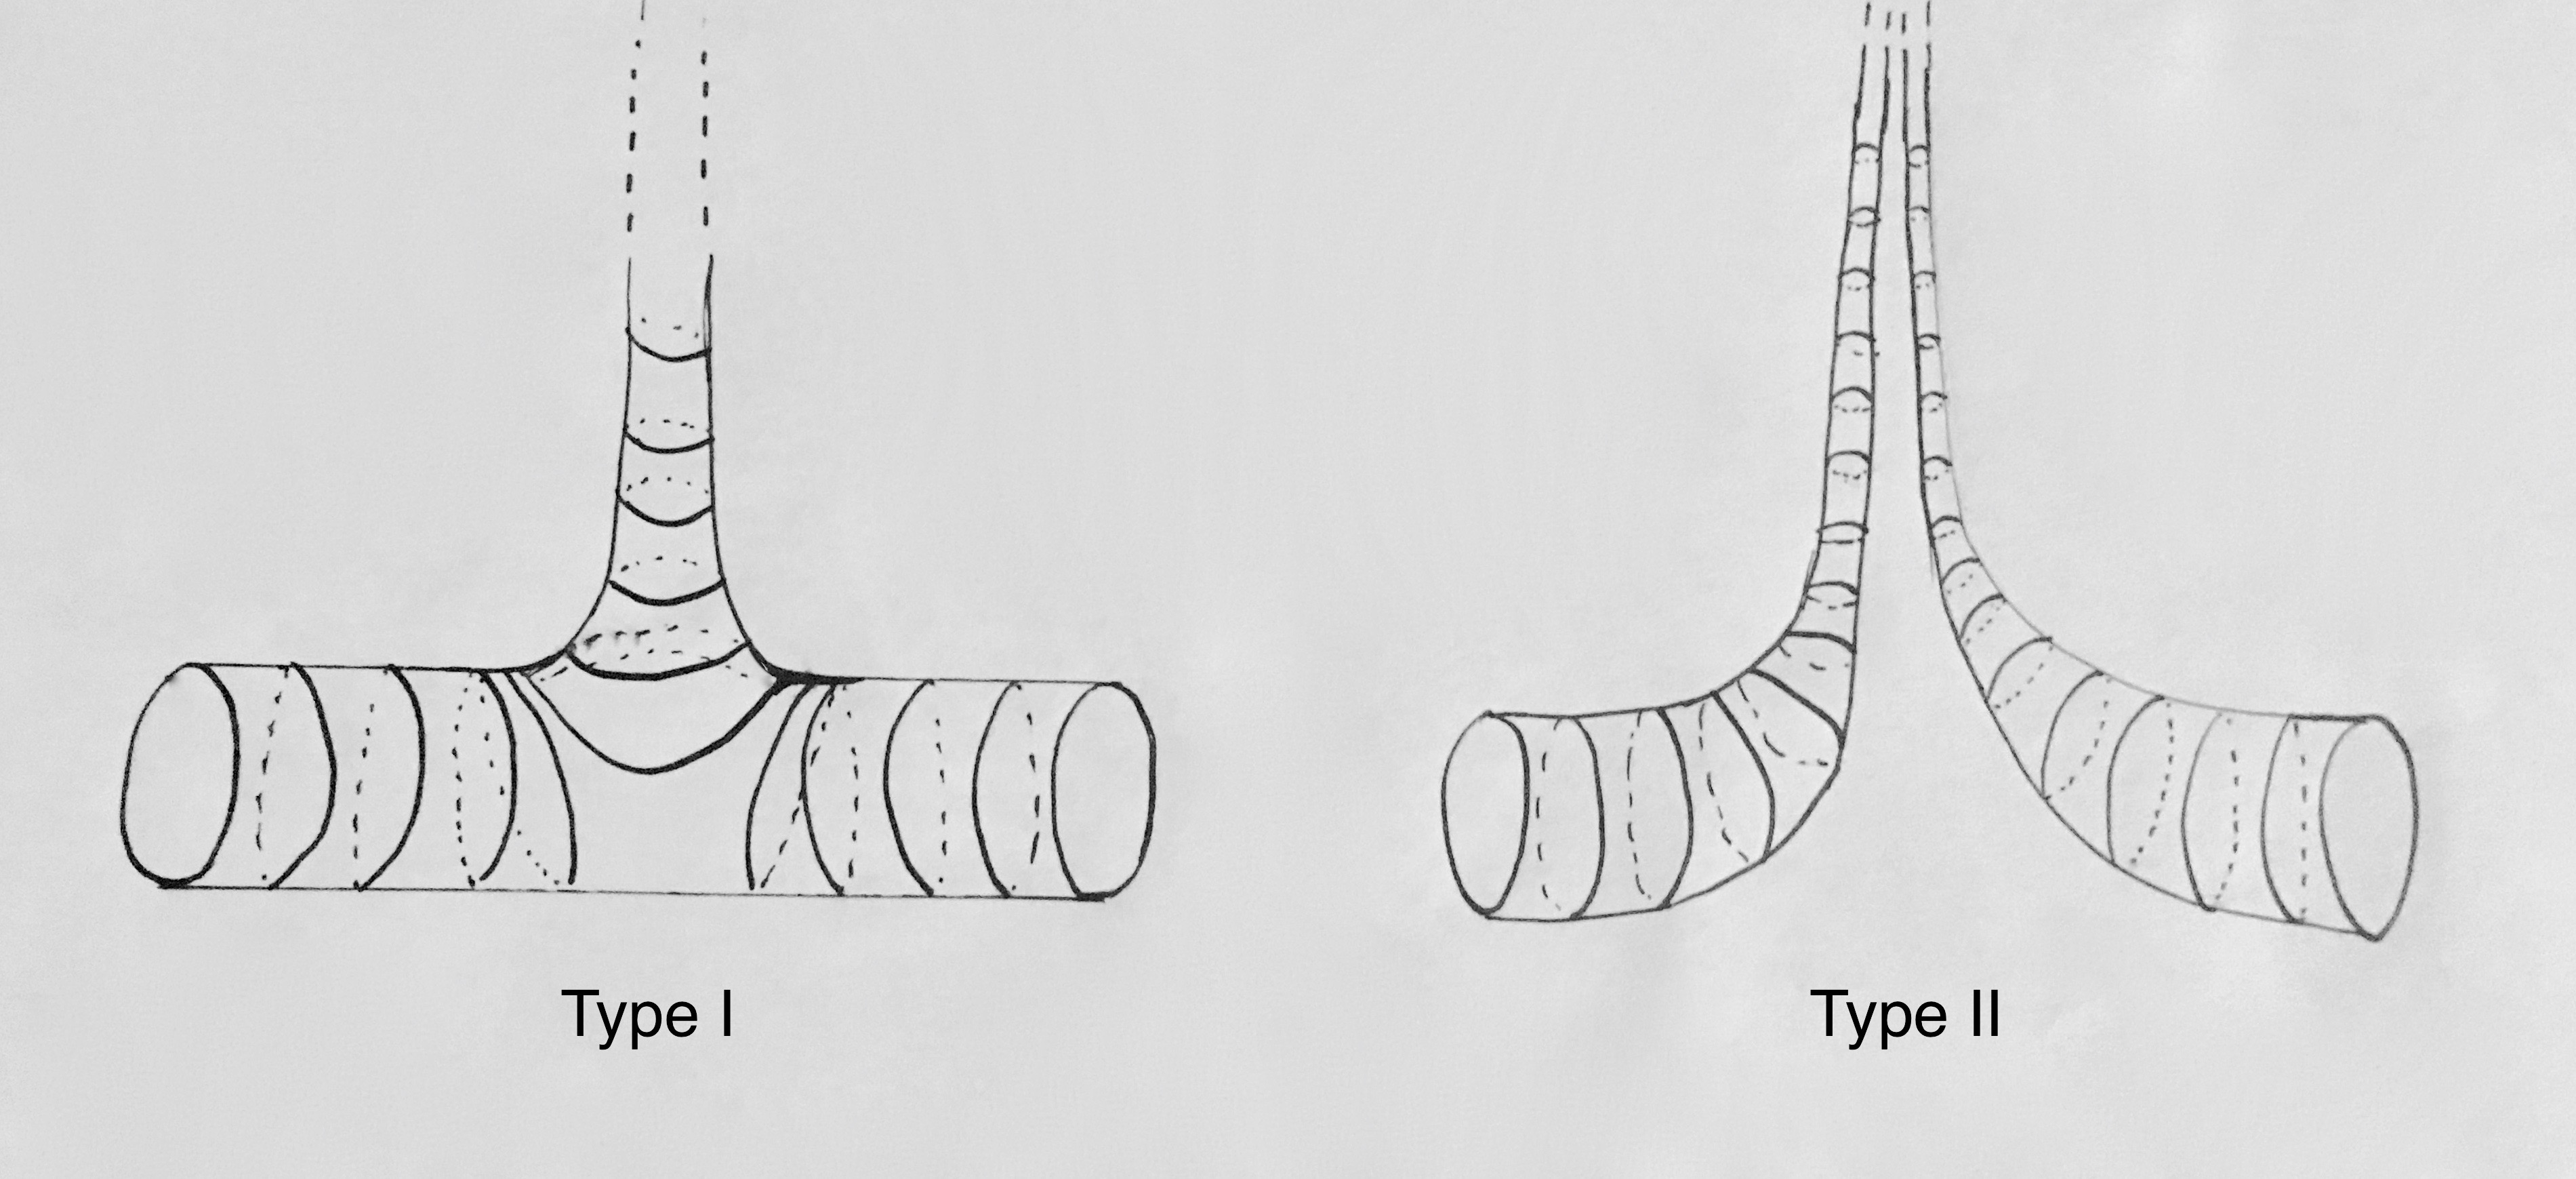
\includegraphics[scale=0.09]{SingularityType}
\caption{Two types of divergence}
\end{figure}

In the text below we introduce two conditions, one for ruling out each divergence. For the first type of divergence we introduce the condition of intermittent boundedness, or, i-boundedness. It involves bounds on the geometry of an associated metric on the Hamiltonian mapping torus which are required to hold on a sufficiently large subset of $M$. This condition is introduced first for the case where $H=0$ in \S \ref{Sec1} where we show that it provides diameter control. The condition of i-boundedness is framed so as to be contractible by allowing zig-zag homotopies. In \S \ref{Sec3} we discuss a trick which allows us to obtain the same diameter control for $H$ non-zero provided we restrict attention to fixed compact sets of the domain. When $H$ is non-zero, we are considering a geometry which is determined not just by $J$ but also by $H$. Most of \S\ref{Sec3} is devoted to studying the geometry of this metric.


To rule out the second type of divergence we introduce a number of variants of Palais-Smale type conditions. These properties are referred to collectively as loopwise dissipativity. These apply to the parametrized case if the $s$-dependence is compactly supported. This condition is likely not contractible. But this is not a problem since it only needs to be satisfied on the ends. In this it is similar to the non-degeneracy condition which is usually require in Floer theory. Note that unlike the property of i-boundedness, the property of loopwise dissipativity is not readily verifiable on non-exact submanifolds for Hamiltonians that do not have a small Lipschitz constant. In those cases it requires some understanding of the Hamiltonian flow.

Floer data satisfying these conditions are called \textbf{dissipative}.

We discuss three classes of examples of dissipative $(H,J)$.
\begin{enumerate}
\item $H$ is Lipschitz with respect to $g_J$ with sufficiently small Lipschitz constant outside of a compact set. More generally, mainly to allow a cofinal set, we  require the Lipschitz condition only on a sufficiently large subset of $M$. This class of examples is sufficient for all the theoretical constructions of this paper.
\item $M$ is exact and the action functional satisfies the Palais-Smale condition. See \S\ref{SubSec52}.
\item The Hamiltonian flow of $H$ is sufficiently close to being invariant with respect to a radial parameter. See \S\ref{SubsecNonex}.
\end{enumerate}
The following sections \S\ref{Sec1} through \S\ref{Sec5} are devoted to the construction of dissipative Floer data. They are organized as follows. In \S\ref{Sec1} we introduce the notion of i-boundedness, establish its  contractibility and derive various versions of diameter estimate it implies. In \S\ref{Sec3} we introduce the Floer equation and the Gromov metric. We introduce the notions of i-bounded and geometrically dissipative almost Floer data. Finally, we study the geometry of the Gromov metric for translation invariant Floer data. In \S\ref{Sec5} we study various aspects of the property of loopwise dissipativity and establish a diameter estimate as well as some effective criteria.
\section{I-bounded almost complex structures}\label{Sec1}
For a Riemannian metric $g$ on a manifold $M$ and a point $p\in M$ we denote by $\inj_g(p)$ the radius of injectivity and by $\Sec_g(p)$ the maximal sectional curvature at $p$. We drop $g$ from the notation when it is clear from the context.

\begin{df}\label{dfIntBounded}
Let $(M,g)$ be a complete Riemannian manifold. For $a>0$, the metric $g$ is said to be \textbf{$a$-bounded} at a point $p\in M$ if $\inj(p)\geq\frac1a$ and $|\Sec(x)|\leq a^2$ for all $x\in B_{1/a}(p)$.


We say that $g$ is \textbf{intermittently bounded}, abbreviated \textbf{i-bounded}, if there is an exhaustion $K_1\subset K_2\subset \dots$ of $M$ by precompact sets and a sequence $\{a_i\}_{i\geq 1}$ of positive numbers such that the following holds.
\begin{enumerate}
    \item $d( K_i,\partial K_{i+1})> \frac1{a_i}+\frac1{a_{i+1}}.$
    \item $g$ is $a_i$-bounded on $\partial K_i$.
    \item
        \begin{equation}\label{Eqtame}
            \sum_{i=1}^{\infty}\frac1{{a_i}^2}=\infty.
        \end{equation}
\end{enumerate}
The data $\{K_i,a_i\}_{i\geq 1}$ is called taming data for $(M,g)$.

For a symplectic manifold $(M,\omega)$, an $\omega$-compatible almost complex structure $J$ is called \textbf{i-bounded} if there exists an i-bounded Riemannian metric $g$ with taming data $\{K_i,a_i\}$ and constants $C_i$ such that
\begin{enumerate}
    \item
        \begin{equation}\label{Eqtame}
            \sum_{i=1}^{\infty}\frac1{{(C_ia_i)}^2}=\infty.
        \end{equation}
    \item
        $g_J$ is $C_i$-quasi-isometric to $g$ on $B\left(K_i,\frac1{a_i}\right)$. Namely,
        \[
            \frac1{C_i}\|X\|_g \leq \|X\|_{g_J}\leq C_i\|X\|_g
        \]
        on $B\left(K_i,\frac1{a_i}\right)$.
\end{enumerate}
The symplectic form $\omega$ is said to be \textbf{i-bounded} if it admits an i-bounded almost complex structure. For an i-bounded $(M,\omega)$ denote by $\mathcal{J}_{i.b.}(M,\omega)$ the space of i-bounded almost complex structures.

A $k$-parameter family $(g_t)_{t\in[0,1]^k}$ of i-bounded Riemannian metrics on $M$ is said to be \textbf{uniformly i-bounded}, or \textbf{u.i.b.}, if there is an $\epsilon>0$ such that for each $t_0\in [0,1]^k$ the taming data $\{K_i,a_i\}$ can be chosen fixed on the $\epsilon$ neighborhood of $t_0$.
 \begin{comment}
 and for each $i$, the restriction of $g$ to $B_{1/a}(\partial K_i)$ is quasi-isometric to a fixed metric on the same neighborhood.
\end{comment}
A family $\{J_t\}$ of almost complex structures is called \textbf{u.i.b.} if the corresponding family $\{g_{J_t}\}$ of Riemannian metrics is uniformly i-bounded.
\end{df}
\begin{ex}
If $J$ is geometrically bounded, meaning that $g_J$ is $a$-bounded everywhere for some $a$, it is i-bounded. In this case, we can take the taming data to be $\{K_i=B_{3i/a}(p),a_i=a\}$ for some arbitrary point $p\in M$.
\end{ex}
\begin{comment}

Before proceeding, we motivate the various parts of this definition. By the monotonicity inequality of \cite{Sikorav94}, stated below as Theorem~\ref{tmMonontonicity}, a $J$-holomorphic curve passing through an $a$-bounded point loses an amount of energy proportional to $\frac1{a^2}$. Thus, if $J$ is i-bounded then  for any $i\in \N$ and $E\in\R$ there is a number $N=N(i,E)$ such that a closed $J$ holomorphic curve intersecting $K_i$ and having energy at most $E$ is contained in $K_{i+N}.$
\end{comment}
\begin{rem}\label{rmGeoBCont}
The condition of i-boundedness is framed so that it simultaneously guarantees the conclusions of Theorems~\ref{tmWeakTameCont} and ~\ref{tmDiamEst} below. Namely, the condition is contractible, but still allows apriori control of the diameters of $J$-holomorphic curves. If we were to require boundedness everywhere, not just near $\partial K_i$, it appears unlikely to get a contractible condition as required in invariance proofs\footnote{As evidence for this consider that one can show using the result of \cite{Nab96} that the space of complete Riemannian metrics inducing a given volume form and having bounded geometry is disconnected. In fact, it has infinitely many connected components.}.
\end{rem}
 \begin{rem}
 Theorem \ref{tmWeakTameCont} below will remain true if we impose more stringent requirements on the numbers $a_i$, say, that they be bounded by a given constant. The reason we allow the numbers $a_i$ to diverge (subject to~\eqref{Eqtame}) is that in the context of Floer theory some times there naturally arise almost complex structures with associated metrics that do not have uniformly bounded sectional curvature. Example are the Sasaki metric on the cotangent bundle and the induced metric on the mapping torus of a quadratic Hamiltonian on the completion of a Liouville domain.
\end{rem}
\begin{comment}
The first main theorem we prove is
\begin{tm}\label{tmGdCont}
The set $\mathcal{J}_{i.b.}(\omega)$ is contractible.
\end{tm}

Theorem~\ref{tmGdCont} is given a more precise formulation below as Theorem~\ref{tmWeakTameCont} and is proven there.
\end{comment}
\begin{rem}
Note that  if $J$ is i-bounded and $J'$ is such that $\|J-J'\|_{g_J}$ is bounded, then $J'$ is i-bounded.
\end{rem}








\begin{tm}\label{tmWeakTameCont}
The space $\mathcal{J}_{i.b.}(M,\omega)$ is connected. Moreover, any two elements can be connected by a u.i.b. family. Similarly, any two uniformly  tame $k$-parameter families can be connected by a u.i.b. $k+1$-parameter family.
\end{tm}
\begin{rem}
The idea of the proof is very similar to the that of Proposition 11.22 in~\cite{CielEli}.
\end{rem}
\begin{proof}
Let $J_0,J_1\in\mathcal{J}_{i.b.}$. Given taming  data $\{K^i_n,a^i_n\}_{n\geq 1}$ for $J_i,i=0,1$, let $(c^i_n,d^i_n)_{n\geq 1}$ be sequences of positive integers constructed inductively such that the following holds.
\begin{enumerate}
\item\label{itDisja}
\[
\overline{K^0}_{d^0_n+c^0_n}\subset K^1_{d^1_n},\qquad \overline{K^1}_{d^1_n+c^1_n}\subset K^0_{d^0_{n+1}},\qquad\forall n.
\]
\item\label{itDisjb}
\[
\sum_{k=d^i_n+1}^{d^i_{n+c_n-1}}\left(\frac1{a^i_k}\right)^2\geq\frac1{n},\qquad i=0,1.
\]
\end{enumerate}
Write $V^i_n:=\overline{K^i}_{d^i_n+c^i_n}\setminus K^i_{d^i_n}$ for $i=0,1$. The sets $V^i_n$ are all disjoint by~\ref{itDisja}.  Let $\{J_s\})_{s\in[0,1]}$ be a smooth homotopy connecting $J_0$ and $J_1$ which is fixed and equal to $J_1$ on the subsets $V^0_n$ for all $s\in[0,2/3]$ and to $J_1$ on the subsets $V^1_n$ for all $s\in[1/3,1].$ Let
\[
A^i:=\cup_n[d^i_n+1,d^i_n+c^i_n-1]
\]
for $i=0,1$.  By~\ref{itDisja} and~\ref{itDisjb}, the data
\[
\left\{K^i_{n^i_k},a^i_{n^i_k}\right\}_{n_k\in A^i},\qquad i=0,1,
\]
constitute taming data for $J_s$ on the intervals $[0,2/3]$ and $[1/3,1]$ respectively. Moreover, for each $s\in[0,1]$ the metric $g_{J_s}$ is complete. Indeed, the  distance of  $\partial K^i_{n_k}$ from any fixed point goes to $\infty$ for $i=0$ and $s\in[0,2/3],$ and for $i=1$ and $s\in [1/3,1]$. We have thus connected $J_0$ and $J_1$ in a uniformly tame way.
\begin{figure}[h]
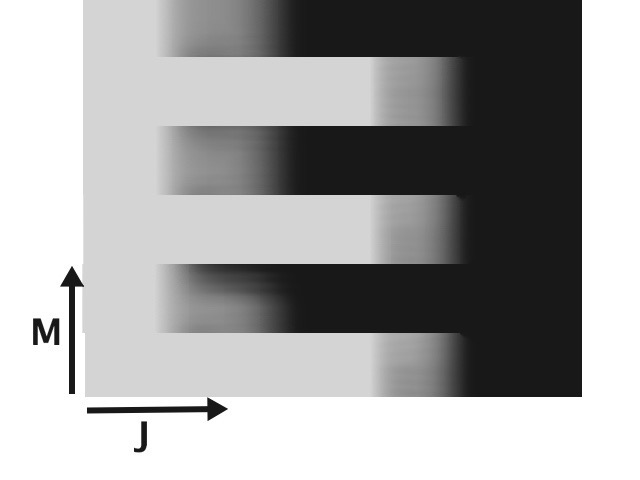
\includegraphics[scale=0.5]{Zig-Zag-Homotopy}
\caption{A Zig-Zag homotopy from $J_0$ (light) to $J_1$ (dark). }
\end{figure}
We now generalize to the $k$-parameter case. Let $\{J_{i,t}\}_{t\in[0,1]^k}$ for $i=0,1$ be two smooth $k$-parameter families.  Let $C$ be an open cover of the cube $[0,1]^k$ by open cubes of side length $\epsilon$ for $\epsilon$ so small that the taming data for both families can be chosen fixed on each such cube. For each $c\in C$ and $i\in \{0,1\}$ we construct precompact open subsets $\{V^{i,c}_n\}$ in such a way that
\begin{enumerate}
\item
$V^{i_1,c_1}_{n_1}$ is disjoint from $V^{i_2,c_2}_{n_2}$ whenever $(i_1,c_1,n_1)\neq (i_2,c_2,n_2)$
\item
There is taming data supported in $\cup_{n=1}^{\infty}V^{i,c}_n$ for $\{J_{i,t}\}_{t\in c}$ where we say that the taming data $\{K_i,a_i\}_{i\geq 1}$ is supported in an open set $V\subset M$ if $V$ contains all the balls $B_{1/a_i}(\partial K_i)$.
\end{enumerate}
Such sets can be constructed inductively along the same lines as in the $0$-parameter case. We can then take any smooth homotopy
\[
\{J_{s,t}\}_{(s,t)\in[0,1]\times[0,1]^k}
\]
which is fixed on all the subsets $\{V^{0,c}_n\}$ for $s\in[0,2/3]$ and on all the subsets $\{V^{1,c}_n\}$ for $s\in [1/3,1]$.
\end{proof}
For a $J$ holomorphic curve $u:S\to M$ denote by $E(u;S)$ the energy
\[
\int_Su^*\omega
\]
of $u$ on $S$. We drop $S$ from the notation when it is clear from the context.

The following theorem is taken from \cite{Sikorav94}.
\begin{tm}\label{tmMonontonicity}[\textbf{Monotonicity}]
Let $g_J$ be $a$-bounded\footnote{As the proof shows, we only need an estimate from above on the sectional curvature. The  stronger requirement is needed later in \S\ref{subsubinj}.} at $p\in M$. Let $\Sigma$ be a compact Riemann surface with boundary and let $u:\Sigma\to M$ be $J$-holomorphic such that $p$ is in the image of $u$ and such that
\[
u(\partial \Sigma)\cap B_{1/a}(p)=\emptyset.
\]
Then there is a universal constant $c$ such that
\[
E\left(u;u^{-1}(B_a(p))\right)\geq\frac c{a^2}.
\]
If $g_J$ is quasi-isometric to an $a$-bounded metric with quasi-isometry constant $A$, the same inequality holds but with $c$ replaced by $\frac{c}{A^2}$.
\end{tm}

\begin{proof}
This just a reformulation of the monotonicity inequality in \cite{Sikorav94}. See Proposition 4.3.1(ii) and the comment right after Definition 4.1.1 there. For completeness, we add a statement and proof of that comment in Lemma~\ref{lmIsopCurv} as we didn't find a proof of it in the literature.
\end{proof}

\begin{lm}\label{lmIsopCurv}
Let $g$ be Riemannian metric which is $a$-bounded at $p\in M$. Then any loop $\gamma:S^1\to B_{1/a}(p)$ bounds a disk of area less than $\frac12\ell^2(\gamma).$
\end{lm}
Our proof is taken from \cite{MS2}, the only addition being the precise dependence on the curvature.
\begin{proof}
Let $\tilde{\gamma}:S^1 \to T_pM$ be the unique path such that $\exp_p\tilde{\gamma}(\theta)=\gamma(\theta)$. Consider the disk $u(r,\theta)=\exp_pr\tilde{\gamma}(\theta)$. Since the geodesics emanating from $p$ minimize distance within $B_{1/a}(p)$, we have
\[
\|\partial_ru\|=\left\|\tilde{\gamma}(\theta)\right\|= d(\gamma(0),\gamma(\theta))\leq\frac12\ell(\gamma).
\]
We need to estimate the Jacobi field $J(r,\theta):=\partial_\theta u(r,\theta)$. For this we use the strong version of Rauch comparison theorem from \cite{Karcher}. Namely, we have that the function
\[
\frac{\|J(r,\theta)\|}{\sin ar}.
\]
is monotone nondecreasing on the interval $[0,\frac{\pi}{a}]$. So,
\[
\|J(r,\theta)\|\leq\|\gamma'(\theta)\|.
\]

Thus,
\[
\area(u)\leq\int_0^{2\pi}\int_0^1\|\gamma'(\theta)\| \frac12\ell(\gamma)drd\theta=\frac12\ell^2(\gamma).
\]
\end{proof}

The following theorem is fundamental for all that follows. It gives a priori control over the diameter of a $J$ holomorphic curve $u: \Sigma\to M$ with free boundary in terms of its energy.
\begin{tm}\label{tmDiamEst}
Let $J\in \mathcal{J}_{i.b.}$.
\begin{enumerate}
\item\label{tmDiamEstc1} For any compact set $K\subset M$ and $E\in\R_+$ there exists an $R>0$ such that for any connected compact Riemann surface $\Sigma$ with boundary and any $J$-holomorphic map
\[
u:(\Sigma,\partial\Sigma)\to (M,K)
\]
satisfying $E(u;\Sigma)\leq E,$ we have $u(\Sigma)\subset B_R(K)$.
\item\label{tmDiamEstc2}
  Let $\Sigma$ be a connected compact Riemann surface with boundary. For any compact set $K\subset M$, any compact subset $S$ of the interior of $\Sigma$ and any $E\in\R_+,$ there exists an $R$ such that for any $J$-holomorphic map
\[
u:\Sigma\to M
\]
satisfying $E(u;\Sigma)\leq E$ and $u(S)\cap K\neq\emptyset$ we have $u(S)\subset B_R(K)$.

 \end{enumerate}
In both cases, besides the dependence on $E$ and on $S$, $R$ depends only on taming data of $J$ inside $B_R(K)$. That is, given $J'$ which has the same taming data as $J$ on $B_R(K)$, the claim will hold with the same $R$ for $J'$-holomorphic curves with energy at most $E$.
\end{tm}

\begin{rem}
The reader should be careful to note that in case~\ref{tmDiamEstc2} where there is no control over the image of the boundary, to control the diameter of $u(S)$  we need control of the energy in the larger surface $\Sigma$.
\end{rem}
\begin{rem}
A remark is in order concerning the dependence of $R$ on the geometry in case~\ref{tmDiamEstc2}. In addition to the dependence on the taming data and on $E$, $R$ depends on the distance $d( S,\partial\Sigma)$ with respect to any conformal metric of a priori bounded curvature.
\end{rem}

\begin{proof}
Let $\{K_i,a_i\}$ be taming data for $J$. Let $N\in\Z$ be such that $K\subset K_N$. Let $i_0>0$ and $x_{i_0}\in\Sigma$ be such that $u(x_{i_0})\in\partial K_{i_0+N}$. If no such $i_0$ and $x_{i_0}$ exist we take $R=d(K,K_{N+1})$ and we are done. Otherwise, there is a sequence $x_i\in\Sigma$ such that $u(x_i)\in\partial K_{N+i}$ for $0<i\leq i_0$.
In case~\ref{tmDiamEstc1} we argue as follows. For each $1\leq i\leq i_0$, we have $b_{1/a_{N+i}}(u(x_i))\cap u(\partial \Sigma)=\emptyset$. Also,
\[
d(u(x_i),u(x_j))>\frac1{a_{N+i}}+\frac1{a_{N+j}},
\]
whenever $i\neq j$. By the monotonicity inequality we obtain
\[
E(u;\Sigma)\geq\sum_{i=1}^{i_0}E\left(u;u^{-1}(b_{1/a_{N+i}}(u(x_i))\right)\geq \sum_{i=1}^{i_0}\frac{C}{a^2_{i+N}}.
\]
By \eqref{Eqtame} this implies an a priori upper bound on $i_0$. Let $i_0$ be the largest possible such. The claim then holds with $R=d(K,K_{N+i_0+1})$.

In case~\ref{tmDiamEstc2} we argue as follows. Pick an area form $\omega_{\Sigma}$ on $\Sigma$ which together with $j_\Sigma$ determines a metric whose sectional curvature is bounded in absolute value by $1$. Let $A=\int_{\Sigma}\omega_{\Sigma}$ and let $\epsilon:=d(S,\partial\Sigma)$.  Let
\[
\tilde{u}=id\times u:\Sigma\to \Sigma\times M,
\]
and let $\tilde{J}$ be the product almost complex structure on $\Sigma\times M$. Then $\tilde{u}$ is $J$-holomorphic and $E(\tilde{u})= E(u)+A$. For any $x\in\Sigma$, any $p\in M$ and any $a\geq 1$ such that $(M,g_J)$ is $a$-bounded at $p$ we have that $(\Sigma\times M,g_{\tilde{J}})$ is $a$-bounded at $(x,p)$. Moreover, defining $x_i$ as before for points $x_i\in S$, the ball of radius $\min\left\{\frac1{a_{i+N}},\epsilon\right\}$ around $\tilde{u}(x_i)=(x_i,u(x_i))$ does not meet $\tilde{u}(\partial\Sigma)$. Thus, arguing as before, we have
\[
E(u;\Sigma)+A=E(\tilde{u};\Sigma)\geq\sum_{i=1}^{i_0}C\min\left\{\frac1{a^2_{i+N}},\epsilon^2\right\}.
\]
The claim follows as before.

\end{proof}
The final ingredient we shall need is the following elementary observation whose proof we leave for the reader.
\begin{tm}\label{tmPullbackTame}
The pullback of a u.i.b. family by a uniformly continuous map is u.i.b.
\end{tm}
Theorem~\ref{tmWeakTameCont} has consequences for symplectic invariants on open manifolds which we state as the following theorem.
\begin{tm}\label{TmSympInvGWSH}
The following invariants whose definition requires fixing geometrically bounded almost complex structure $J$ are independent of the choice of such $J$.
\begin{enumerate}
\item
The Gromov-Witten theory on geometrically bounded manifolds studied in \cite{Lu06}.
\item
Symplectic homology of relatively compact open sets studied in \cite{CielGinzKer}\footnote{See Remark 3.3 in \cite{CielGinzKer} where this question is raised.}.
\item
Rabinowitz Floer homology of tame stable Hamiltonian hypersurfaces in geometrically bounded manifolds \cite{cieliebak2010}\footnote{See the beginning of \S 4.5 in \cite{cieliebak2010}.}.
\end{enumerate}
\end{tm}
\begin{proof}
By Theorem~\ref{tmWeakTameCont} we can connect any two such almost complex structures $J_0$ and $J_1$ via a path $J_s$ of i-bounded almost complex structures. By Theorem~\ref{tmDiamEst} below the $J_s$-holomorphic curves of energy $\leq E$ with boundary in a given compact set $K$ are contained in a compact set $K'(E,K)$. Thus, standard cobordism or continuation arguments can be applied.
\end{proof}
\begin{rem}\label{rmGW}
The question of what kind of deformation of the symplectic structure preserves which of these invariants appears to be more subtle and is not studied here. In a forthcoming work, the question is taken up for particular type of deformation on Liouville domains.
\end{rem}
\begin{rem}
It is not known to the author whether the class of i-bounded symplectic manifolds is strictly larger than the class of geometrically bounded symplectic manifolds. It appears likely that it might be easier to characterize the class of i-bounded symplectic manifolds in terms of the topology of $\omega$. Call a symplectic manifold complete if for any disconnecting compact hypersurfaces $\Sigma$, a component of $M\setminus \Sigma$ which has finite volume is precompact in $M$. An interesting question is whether there are any obstructions to weak boundedness on complete symplectic manifolds?

It is also an interesting question whether finiteness of the total volume is an obstruction to weak boundedness, as it is to boundedness. In dimension $2$ the answer is clearly positive, but in higher dimension this is not clear to the author. If the answer is negative, it is possible that there are contact manifolds whose symplectization admit i-bounded almost complex structures allowing to define Floer theoretic invariants on them without recourse to symplectic field theory. This remark is due to A. Oancea.
\end{rem}
\section{Floer solutions and the Gromov metric}\label{Sec3}
\subsection{The Floer-Novikov covering and Floer's equation}\label{SecFloerGrom}
Let $(M,\omega)$ be a symplectic manifold. Denote by $\mathcal{L}M$ the free loop space $C^{\infty}(S^1,M)$.  Let $I_{\omega},I_c:\pi_1(\mathcal{L}M)\to\R$ be given by integrating $\omega$ and the Chern class respectively. Let the \textbf{Floer-Novikov covering} $\widetilde{\mathcal{L}M}$ be the Abelian covering space of $\mathcal{L}M$ for which $i_*\pi_1(\widetilde{\mathcal{L}M})=\ker I_\omega\cap \ker I_c$ where $i_*\pi_1(\widetilde{\mathcal{L}M})=\pi_1(\mathcal{L}M)$ is the natural inclusion. Explicitly, the space $\widetilde{\mathcal{L}M}$ is constructed as follows. For each component $\mathcal{L}M_a$ of $\mathcal{L}M$ choose a base loop $\gamma_a$. Then $\widetilde{\mathcal{L}M_a}$  consists of equivalence classes of pairs $(\gamma,A)$ such that $\gamma\in\mathcal{L}M_a$, $A$ is a homotopy class of paths in $\mathcal{L}M_a$ starting with $\gamma_a$ and ending at $\gamma$, and the equivalence relation is $(\gamma,A_1)\sim(\gamma,A_2)$ if and only if $\omega(A_1)=\omega(A_2)$ and $c_1(A_1)=c_1(A_2).$

For a smooth function $H:S^1\times M\to \R$ and for any $t\in S^1$ denote by $X_{H_t}$ the unique vector field satisfying $dH(t,\cdot)=\omega(X_{H_t},\cdot).$
Fixing base loops on the components of $\mathcal{L}M$, define a functional $\mathcal{A}_H:\widetilde{\mathcal{L}M}\to \R$ by
\[
\mathcal{A}_{H}([\gamma,A]):=-\omega(A)-\int_0^{2\pi}H(\gamma(t))dt.
\]

Denote by $\mathcal{P}(H)\subset\mathcal{L}M$ the set of $1$-periodic orbits of $X_H$. Denoting by
\[
\pi:\widetilde{\mathcal{L}M}\to\mathcal{L}M,
\]
the covering map, let
\[
\widetilde{\mathcal{P}(H)}=\pi^{-1}(\mathcal{P}(H)).
\]
This is the same as the critical point set of $\mathcal{A}_H$. Each $\tilde{\gamma}\in \widetilde{\mathcal{P}(H)}$ carries an index $i_{rs}(\tilde{\gamma})$ which is well defined up to a global shift for each homotopy class of loops. Namely, for each homotopy class $a$ fix  a trivialization of $\gamma_a^*TM$. Then if $\tilde{\gamma}=(\gamma,A)$ trivialize $\gamma^*TM$ along $A$ by extending the trivialization along $\gamma_a$ and take the Robin-Solomon index of $\gamma$ with respect to this trivialization.

Given an $S^1$ parameterized family of almost complex structures $J_t$ on $M$, the gradient of $\mathcal{A}_{H}(\gamma)$ at $\gamma$ is the vector field
\[
\nabla\mathcal{A}_{H}(\gamma)(t):=J_t(\dot{\gamma}(t)-X_{H_t}(\gamma(t)))
\]
along $\gamma$. Note that the gradient field is independent of the choice of base paths.  A gradient trajectory is a path in (a covering of) loop space whose tangent vector at each point is the negative gradient at that point. Explicitly a gradient trajectory is a map
\[
u:\R\times S^1\to M,
\]
satisfying Floer's equation
\begin{equation}\label{eqFloTranInv}
\partial_su+J_t(\partial_tu-X_{H_t}\circ u)=0.
\end{equation}
We refer to such solutions as \textbf{Floer trajectories}. A Floer trajectory is \textbf{nontrivial} if there is a point such that $\partial_tu\neq X_H$.

More generally, let $\Sigma$ be a finite type Riemann surface with cylindrical ends. This means that $\Sigma$ is obtained from a compact Riemann surface by a finite number of punctures and that near each puncture we fix a conformal coordinate system $\psi:(a,b)\times S^1\to\Sigma$ such that either $(a,b)=(-\infty,0)$ or $(a,b)=(0,\infty)$. In the first case we call the puncture negative and in the second, positive. Let $\mathfrak{H}\in\Omega^1(\Sigma,C^{\infty}(M))$ be a $1$-form with values in smooth Hamiltonians such that near each puncture there is an $H\in C^{\infty}(S^1\times M)$ for which $\mathfrak{H}=Hdt$ there. We denote by $X_\mathfrak{H}$ the corresponding $1$-form with values in Hamiltonian vector fields. Let $J\in C^{\infty}(\Sigma,\mathcal{J}(\omega))$ and suppose $J$ is $s$ independent on the cylindrical ends. The datum $(\mathfrak{H},J)$ is called a \textbf{domain dependent Floer datum}.


Let $u:\Sigma\to M$ be smooth. For a $1$-form $\gamma$ on $\Sigma$ with values in $u^*TM$ write
\[
\gamma^{0,1}:=\frac12\left(\gamma+J\circ\gamma\circ j_\Sigma\right).
\]
A \textbf{Floer solution} on $\Sigma$ is a map $u:\Sigma\to M$ satisfying Floer's equation
\begin{equation}
(du-X_\mathfrak{H}(u))^{0,1}=0.
\end{equation}
Note that Equation~\eqref{eqFloTranInv} is a special case. We refer to $J$ and $\mathfrak{H}$ as the Floer data of $u$. The \textbf{geometric energy} of $u$ on a subset $S\subset\Sigma$ is defined as
\[
E_{\mathfrak{H},J}(u;S):=\frac1{2}\int_S\|du-X_\mathfrak{H}\|_J^2dvol_\Sigma.
\]
We omit any one of $\mathfrak{H}$, $J$ or $S$ from the notation when they are clear from the context.  Floer's equation reduces to the nonlinear Cauchy Riemann equation when $\mathfrak{H}(v)=\gamma\otimes Const$ for $\gamma$ a $1$-form on $\Sigma$. In this case the two definitions of the energy coincide. Namely, we have the identity
\begin{equation}\label{eqEnId}
\frac1{2}\int_S\|du-X_\mathfrak{H}\|^2=\frac1{2}\int_S\|du\|^2=\int_Su^*\omega.
\end{equation}
\subsection{The Gromov metric}\label{SecGrom}
Let $u:\Sigma\to M$ be a Floer solution for the Floer data $F=(\mathfrak{H},J)$. Define $J_F$ by
\[
J_F(z,x):=\left(\begin{matrix} j_{\Sigma}(z) & 0  \\ X_\mathfrak{H}(z,x)\circ j_\Sigma(z)-J(z,x)\circ X_\mathfrak{H}(z,x) & J(x) \end{matrix}\right).
\]
Let
\[
\tilde{u}=(id,u):\Sigma\to\Sigma\times M.
\]
Then $\tilde{u}$ is $J_F$ holomorphic. This construction is known as Gromov's trick. See, e.g., \cite[Ch. 8.1]{MS2}.
\textit{Henceforth, given a Riemann surface $\Sigma$ with cylindrical ends, we shall assume that it comes equipped with an area form which is compatible with the complex structure and coincides with the standard one $ds\wedge dt$ on the ends.}
Note that $J_F$ is not generally tamed by the product symplectic structure $\omega_{\tilde{M}}=\omega_{\Sigma}\times\omega_M$. However, we have the following lemma.
\begin{lm}\label{lmAssocSymp}
 Suppose $\{\mathfrak{H},\mathfrak{H}\}=0$ .Namely,  for any $z\in\Sigma$ and any pair $v_1,v_2\in T_z\Sigma$ we have
 \begin{equation}\label{EqPoisson}
 \{\mathfrak{H}(v_1),\mathfrak{H}(v_2)\}=0
 \end{equation}
Assume that for each $(z,x)\in\Sigma\times M$ we have
\begin{equation}\label{EqMonHom}
d\mathfrak{H}(z,x)|_{T_z\Sigma}\geq 0.
\end{equation}
Then the $2$-form
\[
\omega_\mathfrak{H}:=\omega_\Sigma\times\omega_M+d\mathfrak{H},
\]
is a symplectic form which is compatible with $J_F$.
\end{lm}
\begin{proof}
We only show that $\omega_\mathfrak{H}$ is a symplectic form. Closedness is clear, so we only need to show non-degeneracy. In local coordinates on $\Sigma$ write
\[
\mathfrak{H}=Hdt+Gds.
\]
Then
\[
d\mathfrak{H}=dH\wedge dt+dG\wedge ds +(\partial_sH-\partial_tG)ds\wedge dt.
\]
Suppose there is a vector $v=(v_1,v_2)\in \Sigma\times M$ for which $\iota_v\omega_\mathfrak{H}$ is the $0$-form. Then
\[
-\iota_{v_2}\omega_M=dt(v_1)dH+ds(v_1)dG.
\]
So, $v_2=aX_H+bX_G$ for appropriate constants $a,b\in\R.$ Since $\{H,G\}=0$ it follows that $\iota_{v_2}(dH\wedge dt+dG\wedge ds)=0$. Thus,
\[
\iota_{v_1}(\omega_\Sigma+(\partial_sH-\partial_tG)ds\wedge dt)=0.
\]
Our assumption is that the coefficient of $ds\wedge dt$ in nonnegative. It follows that $v_1=0$ which in turn implies $v_2=0$.
\end{proof}
\begin{rem}
More generally, if we replace the estimate~\eqref{EqMonHom} by
\begin{equation}\label{EqMonHom1}
d\mathfrak{H}(z,x)|_{T_z\Sigma}\geq -ads\wedge dt,
\end{equation}
for some constant $a$, we have that the form
\[
\omega_{\mathfrak{H},a}:=\omega_\mathfrak{H}+ads\wedge dt,
\]
is symplectic.

The Poisson bracket condition \eqref{EqPoisson} may also be weakened to the requirement that for any point $z\in\sigma$ and vectors $v_1,v_2\in T_z\Sigma$ we have
\begin{equation}\label{eqWeakPoisson}
|\{\mathfrak{H}(v_1),\mathfrak{H}(v_2)\}(x)|<a\|v_1\|\|v_2\|,\quad\forall x\in M.
\end{equation}
In that case, the form $\omega_{\mathfrak{H},a}$ will again be a symplectic form.
\end{rem}


\begin{lm}\label{lmTopGeoEnEst}
Let $\Sigma$ be a Riemann surface with cylindrical ends and let $(\mathfrak{H},J)$ be a domain dependent Floer datum on $\Sigma$. For any $(\mathfrak{H},J)$-Floer solution $u:\Sigma\to M$ satisfying \eqref{EqMonHom}, we have
\[
E(u;\Sigma)\leq\int_{\Sigma}\tilde{u}^*\omega_\mathfrak{H}-\omega_\Sigma.
\]
The expression on the right is called the topological energy and denoted by $E^{top}(u)$.
\end{lm}

\begin{proof}
Write in local coordinates $\mathfrak{H}=Hdt+Gds$. Then using the Floer equation and denoting by $d'$ the exterior derivative in the $M$ direction,
\begin{align}
\|du-X_\mathfrak{H}\|^2ds\wedge dt&=\omega(\partial_tu-X_H,X_G-\partial_su)ds\wedge dt\notag\\
&=u^*\omega+(d'H(\partial_su)+d'G(\partial_tu))ds\wedge dt\notag\\
&=u^*\omega+d\mathfrak{H}-(\partial_sH\circ u-\partial_tG\circ u))ds\wedge dt\notag\\
&\leq u^*\omega+d\mathfrak{H}.\notag
\end{align}
\end{proof}
Henceforth, we shall denote by $g_{J_F}$ the Riemannian metric determined by $\omega_\mathfrak{H}$ and $J_F$ and refer to it as the \textbf{Gromov metric.} When $\mathfrak{H}=Hdt$ we will also use the notation $J_H$ and $g_{J_H}$.

\begin{ex}\label{ExTransInv}
Let $\mathfrak{H}=Hdt$, where $H:M\to\R$ is smooth. Then one finds by a straightforward computation that
\[
g_{J_H}=\pi_1^*g_j + \pi_2^*g_J+g_{mixed},
\]
where $\pi_i$ are the natural projections and
\[
g_{mixed}=-g_J(X_H,\cdot)dt+\|X_H\|^2dt^2.
\]
\end{ex}


\begin{df}\label{dfFloDataWbounded}
Let $\Sigma$ be a Riemann surface with cylindrical ends. A domain dependent Floer datum $(\mathfrak{H},J)$ on $\Sigma$ is called \textbf{i-bounded} if
\begin{enumerate}
\item $\mathfrak{H}$ satisfies inequalities~\eqref{EqPoisson} and~\eqref{EqMonHom} (or, more generally, inequalities~\eqref{eqWeakPoisson} and~\eqref{EqMonHom1}).
\item There exists a finite open cover $C$ of $\Sigma$ such that for each $U\in C$ we have $J_{\mathfrak{H}}|_{\overline{U}\times M}\in\mathcal{J}_{i.b.}(\omega_\mathfrak{H})$ (or, more generally, $J_{\mathfrak{H}}\in\mathcal{J}_{i.b.}(\omega_{\mathfrak{H},a})).$
 \end{enumerate}
\end{df}

 \begin{df}\label{dfFloDataWboundedFamily}
 Let $\mathcal{S}$ be a manifold with corners. A compact family $\Sigma_{\{s\in\mathcal{S}\}}$ of (broken) Riemann surfaces with cylindrical ends together with a smooth choice  domain dependent i-bounded Floer data $(\mathfrak{H}_s,J_s)$  is called \textbf{admissible} if the following holds. Denote by $\pi:\overline{S}\to S$ the tautological bundle. Then there is a finite cover of $\overline{\mathcal{S}}$ by connected opens consisting of elements of two types: $Thick_{\mathcal{S}}$ and $Thin_{\mathcal{S}}$.  The elements of $Thick_{\mathcal{S}}$ are subsets of $\overline{S}$ of the form $U=V\times W$ where $W\subset\mathcal{S}$  and $V$ is a bordered Riemann surface whose area is bounded on $W$. The fibers of $\pi$ restricted to elements of $Thin_{\mathcal{S}}$ are generically cylinders (of finite, half infinite or infinite length) which may degenerate to nodes at the corners.  Moreover, for the thin elements we require that the Floer data be translation invariant on the  fibers of $\pi$ and that the area forms to coincide with $ds\wedge dt$. We say that the family $\mathcal{S}$  is \textbf{uniformly i-bounded } if for any thick element $U=V\times W$ there exist taming  data on $V\times M $ which are constant on $W$ and for any thin element $U$ the there exist taming data on $[-1,1]\times S^1\times M$ which are constant on $\pi(U)$.

\end{df}






We wish to establish effective criteria for i-boundedness of $J_F$. To do this we need to a criterion for completeness of the metric $g_{J_F}$. Then we need to discuss how to compute the curvature of $g_{J_F}$ and control its radius of injectivity in terms of the Floer data $J$ and $\mathfrak{H}$. We do this in the case where $\mathfrak{H}=Hdt$ for a time independent Hamiltonian $H$  as in Example~\ref{ExTransInv}. Since intermittent boundedness is preserved under quasi-isometry, this should be quite sufficient for applications insofar as Floer trajectories are concerned. The consideration of more general Floer solutions will be reduced to that of Floer trajectories.
\subsection{Completeness}
\begin{df}
Let $J$ be an almost complex structure. We say that an exhaustion function $H:M\to\R$ is \textbf{$J$-proper} if $H$ factors as $H=f\circ h$ for some proper smooth function $h:M\to\R$ which is $1$-Lipschitz with respect to the metric $g_J$ on $M$.
\end{df}
\begin{lm}\label{lmStrPrpEst}
Let $(H,J)$ be $J$-proper with $H=f\circ h$ and $\|h\|\leq 1$. For any function $g:[a,b]\to \R$ and any $\gamma:[a,b]\to M$ we have
\[
|h(\gamma(b))-h(\gamma(a))|^2\leq (b-a)\int_a^b\|g(t)X_{H}-\gamma'(t)\|^2 dt.
\]
\end{lm}
\begin{proof}
We have
\begin{align}
|h(\gamma(b))-h(\gamma(a))|^2&=\left|\int_a^b\langle\nabla h,\gamma'(t)\rangle dt\right|^2\notag\\
&=\left|\int_a^b\langle\nabla h_t,\gamma'(t)-g(t)X_H\rangle dt\right|^2\notag\\
&\leq(b-a){\int_a^b\|g(t)X_{H}-\gamma'(t)\|^2 dt}\notag.
\end{align}
We used  Cauchy-Schwartz, $\|\nabla h\|\leq 1$, and the fact that $X_H\perp\nabla h$.
\end{proof}
\begin{lm}\label{tmGradFacComp}
Suppose $(H,J)$ is $J$-proper. Then $\tilde{M}$ carries a proper function which is Lipschitz with respect to $g_{J_H}$.
In particular, the metric $g_{J_H}$ is complete.
\end{lm}
\begin{proof}
Let $H=f\circ h$ where $h$ is proper and Lipschitz with respect to the product metric. We show that it is Lipschitz with respect to $g_{J_H}$. It suffices to show that for any path $\tilde{\gamma}:[a,b]\to\tilde{M}$ lifting a path $\gamma:[a,b]\to M$ we have
\[
|h(\tilde{\gamma}(b))-h(\tilde{\gamma}(a))|^2 \leq (b-a)\int\|\tilde{\gamma}'\|^2_{g_{J_H}}.
\]
For each $s$ we can $g_{H_J}$-orthogonally decompose
\[
\tilde{\gamma}'(s)=v(s)+g(s)(X_H+\partial_t),
\]
where $v(s)\in TM$. We have
\[
\|\tilde{\gamma}'(s)\|^2_{g_{H_J}}\geq\|v(s)\|^2=\|\gamma'(s)-g(s)X_H\|^2_{g_J}.
\]
The claim follows by Lemma~\ref{lmStrPrpEst}.

To see that $g_{J_H}$ is complete observe that  for any $x$ we have that the ball of radius $R$ around $x$ in $\tilde{M}$ is contained in the compact subset
\[
h^{-1}([h(x)-R,h(x)+R]).
\]

\end{proof}
We conclude with a criterion for $J$-properness. Call a function $f:\R\to[1,\infty)$ tame if the primitive of $\frac1{f}$ is unbounded from above.
\begin{lm}\label{lmCompCrit}
Suppose there is a tame function such that
\[
\|\nabla H\|_{g_J}\leq f(H).
\]
Then $H$ is $J$-proper.
\end{lm}
\begin{proof}
Let $g$ be a primitive of $\frac1{f}$. We have
\[
\|\nabla (g\circ H)\|=g'\circ H\|\nabla H\|=\frac1{f\circ H}\|\nabla H\|\leq 1.
\]
By assumption $h:=g\circ H$ is proper. Moreover, $g$ is monotone (primitive of a positive function). So $H=g^{-1}\circ h$.
\end{proof}

\subsection{Curvature}We introduce some notation and recall some basic formulae in Riemannian geometry. We refer to \cite{pe} for details. Let $(M,g)$ be a Riemannian manifold and let $r:M\to\R$ be a distance function. This means that $\|\nabla r\|=1$. Write $\partial_r:=\nabla r$ and denote by $S$ the tensor $\nabla\partial_r$. Denote by $U_r$ the level sets of $r$. Denote by $R$ the curvature tensor of $M$, by $R^t$ the tangential component of $R$ restricted to $TU_r$ and by $R^r$ the curvature tensor of $U_r$. Also, write $R_{\partial_r}=R(\cdot,\partial_r)\partial_r.$

The following formulae, together with the symmetries of the curvature tensor, show that the full curvature tensor on $M$ is determined by the curvature of the level sets of $r$, by the tensor $S$ and by its first derivative.
\begin{equation}\label{eqRiem1}
-R_{\partial_r}=S^2+\nabla_{\partial_r} S,
\end{equation}
\begin{equation}\label{eqRiem2}
R^t(X,Y)Z=R^r(X,Y)Z-S(X)\wedge S(Y)Z,
\end{equation}
\begin{equation}\label{eqRiem3}
R(X,Y)\partial_r=(\nabla_XS)(Y)-(\nabla_YS)(X).
\end{equation}
The vectors $X$, $Y$ and $Z$ in the above formulae are all tangent to $U_r$. In the sequel, given a vector $V\in TM$  we will use the notation $\theta_{g,V}$ for the dual to $V$ with respect to $g$ and will drop $g$ from the notation when there is no ambiguity. We utilize the following formula for the covariant derivative of a vector field $X$
\begin{equation}\label{eqCovDer}
2\theta_{g,\nabla X}=d\theta_{g,X}+\mathcal{L}_Xg.
\end{equation}
This formula presents the decomposition of $\theta_{g,\nabla X}$ into a symmetric and an anti-symmetric bilinear form. For a proof see \cite{pe}.

Let $\mathfrak{H}=Hdt$, where $H:M\to\R$ is smooth. Since $g_{J_F}$ is translation invariant with respect to $s$, we restrict attention to sub-manifolds of $\R\times S^1\times M$ with fixed values of $s$, or, in other words, to $S^1\times M$ with the metric $g_{J_F}$ as computed in Example~\ref{ExTransInv}. The function $t$ (which is locally single valued) is a distance function on $S^1\times M$ with respect to this metric. Moreover, we have that $\nabla t=X_H+\frac{\partial}{\partial t}$.

\begin{tm}\label{tmCurvXH}
 We have $\nabla\nabla t=\frac12(\nabla^{g_J} X_H+\nabla^{g_J} X_H^*)\circ\pi$ where the superscript denotes conjugation with respect to the metric $g_J$ and $\pi:T(S^1\times M)\to TM$ is the $g_{J_{\mathfrak{H}}}$ orthogonal projection.
\end{tm}
\begin{proof}
Write $N=\nabla t$. By equation~\eqref{eqCovDer} we have
\[
2\theta_{\nabla N}=d\theta_{ N}+\mathcal{L}_{ N}g_{J_F}.
\]
Since $\theta_ N=dt$, we have $d\theta_{ N}=0$. We claim that $\mathcal{L}_Ng_{J_F}=\pi^*\mathcal{L}_{X_H}g_J$. To see this denote by $\psi_t$ the time $t$ flow of $X_H$ and let
\[
\phi:(-\epsilon,\epsilon)\times M \subset S^1\times M\to S^1\times M,
\]
be the map $(t,p)\mapsto (t,\psi_{t}(p))$. Then $\phi_*|_{T(\{t_0\}\times M)}=\psi_{t_0,*}$ and $\phi_*\partial_t=\partial_t+X_H=N$. In particular, $\phi^*g_{J_F}|_{S^1\times M}=\pi^*\psi^*_tg_J+dt^2$. Thus,
\begin{align}
\phi^*\mathcal{L}_{ N}g_{J_F}&=\mathcal{L}_{\partial_t}\phi^*g_{J_F\emph{}}\notag\\
&=\partial_t(\pi^*\psi^*_tg_J+dt^2)\notag\\
&=\pi^*\psi_t^*\mathcal{L}_{X_H}g_J\notag\\
&=\phi^*\pi^*\mathcal{L}_{X_H}g_J.
\end{align}

By~\eqref{eqCovDer} we have
\[
\mathcal{L}_{X_H}g_J=[\theta_{\nabla X_H,g_J}],
\]
where $[\alpha(\cdot,\cdot)]$ denotes the symmetrization. Thus,
\[
S=\frac12(\nabla^{g_J} X_H+\nabla^{g_J} X_H^*)\circ\pi.
\]

\end{proof}
We say that a Hamiltonian $H:M\to\R$ is Killing (with respect to some compatible almost complex structure $J$) if the flow of $X_H$ preserves $g_J$.
\begin{cy}\label{cyKilling}
Suppose $H$ is killing, then $\nabla\nabla t\equiv 0$.
\end{cy}
\subsection{Injectivity radius}\label{subsubinj}
We turn to discussing the control of the radius of injectivity of $g_{J_H}$. In the following lemmas fix a point $x_0=(s_0,t_0,p_0)\in \R\times S^1\times M$.
\begin{lm}\label{lmVolEst1}
 For any $r<\frac12$ We have
\[
\vol_{g_{J_H}}(B_r(x_0))> \frac{r^2}{9}\vol_{g_J}(B_{r/3}(p_0)).
\]
\end{lm}
\begin{proof}
Denote by $\psi_t$ the Hamiltonian flow of $H$. Since $X_H+\partial_t$ is perpendicular with respect to $g_{J_H}$ to hypersurfaces of constant $t$, we have that $B_r(x_0)$ contains the cylinder
\[
C\quad=\bigcup_{t\in [t_0-r/3,t_0+r/3]} [s_0-r/3,s_0+r/3]\times\{t\}
\times\psi_t(B_{r/3}(p_0))\]
Since $\psi_t$ preserves volume we have
\[
\vol_{g_{J_H}}(C)=\frac{r^2}{9}\vol_{g_J}(B_{r/3}(p_0)).
\]
\end{proof}
\begin{lm}\label{lmCheeger}
Let $(M,g)$ be an $n$ dimensional Riemannian manifold. Let $a>0$ and let $p\in M$ such that
\[
\vol_g\left(B_{\frac1a}(p)\right)\geq v_0\left(\frac1{a}\right)^n
\]
and such that $|Sec_g(x)|\leq a^2$ on $B_{\frac1a}(p)$. Then there is a constant $f=f(v_0,n)$, independent of $a$, such that $inj_g(p)\geq f(v_0,n)$.
\end{lm}
\begin{proof}
Cheeger's Lemma asserts as much for $a=1$. The claim follows by scaling.
\end{proof}
\begin{lm}\label{lmVolEst2}
Suppose $(M,g)$ is $a$-bounded at $p$. Then there is a constant $C=C(n)>0$ such that
\[
\vol_g(B_{1/a}(p))\geq C\left(\frac1{a}\right)^n.
\]
\end{lm}
\begin{proof}
By scaling, the claim is equivalent to the claim that there is a constant $C(n)>0$ such that a geodesic ball of radius $1$ with sectional curvature bounded by $1$ has volume at least $C(n)$. By the Jacobi equation, sectional curvature controls the derivatives of the metric in geodesic coordinates.  In particular there is an a priori estimate from below on the determinant of the metric in these coordinates for a small enough ball around the origin. The claim follows.
\end{proof}
\begin{tm}\label{injEst}
There is a constant $i=i(n)$ such that if $g_J$ is $a$-bounded at $p_0\in M$ then $inj_{g_{J_H}}(x)\geq\frac{i(n)}{a}$.
\end{tm}
\begin{proof}
Combining Lemmas~\ref{lmVolEst1} and~\ref{lmVolEst2} we have that there is a constant such that
\[
\vol_{g_{J_H}}(B_{1/a}(x))\geq \frac{1}{3^{n+2}}C(n)\left(\frac1{a}\right)^{n+2}.
\]
The claim follows by Lemma~\ref{lmCheeger}.
\end{proof}
\subsection{Some criteria for boundedness}
\begin{lm}
Suppose $g_J$ is $a$-bounded at $p\in M$ and $H$ is a time independent Hamiltonian such that
\begin{equation}\label{eqCovEst}
\max\left\{\left\|\nabla X_H(p)\right\|^2,\left\|\nabla^2X_H\right\|,\left\|\nabla_{X_H}\left(\nabla X_H+\nabla X_H^T\right)\right\|\right\}<a^2.
\end{equation}
Then for a constant $c=c(n)$ independent of $a$, we have that $g_{J_H}$ is $ca$-bounded at $p$.
\end{lm}
\begin{proof}
We need to estimate the sectional curvature and radius of injectivity of $g_{J_H}$. Up to multiplication by a constant dependent on $n$, estimating sectional curvature is the same as estimating the coefficients of the curvature tensor in an orthonormal basis. Since $J$ is $a$-bounded, it remains to estimate only coefficients involving the direction $\partial_t+X_H$ at least once. In light of formulae~\eqref{eqRiem1}-\eqref{eqRiem3} we need to estimate $\nabla S$ and $S^2$ where $S=\nabla t$. Theorem~\ref{tmCurvXH} provides us with an estimate on $S^2$ and the tangential restriction of $\nabla S$ in terms of $\nabla X_H$ and $\nabla^2 X_H$. It remains to estimate the right hand side of \eqref{eqRiem1}. For this it is preferable to use the formula
\[
-R_{N}=\mathcal{L}_{ N}S-S^2.
\]
See \cite{pe}. Each summand vanishes on $N$. So it remains to estimate $\mathcal{L}_{ N}S$ applied to a tangential vector. Let $V$ be a tangential vector field which commutes with $N.$ Then
\begin{align}
\mathcal{L}_{X_H+\partial_t}(SV)&=\mathcal{L}_{X_H}(SV)\notag\\
&=\nabla^{g_J}_{X_H}({S}V)-\nabla^{g_J}_{SV}(X_H)\notag\\
&=(\nabla^{g_J}_{X_H}{S})V+S(\nabla^{g_J}_V{X_H})-\nabla^{g_J}_{SV}(X_H)\notag.
\end{align}
This shows that estimate~\eqref{eqCovEst} implies $Sec_{g_{J_H}}(p)\leq c^2a^2$ for an appropriate $c=c(n)$. Theorem~\ref{injEst} provides us with the estimate on $inj_{g_{J_H}}$ in terms of $inj_{g_J}(p)$. The claim follows.
\end{proof}

The following Lemma whose proof is left for the reader is an alternative to invoking Lemma~\ref{eqCovEst} in some instances.
\begin{lm}\label{lmQuasHam}
Let $(H_1,J)$ be a Floer datum and let $H_2$ be a time dependent Hamiltonian such that $X_{H_2}\leq C$ for some constant $C$. Then $g_{H_1+H_2}$ is $C^2$-quasi-isometric to $g_{H_1}$. In particular, when $J$ is i-bounded and $H$ is such that $\|X_H\|$ is bounded we have that $J_{H}$ is i-bounded.
\end{lm}


\begin{ex}\label{ExLiouvTame}
Let $(\Sigma,\alpha)$ be a contact manifold and let
\[
(M=\R_+\times\Sigma,\omega=e^r(d\alpha+dr\wedge\alpha ))
\]
be the convex end of its symplectization. Denote the Reeb vector field on $\Sigma$ by $R$. Fix an $\omega$-compatible translation invariant almost complex structure $J$ satisfying $JR=\partial r$. Then
\begin{equation}\label{eqMetConvSymp}
g_J=e^r(dr^2+g_\Sigma),
\end{equation}
for some metric $g_\Sigma$ on $\Sigma$. Since the metric $g_J$ scales up, the radius of injectivity of $g_J$ is bounded away from $0$, and in fact goes to $\infty$ with $r$. Let now $H$ be a smooth time independent Hamiltonian. Pick local coordinates on $\Sigma$ and use the function $r$ as the coordinate on the $\R_+$ factor. Then  the left hand side of~\eqref{eqCovEst} is controlled by the squares of the partial derivatives of $H$ up to order $3$ in these coordinates. Indeed, applying the Koszul formula to the metric \eqref{eqMetConvSymp}, we have
\[
\langle \nabla_{\partial_i}\partial j,\partial_k\rangle\sim e^r.
\]
Since $\|\partial_i\|^2\sim e^r$, for some constant $C$ we have $\|\nabla \partial_i\|\leq C$. Similarly,
\[
\|\nabla^2_{ij}\partial_k\|^2\sim e^r,
\]
allowing us to deduce that
\[
\|\nabla^2\partial_k\|\sim e^{-r/2}.
\]
Thus, writing
\[
X_H=\sum f_i\partial_i,
\]
we find after writing everything out that the left hand side of~\eqref{eqCovEst} is controlled by the square of the derivatives up to order $2$ of the $f_i$.

\end{ex}

\begin{ex}\label{wxAdmWT}
Continuing with the previous example, let $h:\R\to\R$ satisfy that there exists a monotone sequence $t_i$ and a divergent series $\sum a_i$ such that the following hold.

\begin{enumerate}
\item
\[
\sqrt{t_{i+1}}-\sqrt{t_i}\geq \frac{1}{a_i}+\frac{1}{a_{i+1}}.
\]
\item
For any $t\in \left(\left(\sqrt{t_{i}}-\frac1{a_i}\right)^2,\left(\sqrt{t_i}+\frac1{a_i}\right)^2\right)$ we have
\[
\left(|h'(t)|+|h''(t)|+|h^{(3)}(t)|\right)^2\leq a_{i}^2 .
\]
\end{enumerate}
Then any $(H,J)$  on the symplectization where $H$ which is of the form $H=h(e^r)$ outside a compact set and $J$ is of contact type is geometrically dissipative. To see this, note that the function $e^r$ is roughly the square of the distance to $\Sigma$.

Suppose now the Reeb flow is Killing. Then we can relax the requirements on the first derivative of $h$. Namely we can allow the first derivative to be a constant of any size on the appropriate intervals.
\end{ex}
\begin{ex}
Consider the case of the cotangent bundle $T^*M$ of a compact manifold $M$, let $g$ be a Riemannian metric on $M$ and let $J$ be the Sasaki almost complex structure on $T^*M$. It is defined as follows: the Levy-Civita connection on $T^*M$ induces a splitting $TT^*M=V\oplus H$ into horizontal and vertical vectors. Moreover, we take  $J:V\simeq H$ to be the natural isomorphism identifying an element of $V$ with an element of $T^*M$, then via $\omega$ with an element of $TM$ and finally with an element of $H$ via horizontal lifting. Identifying $TM=T^*M$, in standard local Darboux coordinates $\{q_i,p_i=dq_i\}$, where $q_i$ are geodesic coordinates centered at a point $q$, $J$ is given in the fiber over $q$ by
\[
J\frac{\partial}{\partial p_i}=\frac{\partial}{\partial q_i}.
\]
Then it is easy to show that the metric $g_J$ is $\|p\|$-bounded at the point $(p,q)$. In particular, $J$ is i-bounded (but not bounded). Consider a Hamiltonian of the form  $H=\sqrt{a|p|^2+V\circ\pi}$, where $\pi:T^*M\to M$ is the standard projection and $V:M\to\R$ is smooth, $J_H$ is i-bounded. Indeed, denoting by $M$ the maximum of $\sqrt{|V|}$ over $M$ we have in local coordinates as above
\[
\|X_H\|=aM\frac1{2\|p\|}\left\|\sum_ip_i\frac{\partial}{\partial q_i}\right\|\leq aM.
\]
So, the claim follows from Lemma~\ref{lmQuasHam}. Note that mechanical Hamiltonians of the form $|p|^2+V\circ\pi$ are not i-bounded with respect to the Sasaki metric.
\begin{comment}
However, the isoperimetric inequality can be shown to hold for them with constants uniform over $T^*M$. Thus we would still have that $J_H$ is geometrically dissipative. We do not make use of this claim, so we do not prove it.
\end{comment}
\end{ex}

\section{Loopwise dissipativity}\label{Sec5}
\subsection{Diameter control of Floer trajectories}
Suppose $(H,J)$ is i-bounded, let $u$ be a Floer trajectory, and let $\tilde{u}$ be its graph. Suppose that for some precompact $U\subset \R\times S^1$, we have control over $u(\partial U)$. Theorem~\ref{tmDiamEst} above then provides with control over $u(U)$ in terms of
\[
E(\tilde{u};U)=E(u;U)+\area(U).
\]
This indicates that the only source of non-compactness in the moduli space of finite energy Floer trajectories comes from the potential existence of finite energy solutions with one end converging to infinity. This motivates the following definition.

Fix a point $p\in M$ and define a function $g_{H,J}(r_1,r_2)$ by $g_{H,J}(r_1,r_2)\leq E$ if there is a Floer trajectory of energy $E$ defined on a finite cylinder with one end in $B_{r_1}(p)$ and the other end in $M\setminus B_{r_2}(p)$.

\begin{df}
We say that $(H,J)$ is \textbf{loopwise dissipative on-shell (LDOS)} if for any $r_1$ we have that $g_{H,J}(r_1,r)$ is unbounded as $r\to\infty$. For any function $g:\R\times\R\to\R$ such that $g_{H,J}\leq g$, we say that $(H,J)$ is $g$-LDOS. We say that $(H,J)$ is \textbf{strongly LDOS} if there is a uniform (with respect to $g_J$) open neighborhood of $(H,J)$ in $C^1\times C^0$ which is LDOS.
\end{df}
Note that the choice of the point $p$ in the definition of $g$ is of no consequence.
\begin{df}
Denote by $\mathcal{F}_d^{(0)}(M)$ the set of i-bounded Floer data $(H,J)$ which are strongly LDOS. Elements of $\mathcal{F}_d^{(0)}(M)$ are referred to as \textbf{dissipative Floer data}.
\end{df}
Our next Theorem shows that dissipativity is all we need for diameter control. We have already seen how to verify the $i$-boundedness condition. In the ensuing sections we consider a number of quantitative (``off-shell") refinements of the LDOS condition. These refinements are used to show both that on a geometrically bounded manifold there is always a sufficient supply Floer data satisfying the LDOS condition and that this property can be verified directly in numerous settings.

In the following theorem recall Definitions \ref{dfFloDataWbounded} and \ref{dfFloDataWboundedFamily} of an i-bounded Floer datum and family of Floer data.
\begin{tm}\label{tmFloSolDiamEst}
Let $(\mathcal{S},F_{s\in S}=(\mathfrak{H}_{s},J_{s}))$  be a uniformly i-bounded family of (broken) genus $0$  Riemann surfaces with $i$ cylindrical ends. Let $(H_i,J_i)\in\mathcal{F}_d^{(0)}$ be Floer data such that on the $i$th end, $F_s$  coincides with $(H_i,J_i)$ for all $s\in\mathcal{S}$ . Then for any compact $K\subset M$ and any real number $E$, there is an $R=R(E,K)$  such that for any $s\in\mathcal{S}$ and any $F_s$-Floer solution $(\Sigma,u)$  with $E(u)\leq E$ and intersecting $\partial K$ is contained in $B_R(K)$. Moreover, if $K$ is a level set of $H$ with no degenerate periodic orbits in a neighborhood of $\partial K$, we can take $R(E,K)\to 0$ as $E\to 0$.
\end{tm}
\begin{proof}
By definition, we can decompose $\Sigma$  into a thick part consisting of components $A_i$ with a-priori bounded area and ends $B_i$ where the Floer data are translation invariant. The number of components is bounded a priori in terms of $\mathcal{S}$. For each $A_i$, the graph $\tilde{u}=id\times u :A_i\to A_i\times M$ is $J_F\emph{}$ holomorphic and has energy bounded by $E+Area(A_i)$. If $u|_{A_i}$ intersects some compact set $K$ then, since $\tilde{u}$ extends to a neighborhood of $A_i$, part \ref{tmDiamEstc2} of Theorem~\ref{tmDiamEst} applied to the graph $\tilde{u}$ implies that $u(A_i)$ is contained in a ball $B_R(K)$  for some $R$ depending only on the taming data. It follows that each of the ends $I_i$ has a boundary component contained in $B_R(K)$.  Loopwise Floer dissipativity on the ends $B_i$ implies there is an $R_1$ such that, writing $B_i=I\times S^1$ for some interval $I$, we have that $u(\{s\}\times S^1)$ intersects $B_{R_1}(K)$ for each $s\in I$. Restricting $u$ to $(s-1,s+1)\times S^1$ and invoking Theorem~\ref{tmDiamEst} again, we obtain the an $R_2$ such that for any $s\in I$, we have $u((s-1,s+1)\times S^1)\subset B_{R_2}(B_{R_1}(K))$.  In particular, the same holds for $u(B_i)$. Since the number of components is bounded a-priori, we obtain an $R$ as required.

For the last statement we rely on the following property of Floer trajectories which is stated in \cite{Salamon1999}. There are constants $c$ and $\hbar$ such that
\[
\int_{B_{r}(s,t)}\|\partial_su\|^2<\hbar\quad\Rightarrow\quad\|\partial_su\|^2(s,t)<\frac8{\pi r^2}\int_{B_{r}(s,t)}\|\partial_su\|^2+cr^2.
\]
Once we know that a solution is contained in an a-priori compact set, we can take all the constants to be fixed by that compact set. By taking $r=E(u)^{1/4}$ we deduce that for an appropriate constant
\[
\|\partial_tu-X_H\|^2=\|\partial_su\|^2<CE(u)^{1/2},
\]
once $E(u)$ is small enough. It follows that making $E(u)$ arbitrarily small, $u$ will be contained in an arbitrarily small neighborhood of some periodic orbit.
\end{proof}



We conclude this subsection with a counterexample showing that geometric boundedness alone does not guarantee loopwise dissipativity.
\begin{ex}\label{ExDegAtInfty}
Consider $(M,\omega)=(\R\times S^1,ds\wedge dt)$. Let
\[
H(s,t)=s-\ln (s+1),
\]
and let $J$ be multiplication by $i$. Then $(H,J)$ is readily seen to be i-bounded but it is not LDOS. Indeed, the map $u:\R_+\times S^1\to M$ defined by $u(s,t)=(\ln (s+1),t)$ is an $(H,J)$-partial Floer trajectory of finite energy and infinite diameter.
\end{ex}


\subsection{Loopwise dissipativity}
A path $\gamma:[a,b]\to\mathcal{L}M$ is \textbf{$\epsilon$-gradient} for a Floer datum $(H,J)$ if it satisfies
\[
\|\nabla\mathcal{A}_H(\gamma_s)-\partial_s\gamma\|<\epsilon,\quad \& \quad \max_{s\leq s'\in[a,b]}\{\mathcal{A}_H(\gamma_s)-\mathcal{A}_H(\gamma_{s'})\}<\epsilon.
\]
Define the energy of a path $\gamma:[a,b]\to\mathcal{L}M$ with respect to $H$ by
\[
E_H(\gamma)=\max\left\{\int_a^b\|\partial_s\gamma\|^2,\mathcal{A}_{H}(\gamma_a)-\mathcal{A}_H(\gamma_b)\right\}.
\]

We say that $(H,J)$ is \textbf{loopwise dissipative (LD)} if there is an $\epsilon>0$ which satisfies the following. For any compact set $K$ and any constant $E$ there is an $R=R(K,E)$ such that any $\epsilon$-gradient $\gamma:[a,b]\to\mathcal{L}M$ with $E(\gamma)<E$ and $\gamma_a\subset K$ satisfies $\gamma_b\cap B_R(K)\neq\emptyset$.

Informally, this means that it takes an infinite amount of energy to move a loop to infinity along a path which is not far from being gradient like.

\begin{lm}\label{lmWeakDisOp}
Suppose $(H,J)$ is LD. Then any $(H',J')$ sufficiently $C^1\times C^0$ close to $(H,J)$ with respect to the metric $g_J$ is LD.
\end{lm}
\begin{proof}
If $(H',J')$ is sufficiently $C^1\times C^0$ close to $(X_H,J)$ then for sufficiently small $\epsilon'$, an $\epsilon'$-gradient for $(H',J')$ is $\epsilon$-sub gradient for $(H,J)$. Moreover, the energies $H_H,E_{H'}$ and the metrics $g_J,g_{J'}$ are comparable.
\end{proof}


\begin{lm}\label{lmModBd}
Let $u:[a,b]\times S^1\to M$ be a differentiable map. Then we have
\[
(b-a)\geq\frac{\int_{t\in S^1}d^2(u(a,t),u(b,t))}{\int_{[a,b]\times S^1}\|\partial_su\|^2}.
\]
\end{lm}
\begin{proof}
By the Cauchy Schwartz inequality we have
\begin{align}
(b-a)\int_{[a,b]\times S^1}\|\partial_su\|^2&\geq \int_{t\in S^1}\ell^2(u(t\times [a,b]))dt\notag\\
&\geq \int_{t\in S^1}d^2(u(a,t),u(b,t))\notag.
\end{align}
\end{proof}

\begin{lm}\label{lmLoopDisQuant}
Suppose $(H,J)$ is $J$-proper. Then $(H,J)$ is LD if and only if the following holds. There is a constant $\delta>0$ and an exhaustion $\{K_i\}$ such that any $\epsilon$-gradient $u$ with negative end in $K_i$ and positive end in $M\setminus K_{i+1}$ satisfies
\[
E(u)>\delta.
\]
\end{lm}
\begin{proof}
One direction is obvious from the definition. In the other direction, suppose there is an $\epsilon>0 $ and an exhaustion as in the statement of the Lemma. We prove $(H,J)$ is loopwise dissipative by induction on the smallest integer $n$ bounding $E(u)/\delta$. When $n=1$, this just the assumption. Suppose we have proven the statement for all $\epsilon$-gradients satisfying $E(u)\leq n\delta$. Let $u$ be an $\epsilon$-gradient with negative end in $K_i$ and $E(u)\leq (n+1)\delta$. Let
\[
s_1=\inf \{s\in[a,b]:u_s\subset M\setminus K_{i+1}\}
\]
If this set is empty there is nothing to prove. Otherwise, let
\[
s_2=\inf\{s\in[s_1,b]:\|\partial_su\|<1\}\cup\{b\}.
\]
Finally, take
\[
s_0=\sup\{s\in[a,s_1]:\|\partial_su\|<1\}\cup\{a\}.
\]
We have $s_2-s_0<E$. So, by Lemma~\ref{lmModBd}, there is a $t\in S^1$ such that $d(u_{s_0}(t),u_{s_2}(t))<E$. By the estimate $\|\partial_{s}u_{s_i}\|<1$  we get $\|\nabla\mathcal{A}_H\|<1+\epsilon$ for $i=0,2$. Combining this, Lemma~\ref{lmStrPrpEst}, and the fact that $u_{s_0}$ meets $K_i$, we obtain an $i_0$ depending only on $E$ and $i$ such that $u_{s_2}\subset K_{i+i_0}$. We have $E(u|_{[s_2,b]})\leq n\delta$, so there is an $i_1$ depending on $i_0$ and $n$ such that $u_b$ meets $K_{i+i_0+i_1}$. The claim now follows.
\end{proof}

\begin{tm}\label{tmBoundGradDis}
Let $J$ be geometrically bounded. Then there is a $\delta>0$ such that any proper Hamiltonian with $\|X_H\|<\delta$ is LD. Moreover, it is dissipative.
\end{tm}
\begin{proof}
Let $u:[a,b]\times S^1\to M$ be an $\epsilon$-gradient such that
\[
\max_tH\circ u(a,t)<x_1<x_2<\min H\circ u(b,t).
\]
 Then
\begin{equation}\label{eqEnGradFlow}
E(u)\geq (x_2-x_1)-\int u^*\omega.
\end{equation}
We will show that if we take $\delta$ and $\epsilon$ small enough, there are constants $\delta_1,\delta_2$ such that $\left|\int u^*\omega\right|>\delta_1\Rightarrow E(u)>\delta_2$. It will then follow from~\eqref{eqEnGradFlow} that if $x_2-x_1>2\delta_1$ then $E(u)>\min\{\delta_1,\delta_2\}$ proving the claim by Lemma~\ref{lmLoopDisQuant}.

We show the existence of constants $\delta$, $\delta_1$ and $\delta_2$ as above. We take $\delta$ so small that any loop of length $2\delta$ has diameter less than the radius of convexity of $M$ with respect to $g_J$. The isoperimetric inequality guarantees there is a constant $c$ such that any loop of length $<2\delta$ is fillable by a disk $v:D\to M$ such that
\[
\int_Dv^*\omega\leq Area(v)<c\delta^2.
\]
We take $\epsilon=\delta$, $\delta_0=c\delta^2$ and $\delta_1=2\delta_0$. Given $u$ as above, let
\[
I=\{s\in[a,b]|\ell( u(s,\cdot))>2\delta\}.
\]
For any component $(c,d)$ of $I$ we have the estimate
\[
\left|\int_{(c,d)\times S^1}u^*\omega\right|\leq Area(u)\leq 3 E(u;{(c,d)\times S^1}).
\]
The first of these is Wirtinger's inequality. For the second, note that
\[
Area(u)\leq\int_{(c,d)\times S^1}\|\partial_su\|\|\partial_tu\|\leq \frac12\int_{(c,d)\times S^1}(\|\partial_su\|^2+\|\partial_tu\|^2),
\]
But,
\begin{align}
4\delta^2\leq\int_{S^1}\|\partial_tu\|^2&\leq \int_{S^1}\|\partial_tu-X_H\|^2+\int_{S^1}\|X_H\|^2\notag\\
&\leq \int_{S^1}\|\partial_su\|^2+\epsilon^2 +\delta^2\notag\\
&=\int_{S^1}\|\partial_su\|^2+2\delta^2\notag\\
&\leq \|\partial_su\|^2+\frac12\int_{S^1}\|\partial_tu\|^2\notag.
\end{align}
So,
\[
\|\partial_tu\|^2\leq2\|\partial_su\|^2
\]
which implies the desired inequality.

Suppose now that $|\int_{[a,b]\times S^1}u^*\omega|\geq 4\delta_1$. Then $I\neq\emptyset$. Otherwise, we could fill the boundary of $u$ by disks contained in a contractible ball of radius $\leq 2\delta$ and obtain a contractible sphere which would imply the contradiction $|\int_{[a,b]\times S^1}u^*\omega|< \delta_1$. Suppose $I$ contains a connected neighborhood of either $a$ or $b$ which contributes at least $\delta_1$ to $|u^*\omega|$ . In this case $E(u)>\frac13\delta_1$. In the  remaining case let $a'=\inf[a,b]\setminus I$, $b'=\sup [a,b]\setminus I,$ and let $I'=[a',b']$. The contribution to $u^*\omega$ coming from restricting $u$ to $I'\times S^1$ is more than $2\delta_1$. So, there must be a component  $(c,d)\subset I$  such that filling the boundary of $u|_{(c,d)\times S^1}$ by disks contained in a contractible ball of radius $\leq 2\delta$ we obtain a non-contractible sphere. Such a sphere has area at least $\delta_3$ for some constant depending only on the bound on the geometry\footnote{This can be seen by applying the monotonicity formula to a minimizing current.}. We assume that $\delta$ is chosen small enough that $\delta_3>2\delta_0$. Then,
\[
E(u;(c,d)\times S^1)>\frac13 ( \delta_3-2\delta_0).
\]
Taking $\delta_2=\frac13\min\{\delta_0,\delta_3-2\delta_0\}$ we obtain that $(H,J)$ is LD. To establish dissipativity, we need to prove, in addition, i-boundedness. This follows immediately from Lemma~\ref{lmQuasHam}.

\end{proof}
\subsection{Bidirectedness}
To obtain directedness, we need to slightly weaken the definition of loopwise dissipativity as follows. A path $\gamma:[a,b]\to\mathcal{L}M$ is said to be $(C,\epsilon)$-tame with respect to $(J,H)$ for some constants $C,\epsilon,$ if for any $s\in[a-\epsilon,b+\epsilon]$ we have
\[
diam_{g_{J_H}}(\gamma_s)<\frac{C}{\epsilon}\left(\int_{s-\epsilon}^{s+\epsilon}\|\nabla\partial_s\gamma\|^2ds'+\epsilon\right).
\]
We say that $(H,J)$ is \textbf{weakly loopwise dissipative (WLD)} if it satisfies the loopwise dissipativity condition but only for $(C,\epsilon)$-tame paths. Namely, There exist an $\epsilon>0$ and a $C>0$ such that for any compact set $K$ and any constant $E$ there is an $R=R(K,E)$ such that any $(C,\epsilon)$-tame $\epsilon$-gradient $\gamma:[a,b]\to\mathcal{L}M$ with $E(\gamma)<E$ and $\gamma_a\subset K$ we have that $\gamma_b\cap B_R(K)\neq\emptyset$.

The set of weakly loopwise dissipative Hamiltonians is open in the sense of Lemma~\ref{lmWeakDisOp} and satisfies Lemma~\ref{lmLoopDisQuant} with the weakly loopwise dissipative condition replacing the loopwise dissipative condition.

\begin{lm}\label{lmWLDLDOS}
If $(H,J)$ is WLD and i-bounded, it is strongly LDOS.
\end{lm}
\begin{proof}
If $u:[a,b]\times S^1\to M$ is a solution to Floer's equation, $\tilde{u}=\it\times u:[a,b]\times S^1\to \R\times\tilde{M}$ is $J_H$ holomorphic. By part~\ref{tmDiamEstc2} of~\ref{tmDiamEst}, we get that $u$ is $(C,\epsilon)$-tame for appropriate constants. Thus being LD for tame $\epsilon$- gradients implies being LD on shell.
\end{proof}
\begin{lm}\label{lmWeakStepDis}
Suppose $(H,J)$ is WLD with constants $C$ and $\epsilon$. Moreover, assume that $H$ is $J$-proper with respect to $J$. Then there is an $R>0$ such that the following holds. Let let $\{K_i\}$ and $\delta$ be as in  Lemma~\ref{lmLoopDisQuant}. Suppose that for some infinite sequence $\{(n_i,c_i)\}$ we have $H'-H\equiv c_i$ and $J'=J$ on $B_R(K_{n_i+1}\setminus K_{n_i})$. Then $(H',J')$ is also WLD. In fact, any $(C,\epsilon)$-tame $\epsilon$ gradient whose image meets both $K_{n_i}$ and the complement of $K_{n_i+1}$ has energy at least $\delta$.
\end{lm}

\begin{proof}
 Let $R=4C/\epsilon$.  First observe that any loop $\alpha:S^1\to M$ satisfying $diam_{g_{J_{H}}}(\alpha)< R/2$ and which intersects $K_{i+1}\setminus K_i$  is contained in $B_{R/2}(K_{i+1}\setminus K_i)$. This follows as in the proof of Lemma~\ref{tmGradFacComp} by our assumption on $H$. Obviously, the same will be remain true if we replace $H$ by a function $H'$ satisfying $H'\equiv H+c $ on $B_{R/2}(K_{i+1}\setminus K_i).$

 Let $\gamma:[a,b]\to \mathcal{L}M$ be an $\epsilon$-gradient for $(H',J')$ which is also $(C,\epsilon)$-tame with respect to $(H',J')$.  Write $d_s:= diam_{g_{J_H'}}(\gamma_s)$.  Let
 \[
 L_i:=B_R(K_{n_i+1}\setminus K_{n_i}).
 \]
 Suppose $\gamma_a\subset K_{n_i}\setminus L_i$ and $\gamma_b\subset M\setminus B_R(K_{n_i+1})$. If there is an $s\in[a+\epsilon,b-\epsilon]$  for which $d_s> 2C/\epsilon=R/2$ then by the definition of tameness, $E(\gamma)>1 $. So suppose that $d_s\leq R/2$ for all $s\in[a+\epsilon,b-\epsilon]$. If $\gamma_{b-\epsilon}$ meets $K_{n_i+1}$ then since  $d_{b-\epsilon}\leq R/2$ for we have $\min_td(\gamma_{b}(t),\gamma_{b-\epsilon}(t))\geq R/2$. So, by Lemma~\ref{lmModBd}, we get that $E(\gamma)\geq\frac{R^2}{4\epsilon}$. We get a similar estimate if $\gamma_{a+\epsilon}$ meets $K_{n_i+1}\setminus K_{n_i}$.  In the remaining case we can find an $s_0<s_1$ such that restricting $\gamma$ to $[s_0,s_1]$ we have that $\gamma_s\subset L_{n_i}$ , $\gamma_{s_0}\subset K_{n_i}$ and $\gamma_{s_1}\subset M\setminus K_{n_i+1}$. So, $E(\gamma)\geq\delta$.
\end{proof}


\begin{cy}\label{cwWeakDisCofinal}
Let $J$ be geometrically bounded. There are constants $\epsilon_0$ and $\delta_0$ with the following significance. Let $H:S^1\times M\to\R$ be $J$-proper and bounded below and suppose there is an infinite sequence $h_n\to\infty\in\R$  such that $h_{2n+1}-h_{2n}>\delta_0$ and $\|X_H\|<\epsilon_0$ on $H^{-1}([ h_{2n},h_{2n+1}])$.  Then $(H,J)$ dissipative.
\end{cy}
\begin{proof}
Theorem~\ref{tmBoundGradDis} and Lemma~\ref{lmWeakStepDis} imply that $(H,J)$ is WLD and hence, by , strongly LDOS. Boundedness of $\|X_H\|$ on the sets $H^{-1}([ h_{2n},h_{2n+1}])$ implies quasi-isometry of$g_{J_H}$ with the product metric $ds^2+dt^2+g_J$ on these sets, which in turn implies i-boundedness.
\end{proof}
\begin{tm}\label{tmDregCofinal}For each $J$ which is geometrically bounded and each exhaustion function $H:S^1\times M\to\R_+$ there is an exhaustion function $H'>H$ which is such that $(H,J)$ is dissipative.
\end{tm}
\begin{proof}
According to \cite{GreeneWu}  there exists an exhaustion function $f:M\to \R$ such that $\|\nabla f\|=\|X_H\|<\epsilon_0$.  So, $f$ is dissipative by Theorem~\ref{tmBoundGradDis}.  Let $h:\R\to\R$ be any monotone function such that $h'(x)=1$ on any of the intervals $[2n\delta,(2n+1)\delta$ and arbitrary otherwise. The set of such $h$ is cofinal. Considering the sequence $h_n=n\delta_0$, the previous lemma implies $(H,J)$ is WLD.
\end{proof}
\begin{tm}\label{lmExDisDom}
Let $H:S^1\times M\to\R_+$ be an exhaustion function and let $J$ be geometrically bounded. Then there is a function $G\leq H$ such that $(H,J)$ is dissipative.
\end{tm}
\begin{proof}
It suffices to exhibit an exhaustion function $G\leq H$ which has sufficiently small gradient. Let $J$ be geometrically bounded and take all metric quantities with respect to $g_J$. Fix a point $p\in M$ and let $R_i$ be monotone increasing sequence such that $B_{R_i}$ contains $H^{-1}((-\infty,i])$. Denote by $h:M\to\R$ the distance function $h(x)=d(x,p)$. Define $a_i$ inductively by $a_0=0$ and
\[
a_i=\min\{i-1,a_{i-1}+R_i-R_{i-1}\}
\]
for $i\geq 1$. Let $f:\R_+\to\R$ be the piecewise linear function which is smooth at non-integer points and satisfies $f_i=a_i$ for $i\geq 1$. Note that $f$ is monotone increasing, proper and has slope at most $1$ wherever the slope is defined. So, the function $g=f\circ h$ is $1$-Lipschitz. Moreover, $g\leq H$ everywhere. The function $g$ can be $C_0$-approximated by a smooth function $k$ with $\|\nabla k\|\leq 2$ \cite{GreeneWu}. Let $G=k/C$ for a sufficiently large constant $C$, then $G$ will be admissible.
\end{proof}
\subsection{Dissipativity on exact symplectic manifolds}\label{SubSec52}
Let $(M,\omega)$ be an exact symplectic manifold. Fix an almost complex structure $J\in\mathcal{J}_\tau$. And let $H:S^1\times M\to\R$. The pair $(H,J)$ is said to be \textbf{Palais-Smale} if any sequence of loops $\gamma_n$ with $\mathcal{A}_H(\gamma_n)<c<\infty$ and $\|\nabla\mathcal{A}_H(\gamma_n)\|_{L^2}\to 0$ has a subsequence converging to a periodic orbit of $H$. If $J_0,J_1$ are almost complex structures which are quasi-isometric and $H_0,H_1$ are Hamiltonians such that $\|\nabla (H_0-H_1)\|$ converges to $0$ with respect to either then $(H_0,J_0)$ is Palais-Smale if and only if $(H_1,J_1)$ is.

\begin{lm}\label{lmPalSmDis}
Suppose $(H,J)$ as i-bounded and Palais-Smale. Then for any $c,d$  there is a compact set $K$ with the following significance. For any segment $[a,b]$ and any solution $u:[a-1,b+1]\to M$ to Floer's equation such that $\mathcal{A}_H(u(s,\cdot))\in[c,d]$ for $s\in [a-1,b+1]$, we have $u([a,b])\subset K$.
\end{lm}
\begin{proof}
First, by the Palais-Smale condition, there are an $\epsilon>0$  and a compact $K'\subset M$ such that any loop $\alpha$ with $\|\nabla\mathcal{A}_H(\alpha)\|<\epsilon$ and $\mathcal{A}_H(\alpha)<c$ meets $K'$. Thus for all but a subset $I\subset[a-1,b+1]$ of total measure $(d-c)/\epsilon$ we have that $u(s,\cdot)$ meets $K'$ and thus, applying part \ref{tmDiamEstc2} of Theorem~\ref{tmDiamEst} to the graph $\tilde{u}$, when $s\in [a,b]$, is contained  in some larger compact set $K$ depending only on $K'$ and $c-d$. The same argument then applies for $s\in I$ since we control the boundary of $I$ and $I$ has a-priori bounded measure.
\end{proof}
\begin{cy}
If $(H,J)$ is Palais-Smale, it is LDOS.
\end{cy}
\begin{proof}
Combine the Lemma~\ref{lmPalSmDis} and Lemma~\ref{lmModBd}.
\end{proof}
\begin{tm}
If $F$ and $(H_i,J_i)$ are as in Theorem~\ref{tmFloSolDiamEst} with the $(H_i,J_i)$ required to be Palais-Smale instead of dissipative, the conclusion of Theorem~\ref{tmFloSolDiamEst} holds.
\end{tm}
\begin{proof}
We have action estimates to control by applying the previous Lemma all but a set of a-priori bounded measure. We thus gain control of the boundary of the remainder, and thus, since it has a priori bounded measure, of all the remainder.
\end{proof}
\begin{ex}\label{exAdmPS}
Let $\alpha$ be a primitive of $\omega$ and let $Z$ be the $\omega$ dual of $\alpha$. For any time independent Hamiltonian $H,$ define the function $f:M\to\R$ by
\[
f(x)=\omega(Z(x),X_H(x))-H(x).
\]
Suppose $f$ is proper and bounded below and $J$ is such that for some constant $C$, we have
\[
\|Z(x)\|^2<C{f(x)},
\]
outside a compact set. Then $H$ is Palais-Smale.
\begin{proof}
We have
\begin{align}\label{eqAcnEst}
\mathcal{A}_{H}(\gamma)&=\int_{S^1}f(\gamma(t))+\int_{S^1}\omega(Z(\gamma(t)),\gamma'(t)-X_H(t))dt\\
&\geq \int_{S^1}f(\gamma(t))-\|\nabla\mathcal{A}_H(\gamma)\|\sqrt{C\int_{S^1}f(\gamma(t))}.\notag
\end{align}
Suppose $\mathcal{A}_H(\gamma)\leq c$ and $\|\nabla\mathcal{A}_H(\gamma)\|\leq 1$. Since $f$ is proper, estimate~\eqref{eqAcnEst} implies
that there is a compact set $K$ depending on $c$ only such that $\gamma$ intersects $K$. Given a sequence $\gamma_n$ of loops intersecting $K$ such that
\[
\|\nabla\mathcal{A}_H(\gamma)\|_{L^2}\geq \int_{S^1}\|X_H(t)-\gamma_n'(t)\|\to 0
\]
it is a standard fact that the sequence converges to an integral loop of $X_H$.
\end{proof}


In particular, consider the convex end of a symplectization $\R_+\times\Sigma$ as in Example~\ref{ExLiouvTame}. Denote by $r$ the coordinate on $\R_+$ and by $\sigma$ the coordinate on $\Sigma$. If $H$ satisfies
\[
\lim_{r\to\infty}e^r(\partial_rH)(e^r,\sigma)-H(e^r,\sigma)\to\infty,
\]
and $J$ is \textit{any complex structure} satisfying
\[
e^r\alpha(J\partial r)\leq C(e^r\partial_rH(e^r,\sigma)-H(e^r,\sigma))
\]
for some $C$, then $H$  is Palais-Smale. This holds in particular for contact type $J$, i.e., satisfying $J\partial_r=R$ where $R$ is the Reeb flow of $\alpha$ on $\Sigma$.  After a $C^2$-small perturbation $(H,J)$ will satisfy the same estimates, so it will remain Palais-Smale. In addition, it will be non-degenerate.
\end{ex}


\begin{ex}\label{ConvEndDiss}
Continuing with the convex end of a symplectization, any function which is of the form $h(e^r)$ such that   $e^rh'(e^r)-h(e^r)\geq Ce^r$ for some constant $C$ is Palais-Smale. This holds, e.g., for $h$ a power function of $h(x)=x\ln x$. When $e^rh'(e^r)-h(e^r)\to c<\infty$ for some $c$ which is not in the period spectrum, $H$ is still Palais-Smale even though this is not covered by the previous example. A proof of this fact is given below.
\end{ex}

\subsection{Some non-exact examples}\label{SubsecNonex}
Let $(M,g)$ be a Riemannian manifold, let $V$ be a time dependent vector field on $M$. For $p$ in $M$ define
\[
f(p,V,g):=\inf_{\{\gamma:[0,1]\to M|\gamma(0)=\gamma(1)=p\}}\left\{\int_0^1\|\gamma'(t)-V_t\circ\gamma(t)\|^2dt\right\}.
\]
Clearly, $f$ is continuous with respect to all variables in the $C^0$ norm. We drop $g$ from the notation when there is no ambiguity.
\begin{lm}
Let $(H,J)$ be $J$-proper. Suppose there is a compact $K\subset M$ and an $\epsilon>0$ such that for all $p\in M\setminus K$ we have $f(p,X_H,g_J)\geq\epsilon$. Then $(H,J)$ is LD.
\end{lm}
\begin{proof}
Let $u:[a,b]\times S^1$ be an $\epsilon/2$-gradient with boundary in a compact set $K_0\supset K$  and energy $E(u)\leq E$ for some $E$. Then for $R$ large enough, if $u(b,\cdot)\subset M\setminus B_R(K_0)$, Lemma~\ref{lmModBd} implies we have $(b-a)> 2E/\epsilon$. There is an $s\in[b-2E/\epsilon,b]$ with $\|\nabla\mathcal{A}_H\|^2 <\epsilon$. If we choose $R$ large enough then Lemma~\ref{lmModBd} implies that $u(s,\cdot)$ intersects $M\setminus B_{R/2}(K_0)$ and so by Lemma~\ref{lmStrPrpEst} is contained in $M\setminus K_0\subset M\setminus K$. This contradicts the assumption.

\end{proof}

\begin{ex}\label{exLinLiou}
Using the notation of Example~\ref{ExLiouvTame}, let $M$ have an end modeled on $\Sigma\times\R_+$ and let $H_0$ be a function which is linear at infinity with slope $a$ not in the period spectrum. Let $X=X_{H_0}|_{\Sigma\times\{1\}}$. Let $J$ be a translation invariant almost complex structure. Then $f(p, X_{H_0})$ is bounded away from $0$, and so $H_0$ is LD.

Let $\delta$ be the distance of $c$ to the period spectrum of $\Sigma_{\alpha}$ and let $H_1$ be any Hamiltonian such that
\[
\frac{\|X_{H_1}-X_{H_0}\|}{\|X_{H_0}\|}\ll\delta/2.
\]
For example, this inequality will hold for our choice of $J$ whenever $\|X_{H_1-H_0}\|$ is bounded.  Then $f(p,X_{H_1})$ is bounded away from $0$ at infinity. So, $H_1$ is also LD.
\end{ex}

\begin{ex}
Let $M_1$ be as in the previous example and let $M_2$ be a compact symplectic manifold. Let $a$ be a real number not in the period spectrum of $M_1$ and let $f:S^1\times M_1\times M_2$ be any function which tends to $1$ at infinity with derivatives dominated by $o(e^{-r/2})$. Then reasoning as in the previous example, the function $H:=afe^r$ is LD.
\end{ex}
\begin{lm}\label{lmLinDisCrit}
Let the end of $M$ be diffeomorphic to $\Sigma\times\R_+$ with $\Sigma$ a compact hypersurface. Suppose the projection $\pi:\Sigma\times\R_+\to\Sigma$ satisfies $\|\pi_*v\|\leq\|v\|$ for any tangent vector $v$. Let $X$ be vector field on $\Sigma$ with no $1$-periodic orbits and let $H$ be such that $\pi_*X_H$ converges uniformly to $X$. Then for some $\delta>0$ we have $f(p,X_H)>\delta>0 $ and in particular $X_H$ is LD.
\end{lm}
\begin{proof}
Let $\epsilon$ such that $f(p,X)>\epsilon$. For $r$ large enough, the convergence assumption implies
\[
f(p,\pi_*X_H)>\epsilon/2.
\]
The assumption of non-increasing implies $f(p,X_H)>f(p,\pi_*X_H)$.
\end{proof}
\begin{ex}
Let $M,\Sigma,\alpha, H_0$ and $H_1$ be as in Example~\ref{exLinLiou}. Let $\sigma$ be a  closed two form on $\Sigma$. Suppose $\sigma$ extends to a closed form on $M$ which is invariant under the Liouville flow near $\Sigma$. Then $\sigma$ can be extended in a translation invariant way to a closed two form on the completion of $M$, still denoted by $\sigma$. For $t$ small enough, the form $\omega_{t\sigma}=-d\alpha +t\sigma$ defines a symplectic form on the completion of $M$.  By rescaling $\sigma$ assume this holds for $t=1$. Then $H_0$ and $H_1$ are LD for the symplectic form $\omega_\sigma$. Indeed, write $X'_{H_0}$ for the Hamiltonian vector field with respect to $\omega_{\sigma}$. Let $X$ as in Example~\ref{exLinLiou}. Then all the requirements of Lemma~\ref{lmLinDisCrit} are satisfied for the pair $X'_{H_0},X$. The claim for $H_1$ now follows by comparison to $H_0$.
\end{ex}

\begin{ex}
In Example~\ref{exLinLiou} assume $\Sigma,\alpha$ is not necessarily contact but stable Hamiltonian for the restriction $\omega_1:=\omega|_{\Sigma\times 1}$ with stabilizing form $\alpha$. Namely, $\alpha$ satisfies $\ker\omega\subset \ker d\alpha$ and $\alpha\wedge\omega^{n-1}>0$. Assume $\omega$ is of the form $\omega_{\alpha}:=\omega+d(e^r\alpha)$ on $\Sigma\times\R_{\geq0}$ and is symplectic for all $r\geq 1$. Assume further that there exists a translation invariant $\omega_{\alpha}$-compatible almost complex structure $J$ on $\Sigma\times\R_{\geq 0}$. Then the forms $\omega(\cdot,J)$ and $d\alpha(\cdot,J)$ are separately non-negative. So, the projection $\pi_*$ is norm non-increasing. So if $H_0$ is linear at infinity with slope not in the period spectrum then $f(p,X_{H_0})$ is bounded away from $0$ and $H_0$ is dissipative. The same will hold under a sufficiently small deformation of $\omega$ or a sufficiently small Hamiltonian perturbation of $X_{H_0}$.
\end{ex}

In all the examples of this section we have considered Hamiltonians which are roughly linear at infinity. It is easy to use these examples to construct super-linear Hamiltonians which are LDOS. It is an interesting question what Hamiltonians can be perturbed to satisfy LDOS. The property of being LDOS is clearly related the behavior of the function $f(p,X_H,g_J)$. Namely, if one can find an exhaustion for which this function is appropriately bounded away from $0$ near the boundaries, the Floer datum will be LDOS.
\section{Proof of Theorem~\ref{mainTmA}}\label{Sec6}
\subsection{Floer systems}
For a symplectic manifold $(M,\omega)$, denote by $\mathcal{J}(M,\omega)$ the set of $\omega$-compatible almost complex structures on $M$. Let
\[
    \mathcal{F} \subset C^{\infty}(S^1\times M)\times C^{\infty}(S^1,\mathcal{J}(M,\omega))
\]
denote the set of Floer data $(H,J)$ such that the  Hamiltonian flow of $H$ is defined for all time and the metric $g_{J_t}:=\omega(\cdot,J_t\cdot)$ is complete for any $t\in S^1$. Denoting by $\Delta^i$ the standard simplex let
\[
\mathcal{F}^{i}\subset C^{\infty}(\Delta^i,\mathcal{F}),
\]
be the subset consisting of elements which are constant in a neighborhood of the vertices.  Furthermore, we require that for any $F\in\mathcal{F}^{(1)}$, $\partial_sF\geq 0$. Denote by $\Delta^{i,o}$ the interior of the simplex. Fix once and for all diffeomorphisms
\[
\sigma:\R\to \Delta^{1,o},
\]
\[
\psi:\R\times(0,1)\to\Delta^{2,o} ,
\]
such that there is an increasing diffeomorphism
\[
\rho:(0,1)\to(0,\infty),
\]
for which
\begin{align}
\lim_{t\to 1}\psi(s+\rho(t),t) &=\delta^0\circ\sigma(s),\notag\\
\lim_{t\to 1}\psi(s-\rho(t),t)&=\delta^2\circ\sigma(s),\notag\\
\lim_{t\to 0}\psi(s\pm\rho(t),t)&=\delta^1\circ\sigma(s),\notag
\end{align}
uniformly on compact subsets of $\R$. Here $\delta^i:\Delta^1\to\partial\Delta^2$ is the standard face map missing the $i$th vertex. We extend the maps $\psi^{\pm}:=\psi(\cdot\pm\rho(\cdot),\cdot)$ to the closure $\R\times[-1,1]$ in the obvious way.
\begin{df}
A Floer datum $(H,J)\in\mathcal{F}^{(0)}$ is called \textbf{tame} if for any $E>0$ and any compact $K\subset M$ there is an $R=R(E,K)>0$ such that any solution $u$ to Floer's equation
\[
\partial_su+J(\partial_tu-X_{H})=0
\]
satisfying
\[
E(u):= \frac1{2}\int\|\partial_su\|^2\leq E,\qquad u(\R\times S^1)\cap K\neq\emptyset,
\]
is contained in the ball $B_R(K).$

A homotopy $F=(H_s,J_s)\in\mathcal{F}^{(1)}$ is called tame if the corresponding condition holds for the solutions to
\[
\partial_su+J_{\sigma(s)}(t)\left(\partial_tu-X_{H_{\sigma(s)}}(t,u(s,t))\right)=0.
\]
Finally, an element $\{F_p\}_{p\in\Delta^2}\in\mathcal{F}^{(2)}$ is called tame if the corresponding condition holds for the set of solutions  to
\[
\partial_su+J(t)\left(\partial_tu-X_{H_{\psi(s\pm\rho(\tau),\tau)}}(t,u(s,t))\right)=0,\quad\tau\in[0,1],
\]
with $R$ independent of $\tau$.  Denote by $\mathcal{F}^{(i)}_{tame}\subset\mathcal{F}$ the subset consisting of tame elements.

 \end{df}
 \begin{df}\label{dfFloerSys}
 A \textbf{Floer system} $\mathcal{D}$ on $M$ consists of the data of subsets $\mathcal{D}^{(i)}\subset\mathcal{F}^{(i)}_{tame}$ for $i=0,1,2$ such that the following hold:
 \begin{enumerate}
 \item\label{dfFloerSys:it0} For any element $F\in\mathcal{D}^{(i)}$ there is an $\epsilon>0$ such that any $F'$ for which $\|F-F'\|<\epsilon$ in $C^1\times C^0$ is also in $\mathcal{D}^{(i)}$.
 \item\label{dfFloerSys:it1} A face of an element of $\mathcal{D}^{(i)}$ is an element of $\mathcal{D}^{(i-1)}.$
 \item\label{dfFloerSys:it2} For any pair $F_i=(H_i,J_i)\in\mathcal{D}^{(0)}$, $i=0,1$ such that $H_1\geq H_0$, there is a homotopy $\{F_s\}_{s\in[0,1]}\in\mathcal{D}^{(1)}$ with endpoints $F_0$ and $F_1$.
 \item\label{dfFloerSys:it3} Given a pair $F',F''\in\mathcal{D}^{(1)}$ such that $F'_1=F''_0$ there is a $G\in\mathcal{D}^{(2)}$ whose restriction to the $\{0,1\}$ and $\{1,2\}$ faces coincides with $F'$ and $F''$ respectively.
 \item\label{dfFloerSys:it4} Given homotopies $F_{01},F_{12},F_{02}\in\mathcal{D}^{(1)}$, such that the endpoints of $F_{ij}$ are $F_i$ and $F_j$ respectively, there is a $G\in\mathcal{D}^2$ whose face $ij$  coincides with  $F_{ij}$.
 \end{enumerate}
  A Floer  system $\mathcal{D}$ is said to be \textbf{invariant} if it is invariant under the action of the symplectomorphism group given by
  \[
    \psi\cdot(H,J)=(H\circ \psi,\psi^*J).
  \]
  Elements of $\mathcal{D}^0$ will be referred to as $\mathcal{D}$-admissible. A function $H\in C^{\infty}(M)$ is said to be $\mathcal{D}$-admissible if there is an almost complex structure $J$ such that $(H,J)\in\mathcal{D}$.
  A \textbf{bi-directed} Floer system is one in which for any admissible $H_1$ and $H_2$  there are admissible $H_3$ and $H_0$ such that
        \[
        H_3\geq\max\{H_1,H_2\},
        \]
  and
  \[
  H_0\leq\min\{H_1,H_2\}.
  \]
\end{df}
A Floer system can be seen as special kind of $(\infty,1)$-category, where all triangles are fillable and there is a morphism between monotone ordered objects by including higher simplices in the obvious way. Theorem~\ref{tmFloerFunc} below, which is just Floer's theorem\cite{Floer1989} with minor adaptations, gives a functor from such a category to chain complexes. In Theorem~\ref{TmMain} below we show that on any geometrically bounded manifold there is a canonically defined invariant cofinal Floer system.

\begin{df}\label{dfAdmSiAb}
We denote as above by $\mathcal{F}_d^{(0)}(M)$ the set of i-bounded Floer data $(H,J)$ which are strongly LDOS. Denote by $\mathcal{F}_d^{(1)}$ the set of monotone paths $(H_s,J_s)_{s\in[0,1]}$ in $\mathcal{F}^{(0)}$ with endpoints in $\mathcal{F}_d^{(0)}$ such that the domain dependent Floer datum $(s,t)\mapsto (H(t,\cdot)_{\sigma(s)}dt,J(t,\cdot)_{\sigma(s)})$ is i-bounded as in Definition~\ref{dfFloDataWbounded}. Finally, $\mathcal{F}_d^{(2)}$ is defined as follows. Let $F_{p\in \Delta^2}=(H_p,J_p)_{p\in \Delta^2}\in\mathcal{F}^{(2)}$ with edges in $\mathcal{D}^{(1)}$. Associate to $\Delta^2$ and the map $\psi:\R\times (0,1)\to\Delta^2$ a family $C_{ \tau\in[0,1]}$ of cylinders over the unit interval degenerating to a broken cylinder in the obvious way. Let the domain dependent Floer datum on $C_\tau$ be defined by $F_{\tau}(s,t)=(H_{\psi(s,\tau)}(t,\cdot)dt,J_{\psi(s,\tau)}(t,\cdot))$. Then $F\in\mathcal{F}_d^{(2)}$ iff the family $C$ with this choice of domain dependent Floer data is uniformly i-bounded as in Definition~\ref{dfFloDataWboundedFamily}.
\end{df}
\begin{tm}\label{TmMain}
Let $(M,\omega)$ be a semi-positive tame symplectic manifold. Then $\mathcal{F}_d(M)$ is an invariant bi-directed Floer system on $M$.
\end{tm}

Before proving Theorem \ref{TmMain} we need the following lemma.
\begin{lm}\label{lmAdmConn}
Let $(H_i,J_i)\in\mathcal{F}_d^{(0)}(M)$ such that $H_0\leq H_1$. There exists an i-bounded Floer datum on $\R\times S^1$ which coincides with $(H_0,J_0)$ on $\{s\ll0\}$ and with $(H_1,J_1)$ on $\{s\gg0\}$. Moreover, the set of such Floer data is contractible in the same sense as in Theorem~\ref{tmWeakTameCont}.
\end{lm}
\begin{proof}
By definition such a Floer datum is just a u.i.b $1$-parameter family of almost complex structures on $M\times [0,1]\times S^1$ of the form $J_{H_s}$ for some $(H_s,J_s)$ which satisfies additionally that $\partial_sH_s\geq 0.$ These changes do not affect the proof of Theorem~\ref{tmWeakTameCont}. Namely, we fix two disjoint open sets $V_1,V_2\subset M$ such that there is taming data for $(J_{s_i})$ supported in $V_i\times [0,1]\times S^1$ for $i=0,1$. Now take a monotone homotopy $(H_s,J_s)$ which is fixed and equal to $(H_0,J_0)$ on $[0,2/3]$  and to $(H_1,J_1)$ on $[1/3,1]$. Contractibility of the set of all such homotopies is similar.
\end{proof}

\begin{proof}[Proof of Theorem \ref{TmMain}]
Let $\mathcal{F}_d(M)$ be as in Definition~\ref{dfAdmSiAb}. We verify that $\mathcal{F}_d(M)$ has all the required properties. Namely, that it is a Floer system and that it satisfies the properties guaranteed in Theorem \ref{TmMain}.
\paragraph{\textbf{Tameness}}
This follows from the definition and Theorem~\ref{tmFloSolDiamEst}.
\begin{comment}
Tameness for elements of $\mathcal{D}^{(0)}$ and $\mathcal{D}^{(1)}$ is a consequence of Theorem~\ref{tmFloSolDiamEst}.
We prove tameness for elements of $\mathcal{D}^{(2)}$. Let $F\in\mathcal{D}^{(2)}$. First note that for each value of $\tau$, the family $F_{\psi(\cdot,\tau)}$ is u.a.b by Theorem~\ref{tmPullbackTame}. We need to show uniformity of the diameter estimates as the we vary $\tau$. Away from $\tau=1$ the uniformity is clear. We establish a uniform estimate in a neighborhood of $\tau=1$. In such a neighborhood we may assume without loss of generality that $\partial_sF_{\psi(\cdot,\tau)}$ is supported in
\[
[\rho(\tau),\rho(\tau)+1]\cup[-\rho(\tau)-1,-\rho(\tau)].
\]
Abbreviate $R=\rho(\tau)$. We now establish a diameter estimate which is independent of $R$. Let $u$ be a Floer solution for $F_{\psi(\cdot,\tau)}$. As in Lemma~\ref{lmDisDiamEst} we obtain an a-priori estimate on $u|_{(-\infty,-R-\epsilon]\times S^1}$ which is independent of $R$. Given this estimate we obtain an a-priori estimate on $u|_{[-R-1-\epsilon,-R+\epsilon]}$ as in the proof of Theorem~\ref{TmAlter}. Iterating this mode of argument for the next segments we obtain an a priori estimate as required.
\end{comment}
\paragraph{\textbf{Condition \ref{dfFloerSys:it0}}}The most involved case is when $i=2$ which we treat. Near each vertex, we have fixed Floer data so by Lemma~\ref{lmWeakDisOp} we can pick an $\epsilon>0$ which maintains dynamical dissipativity for all three of these.  The property of being u.i.b. depends on the metric only up to quasi-isometry which is preserved for any $\epsilon<\infty$.
\paragraph{\textbf{Condition \ref{dfFloerSys:it1}}} This follows by definition.
\paragraph{\textbf{Condition \ref{dfFloerSys:it2}}} This is just Lemma~\ref{lmAdmConn}.
\paragraph{\textbf{Condition \ref{dfFloerSys:it3}}}\label{tmMain:it3} For any $R>0$ define the homotopy  $I_R=F'\#_R F''$ by
    \[
    I_{R,s}:=\begin{cases} F'_0,\qquad\qquad s\leq -R-1,\\
                                    F'_{s+R},\qquad\qquad s\in[-R-1,-R],\\
                                    F'_1=F''_0,\qquad\qquad s\in[-R,R],\\
                                    F''_{s-R}\qquad\qquad s\in[R,R+1],\\
                                    F''_1\qquad\qquad s\geq R+1.\end{cases}
    \]
    Define $G$ by $G_{\psi(s,\tau)}:=I_{s,\rho(\tau)}$. It is immediate that $G\in\mathcal{F}_d^{(2)}.$
\paragraph{\textbf{Condition \ref{dfFloerSys:it4}}}First merge $F_{01}$ with $F_{12}$ as in the previous part. Then homotope to $F_{02}$ relying on contractibility in Theorem~\ref{lmAdmConn}.
\paragraph{\textbf{Invariance}} Evident from the definition.
\paragraph{\textbf{Bi-directedness}}This follows by Lemma~\ref{lmWLDLDOS} and Theorems~\ref{tmDregCofinal} and~\ref{lmExDisDom}.
%\paragraph{\textbf{Cofinality}} This can be achieved by corollary~\ref{cwWeakDisCofinal}.

\end{proof}
\subsection{Transversality and control of bubbling}\label{subsecBubbCont}
\begin{df}\label{Flreg}
Denote by $\mathcal{J}_{reg}$ the set of almost complex structures for which all moduli spaces
\[
\mathcal{M}^*(A;J),
\]
of non-multiply covered $J$-holomorphic spheres representing any class $A\in H^2(M;\Z)$ are smooth manifolds of expected dimension. For $J\in\mathcal{J}_{reg},$ let $\mathcal{H}_{reg}(J)$ denote that set of all non-degenerate Hamiltonians satisfying the following conditions
\begin{enumerate}
    \item The linearization $D_u$ of Floer's equation at a Floer trajectory $u$ is surjective for all $(H,J)$-Floer trajectories.
    \item
         No Floer trajectory with index difference $\leq 2$ intersects a $J$-holomorphic sphere of Chern number $0.$
    \item No periodic orbit of $H$ intersects a $J$-holomorphic sphere of Chern number $\leq1$.
\end{enumerate}
\end{df}
Write
\[
\mathcal{F}^{(0)}_{reg}:=\cup_{J\in\mathcal{J}_{reg}}\mathcal{H}_{reg}(J)\times\{J\}.
\]

\begin{tm}\label{NondegDiss}
Suppose $M$ is semi-positive. Let $(H,J)\in\mathcal{D}^{(0)}$ and let $V\subset\mathcal{F}^{(0)}_{tame}$ be an open neighborhood of $(H,J)$ in $C^{\infty}\cap\mathcal{F}_{tame}$.  Shrinking $V$, write $V=V_1\times V_2\subset\mathcal{H}\times\mathcal{J}$. The set $\mathcal{J}_{reg}$ is of second category in $V_2$ and for each $J\in\mathcal{J}_{reg}\cap V_2$, the set $\mathcal{H}_{reg}(J)$ is of second category in $V_1$.

\end{tm}
\begin{proof}
Since all the moduli spaces for all the Floer data in $V$ intersecting a compact set $K$ and possessing energy $E$ are contained, for some $R<\infty$, in $B_R(K)$, this follows from the compact case. For the compact case see, e.g., \cite{HoferSalamon}.
\end{proof}
\begin{comment}
\begin{tm}\label{NondegDiss}
Suppose $M$ is semi-positive. Let $H$ be nondegenerate and let $(H,J)$ be tame.  Suppose there is an $h:S^1\times M\to(0,\infty)$ such that all elements of $V:=V_h(H_0,J_0)$ are tame. Shrinking $V$, write $V=V_1\times V_2\subset\mathcal{H}\times\mathcal{J}$. Then
 $\mathcal{J}_{reg}\cap V_2$ is of second category in $V_2$. Moreover, for each $J\in V_2$ we have that $\mathcal{H}_{reg}(J)$ is of second category in $V_1$.

\end{tm}
\begin{proof}
For a set $\tilde{\mathcal{J}}\subset\mathcal{J}$ and a compact set $K\subset M$ denote by $C_K(\tilde{\mathcal{J}})\subset\mathcal{J}$ the set of $C^\infty$ almost complex structures $J$
for which there is an element $J'\in \tilde{\mathcal{J}}$ which agrees with $J$ on $K$.

Fix a compact set $K\subset M$. For any $E>0$ there is an $R>0$ such that for any $J\in V_2$ any $J$-holomorphic sphere with energy less than $E$ which intersects $K$ is contained in $B_R(K)$. Tameness ensures that taking $R$ larger still, we have for any $(H,J)\in V_1\times V_2$ and any pair of periodic orbits $\gamma_1$ and $\gamma_2$ in $K$ that all connecting Floer trajectories of energy less than $R$ are contained in $B_R(K)$. Denote by $\mathcal{J}_{reg}(K,E)$ the set of all almost complex structures $J$ for which the linearization of $\overline{\partial}_J$ is surjective at every simple $J$-holomorphic sphere of energy less than $E$ which intersects $K$. We have
\[
\mathcal{J}_{reg}(K,E)=C_{B_R(K)}(\mathcal{J}_{reg}(K,E))
\]
By standard transversality results we have that there is a countable collection
\[
\mathcal{J}_{reg,i}(K,E)
\]
of open dense sets such that
\[
\mathcal{J}_{reg}(K,E)=\cap_i\mathcal{J}_{reg,i}(K,E).
\]
Moreover, we may assume
\[
\mathcal{J}_{reg,i}(K,E)=C_{B_R(K)}(\mathcal{J}_{reg,i}(K,E)).
\]
Indeed, denoting by $\mathcal{M}(K,E)$ the universal moduli space of $J$-holomorphic curves that intersect $K$ and have energy less than $E$, and by $\pi:\mathcal{M}(K,E)\to\mathcal{J}$ the natural projection, we may take $\mathcal{J}_{reg,i}$ to be the a set of regular values of the restriction of $\pi$ to a small enough closed neighborhood of some $J$-holomorphic curve $u$ for some $J$. The regularity is unaffected by the behavior outside $B_R(K)$. Thus
\[
V_2\cap \mathcal{J}_{reg}(K,E)=V_2\cap(\cap_i\mathcal{J}_{reg,i}(K,E))=V_2\cap_i C_{B_R(K)}(\mathcal{J}_{reg,i}(K,E)).
\]
It is immediate that each intersection $V_2\cap C_{B_R(K)}(\mathcal{J}_{reg,i}(K,E))$ is open and dense in $V_2$. So,
 \[
V_2\cap \mathcal{J}_{reg}(K,E)
\]
is of second category in $V_2$. Taking a countable intersection over an exhaustion of $M$ and $\R$ we get that $V_2\cap \mathcal{J}_{reg}$ is of second category in $V_2$. The rest of the claim is reduced to the compact setting in the same manner. For details about the compact setting we refer the reader to \cite{HoferSalamon}.

\end{proof}
\end{comment}

Suppose for $i=0,1,$ we have tame elements $F_i\in\mathcal{F}^{(0)}_{reg}$ and let
\[
    F_{01}:=\{F_s=(H_s,J_s)\}_{s\in\Delta^1},
\]
be a tame homotopy between them.
\begin{df}\label{horeg}
Call such a homotopy regular if the following hold.
\begin{enumerate}
    \item For any $A\in H^2(M;\Z)$ write
    \[
    \mathcal{M}^*(A;\{J_{s,t}\}):=\{(s,t,u)|u\in\mathcal{M}^*(A;J_{s,t})\}.
    \]
   Then $\mathcal{M}^*(A;\{J_{s,t}\})$ is smooth and of the expected dimension.
   \item For any $\tilde{\gamma}_1$ and $\tilde{\gamma}_2$ the moduli spaces
    \[
    \mathcal{M}(\tilde{\gamma}_1,\tilde{\gamma}_2,F=\{H_{s,t},J_{s,t}\})
    \]
of nontrivial continuation trajectories are smooth and of the expected dimension.
    \item There is no continuation trajectory $u$ of index $0$ or $1$ for which there is a point $(s,t)$ such that $u(s,t)$ is in the image of a $J_{s,t}$-holomorphic sphere of Chern number $0$.
\end{enumerate}
Similarly, let $F\in\mathcal{F}^{(2)}$ with edges corresponding to regular homotopies. For such an $F$, $\Delta^{(2)}$ parameterizes a family of time dependent Floer data $(H,J)$. Write $(H_{s,t,\lambda},J_{s,t,\lambda}):=F_{\psi(s,\lambda),t}$.

We say that $F$ is regular if
\begin{enumerate}
\item The moduli space  $\mathcal{M}^*(A;\{J_{s,t,\lambda}\})$ is smooth of the expected dimension.
\item The corresponding family $\{u_\lambda\}$ of Floer solutions is smooth of the expected dimension.
\item There is no $\lambda$ for which there is a point $(s,t )$ and a continuation trajectory $u_\lambda$ of index $-1$ or $0$ such that $u_{\lambda}(s,t)$ intersects a $J_{s,t,\lambda}$-holomorphic sphere of Chern number $0$.
\end{enumerate}
Denote by $\mathcal{F}^{(i)}_{reg}$, $i=1,2,$ respectively, the regular 1- and 2-simplices of Floer data.
\end{df}
For $i=1,2$ let $F^i\in\mathcal{F}^{(i)}_{tame}$ and let $V(F^i)\subset\mathcal{F}^{(i)}_{tame}$ be an open neighborhood. Let $V_2(F^i)\subset V(F^i)$ be the set of elements whose $H$ component coincides with that of $F^i$.

To achieve transversality in the definition of continuation maps, we wish to avoid perturbing $H_{01}$ since it is required to satisfy a monotonicity condition. Thus we will perturb $J_{01}$ in an $(s,t)$ dependent manner.

\begin{tm}\label{tmHoreg}
 Suppose $M$ is semi-positive. Then $\mathcal{F}^{(i)}_{reg}\cap V_2(F^i)$ is of second category in $V_2(F^i)$ for $i=1,2$.
\end{tm}
\begin{proof}
We need to verify that we can achieve regularity even though we avoid perturbing $H$. For the generic smoothness of the moduli spaces see \S16 in \cite{Ritter13}. The non-intersection property is a variation of the corresponding claim in \cite{HoferSalamon}. Namely, for $i=1$  to show the is to show that the universal moduli spaces
\[
\mathcal{N}:=\{(s,t,z ,F=(H_{s,t},J_{s,t}),u_1,u_2|F\in V_2, u_1(z)=u_2(s,t)\}
\]
is a smooth separable Banach space of the expected codimension. Here $u_1\in\mathcal{M}^*(J_{s,t})$ and $u_2$ is an $F$ continuation trajectory. For this it suffices that the evaluation map
\[
\R\times S^1\times S^2 \times\{u\in\mathcal{M}^*(J_{s,t})|J_{s,t}\in V_2\}\to \R\times S^1\times M
\]
defined as
\[
(s,t,z,u)\mapsto (s,t,u(z)),
\]
is a submersion. For this, apply Lemma 3.4.3. from \cite{MS2}. For $i=2$ the argument is similar.
\end{proof}

\subsection{Floer's Theorem}\label{SecDefHam}
 \textit{In this section we assume throughout that $M$ is semi-positive.}

Recall the discussion of the Floer-Novikov covering $\widetilde{\mathcal{L}M}$ of $\mathcal{L}M$ from \S\ref{SecFloerGrom}. For each homotopy class $a\in\pi_1(M)$  let $\Gamma_a\subset \R\times 2\Z$ be the image of $\pi_1(\mathcal{L}M_a)$ under $I_\omega\times I_c$.  We identify elements of $\Gamma_a$ with equivalence classes in $\pi_1(\mathcal{L}M_a)$  modulo $\ker I_\omega\cap\ker I_c$. For any ring $R$, define the Novikov ring $\Lambda_{R,\Gamma_a}$ by the set of formal sums
\[
\sum_{A\in\Gamma_a}\lambda_AT^{I_\omega(A)}e^{2I_c(A)},
\]
which satisfy for each constant $c$ that
\[
\#\{A\in\Gamma_a|\lambda_A\neq 0,\quad\omega(A)<c\}<\infty.
\]
We have an action of $\Gamma_a$ on $\widetilde{\mathcal{L}M}_a$ by
\[
A\cdot[x,B]:=[x,A\#B].
\]
This is a covering action, so it restricts to an action on $\widetilde{\mathcal{P}H}$.

Fix a Floer system $\mathcal{D}$. Write $\mathcal{D}_{reg}:=\mathcal{F}_{reg}\cap\mathcal{D}$ and let $F=(H,J)\in\mathcal{D}^{(0)}_{reg}$. We define the Floer chain complex $CF^*(H,J;R)$ as the set of formal sums
\[
\sum_{\tilde{x}\in\widetilde{\mathcal{P}(H)}}\lambda_{\tilde{x}}\langle\tilde{x}\rangle,
\]
satisfying for each constant $c$ that
\begin{equation}\label{eqFinCond}
\#\{\tilde{x}\in\widetilde{\mathcal{P}(H)}|\lambda_{\tilde{x}}\neq 0,\quad\mathcal{A}_H(\tilde{x})>c\}<\infty.
\end{equation}
$CF^*(H,J;R)$ is a graded vector space over $R$ with grading given by $i(\tilde{x}):=i_{RS}(\tilde{x})+n$. Here $n=\frac12\dim M$. $CF^*(H,J;R)$ can be considered as a non-Archimedean Banach space over $R$ with its trivial valuation. The norm on  $CF^*(H,J;R)$ for a linear combination of generators is given by
\begin{equation}\label{NonArchNormDef}
\left\|\sum_ia_i\tilde{\gamma}_i\right\|:=\max_{\{i|a_i\neq 0\}}e^{\mathcal{A}_H(\tilde{\gamma}_i)}.
\end{equation}
For each homotopy class $a$, the vector space $CF^{*,a}(H,J;R)$ generated by $\widetilde{\mathcal{P}_a(H)}$ is Banach space over the Novikov field $\Lambda_{R,\Gamma_a}$ with scalar multiplication defined via the action of $\Gamma_a$ on $\widetilde{\mathcal{P}_a(H)}$. The set $\mathcal{P}_a(H)$ non-canonically defines a basis of $CF^{*,a}(H,J)$ over $\Lambda_{R,\Gamma_a}$ by choosing a lift to $\widetilde{\mathcal{P}_a(H)}$.

Let $\Gamma\subset\R\times\Z$ be a subgroup denote by $\Lambda_{R,\Gamma}$ the ring
\[
\Lambda_{R,\Gamma}:=\left\{\sum_i a_iT^{\lambda_i}e^{2n_i}|(\lambda_i,n_i)\in\Gamma, a_i\in R,\lim_{i\to\infty}\lambda_i=\infty\right\}.
\]
Let $\Gamma_{\omega}\subset\R\times\Z$ be the subgroup generated by $\cup_{a\in\pi_1(M)}\Gamma_a$. Write $\Lambda_{R,\omega}:=\Lambda_{R,\Gamma_{\omega}}$ and
$\Lambda_R:=\Lambda_{R,\R\times\Z}$. $\Lambda_R$ is referred to as the \textbf{universal Novikov field over $R$}. Henceforth let $\K$ be either $\Lambda_R$ or $\Lambda_{R,\omega}$.

Let
\[
CF^*(H,J;\K):=\oplus_{a\in\pi_1(M)} CF^{*,a}(H,J;\Lambda_{R,\Gamma_a})\hat{\otimes}_{\Lambda_{R,\Gamma_a}}\K,
\]
where the hat denotes completion with respect to the obvious valuation. % For some purposes, however, we would like to work with $CF^*(H,J;R)$ without any Novikov module structure. Namely, the action functional is well defined over $CF^*(H,J;\Lambda_{R,\Gamma_a})$, but only over $R$ does it define a filtration by sub-modules.
 \begin{rem}
 In the literature there is a slightly different construction of the Floer chain complexes over the Novikov ring where one tensors the space generated by $\mathcal{P}(H)$ with $\Lambda_R$ instead of passing to a covering space. In that version, the chain complexes do not have an action filtration nor a grading, but they do have a Novikov filtration over $\Lambda_R$.  We do not pursue this approach here.
\end{rem}
We define a linear operator $d$ on $CF^*(H,J;R)$ by counting Floer trajectories in the usual way. Namely, for any two elements
\[
\tilde{x}_1,\tilde{x}_2\in\widetilde{\mathcal{P}(H)}
\]
of index difference $1$ denote by $\mathcal{M}(\tilde{x}_1,\tilde{x}_2;J)$ the moduli space of Floer trajectories which at $-\infty$ are asymptotic to $\tilde{x}_1$ and at $+\infty$ to $\tilde{x}_2$ divided by the action of $\R$. Since $F$ is tame, $\mathcal{M}(\tilde{x}_1,\tilde{x}_2;J)$ is compact. Since $F\in\mathcal{F}^{(0)}_{reg}$ we get that when the virtual dimension is $0$,
\[
\#\mathcal{M}(\tilde{x}_1,\tilde{x}_2;J)<\infty.
\]
We thus define
\[
d\tilde{x}_1\qquad=\sum_{\tilde{x}_2|i_{RS}(\tilde{x}_2)=i_{RS}(\tilde{x}_1)+1}\#\mathcal{M}(\tilde{x}_1,\tilde{x}_2;J)\langle \tilde{x}_2\rangle.
\]


\begin{tm}\label{tmDifWD}
The Floer boundary map $d$ is well defined and satisfies $d^2=0$.
\end{tm}
\begin{proof}
We need to show that for any $x_1\in\widetilde{\mathcal{P}(H)}$ we have that $dx_2$ satisfies the finiteness condition~\eqref{eqFinCond}. For any $c,$ let
\[
A_c:=\left\{\tilde{x}_2\in\widetilde{\mathcal{P}(H)}|\mathcal{M}(\tilde{x}_1,\tilde{x}_2;J)\neq\emptyset,\quad\mathcal{A}_H(\tilde{x}_2)>c\right\}.
\]
For any $\tilde{x}\in A_c$ there is a Floer trajectory of energy at most $\mathcal{A}_H(\tilde{x}_1)-c$ connecting $\tilde{x}_1$ and $\tilde{x}_2$. Tameness of $F$ thus implies that there is a compact set $K\subset M$ such that any $\tilde{x}\in A_c$ is contained in $K$. The claim now follows by Gromov compactness. Thus $d$ is well defined. That $d^2=0$ follows from the compact case since all Floer trajectories under a given energy level are contained in an a priori compact set.
\end{proof}

By its definition $d$ commutes with the action of $\Lambda_{R,\Gamma_a}$ and thus induces a well defined operator on $CF^*(H,J;\K)$.



\begin{tm}[\textbf{Floer's Theorem}]\label{tmFloerFunc}
Let $M$ be a semi-positive symplectic manifold. Let $\mathcal{D}$ be a Floer system. Then there exists a dense subsystem $\mathcal{D}_{reg}$ such that
\begin{enumerate}
\item
for any $F=(H,J)\in \mathcal{D}^{(0)}_{reg}$ the graded filtered complex
\[
        (CF^*(H,J;\K),d),
\]
is well defined.
\item For any pair of elements $F_1\leq F_2\in  \mathcal{D}^{(0)}_{reg}$ we have that
        \[
            \mathcal{D}_{reg}^{(1)}(F_1,F_2)\neq\emptyset.
         \]
         Associated with any homotopy $F^{12}\in\mathcal{D}^{(1)}_{reg}(F_1,F_2)$  is a chain map
    \[
        f_{F^{12}}:CF^*(F^1)\to CF^*(F^2),
    \]
    defined by counting the corresponding rigid Floer solutions. If  $F_1-F_2=c$ and $F^{12}$ is of the form $F^{12}_s=(H+f(s),J)$, then $f_{F^{12}}$ is the identity.
    \item
    For any triple $F_0\leq F_1\leq F_2\in\mathcal{D}_{reg}^{(0)}$, and elements $F_{ij}\in\mathcal{D}_{reg}^{(1)}(F_i,F_j)$, the set $\mathcal{D}_{reg}^{(2)}(F_{01},F_{12},F_{02})$ is non-empty.
    Any element
    \[
    F\in\mathcal{D}_{reg}^{(2)}(F_{01},F_{12},F_{02})
    \]
    defines a chain homotopy between the map
    $f_{F_{02}}$ and the composition $f_{F_{12}}\circ f_{F_{01}}$
    by counting the corresponding rigid Floer solutions.

\end{enumerate}
\end{tm}


\begin{proof}
We take as above $\mathcal{D}_{reg}:=\mathcal{D}\cap\mathcal{F}_{reg}$. By the theorems in the previous subsection, $\mathcal{D}_{reg}$ is dense in $\mathcal{D}$.
\begin{enumerate}
\item This is just Theorem~\ref{tmDifWD}.
\item
Given $\tilde{x}_i\in\widetilde{\mathcal{P}(H_i)}$ for $i=1,2$, let $\mathcal{M}(\tilde{x}_1,\tilde{x}_2;\{H_s,J_s\})$ be the moduli space of Floer solutions for the Floer data $\{H_s,J_s\}$ with $\tilde{x}_1$ and $\tilde{x}_2$ as asymptotes. For any element
\[
u\in\mathcal{M}(\tilde{x}_1,\tilde{x}_2;\{H_s,J_s\})
\]
 we have the a priori estimate
\[
E(u)\leq \mathcal{A}_H(\tilde{x}_1)-\mathcal{A}_H(\tilde{x}_2),
\]
by Lemma~\ref{lmTopGeoEnEst} with $F=H_sdt$. By tameness it follows that
\[
\mathcal{M}(\tilde{x}_1,\tilde{x}_2;\{H_s,J_s\})
\]
is compact. We define the continuation map by counting the $0$-dimensional moduli space. Since action decreases along continuation maps, the finiteness condition is the same as the case of the differential. The fact that $f_{I^{12}}$ is a chain map is the same as in the compact case.
\item It follows from tameness that all Floer solutions under a given energy level for all the elements of the family are contained in an a priori compact set.  The claim thus follows from the compact case.

\end{enumerate}

\end{proof}


\begin{proof}[Proof of Theorem~\ref{mainTmA}]
This follows by Definition~\ref{dfAdmSiAb} from  Theorems~\ref{TmMain}, \ref{tmBoundGradDis} and~\ref{tmFloerFunc} by passing to homology.
\end{proof}

\section{Reduced Hamiltonian Floer homology}\label{SecHamFloer}
%We continue considering the chain complexes $CF^*(H,J;\K)$ as Banach spaces. Any action decreasing linear operator on $CF^*(H,J;\K)$ is continuous. The same holds for any operator which increases the action by a uniformly bounded amount. Thus the differential and the continuation maps are continuous.
\subsection{Reduced homology}
\begin{df}
We refer to a chain complex which is a topological vector space with continuous differential as a \textbf{topological complex}. For a topological complex $(C,d)$ the differential is in general not closed. To stay within the realm of complete Hausdorff topological vector spaces we define the \textbf{reduced cohomology} of  complete Hausdorff topological complexes$(C,d)$ by
\[
\overline{H}(C,d):=\frac{\ker d}{\overline{\im d}},
\]
where the over-line denotes the closure. For general $C^*$  we first take the Hausdorff completion and then take its reduced cohomology. Note that if $C^*$ is a Banach space then $\overline{H}(C,d)$ is itself a Banach space with the induced quotient norm which is defined by
\[
\|[a]\|=\inf_{b\in[a]}\|b\|.
\]
\end{df}
For the ensuing discussion, we consider the vector space $CF^*(H,J;\K)$ as a vector space over $R$, forgetting the action of the Novikov parameter. For $a>0$ define $CF^*_{(-\infty,a)}(H;\K)$ to be the $R$-sub-complex of $CF^*(H;\K)$ generated be periodic orbits of action less than $a$. Define by $CF^*_{[a,b)}(H;\K)$ the quotient complex
\[
CF^*_{[a,b)}(H;\K):=CF^*_{(-\infty,b)}(H;\K)/CF^*_{(-\infty,a)}(H;\K).
\]
Denote by $HF^*_{[a,b)}(H;\K)$  the corresponding cohomology groups. These are vector spaces over $R$.
\begin{tm}
\begin{enumerate}
\item A continuous chain map between topological complexes induces a well defined map on the reduced cohomologies.
\item A nullhomotopic map induces the zero map on reduced cohomology.
\end{enumerate}
\end{tm}
\begin{proof}
For the first assertion, continuity implies that $\overline{\im d}$ is mapped into $\overline{\im d}$. For the second assertion, note that $f$ maps all cycles into $\im d\subset\overline{\im d}$.
\end{proof}
\begin{rem}
A short exact sequence of topological complexes with continuous maps induces a long sequence of reduced cohomologies. However, exactness of this sequence only holds under special assumptions.
\end{rem}
Let $C^*$ be a topological complex whose topology is induced by a filtration by sub-complexes $\{C^*_t\}_{t\in\R}$  where $C^*_t\subset C^*_{t'}$ whenever $t<t'$. For any element $a\in C^*$ let $\val(a):=\inf_ta\in C^*_t$. Then $\val$ naturally induces a filtration on $\overline{H}^*(C^*)$ defined by $\val([a])=\inf_{c\in[a]}\val c$. Define now a filtration on the vector space $\varprojlim_tH^*(C^*/C^*_t)$ by
\[
\val(x)=\inf\left\{t_0\Big|x\in\ker\left(\varprojlim_tH^*(C^*/C^*_t)\to H^*(C^*/C^*_{t_0})\right)\right\},
\]
for $x\in\varprojlim_tH^*(C^*/C^*_t).$ Observe that both spaces are complete with respect to the norm $\|a\|:=e^{\val(a)}$, and are thus Banach spaces.
\begin{tm}\label{lmReduceHomInv}
We have
\[
\overline{H}^*(C^*)=\varprojlim_tH^*(C^*/C^*_t),
\]
as Banach spaces. %For the topology on the right hand side we consider the spaces $H^*(C^*/C^*_t)$ with the discrete topology and take coarsest topology on $\varprojlim_tH^*(C/C_t)$ for which the natural maps are continuous.
\end{tm}
\begin{proof}
Any two cycles in the Hausdorff completion of $C^*$ representing the same element in $\overline{H}^*(C^*)$, represent the same element of $H^*(C^*/C^*_t)$ for each $t$. We thus get a well defined morphism
\[
f:\overline{H}^*(C^*)\to\varprojlim_tH^*(C^*/C^*_t).
\]
If $c\in C^*$ is a cycle and $f(c)=0$ then $c$ is a boundary$\mod C^*_t$ for each $t$. In particular it is in the closure of the space of boundaries of $C^*$, so $[c]=0$ in the reduced homology. Thus $f$ is injective. We now show that $f$ is surjective. Let $a\in \varprojlim_tH^*(C^*/C^*_t)$. We can compute the inverse limit by taking subset $\{t_i\}$ of the index set $\R$ which is discrete, bounded above and unbounded below. In this presentation, $a$ is a sequence
\[
(\dots,[a_i],[a_{i+1}],\dots,[a_0]),\quad [a_i]\in H^*(C^*/C^*_{t_i})
\]
where $[a_i]$ maps to $[a_{i+1}]$ under the natural map induced on homology. We consider the representatives $a_i$ as living in $C^*$ and claim that  they can be chosen so that already at the chain level, $a_i$ maps to $a_{i+1}\mod C^*_{t_{i+1}}$. Inductively, suppose this holds for all $ i_0<i\leq 0$. We have that there is a $b_{i_0}\in C^*$ such that $a_{i_0+1}-a_{i_0}=db_{i_0}\mod C^*_{t_{i_0+1}}$. Replace $a_{i_0}$ by $a_{i_0}+db_{i_0}$ to get the claim for $i_0$. The sequence $\{a_i\}$ converges as $i\to-\infty$ to an element $\hat{a}$ in the completion of $\hat{C}^*$. By construction, $d\hat{a}=0$ and $f([\hat{a}])=a$. Unwinding definitions one verifies that $f$ preserves the valuations and is thus a Banach space isometry.
\end{proof}
\subsection{Floer cohomology of lower semi-continuous exhaustion functions}
\begin{tm}\label{tmFloerInvBdd}
Let $(H_0, J_0)$ and $(H_1, J_1)$ be dissipative and such that for some constant $c$ we have $H_1-c\leq H_0\leq H_1$. Then the canonical continuation map $\overline{HF}^*(H_0,J_0)\to \overline{HF}^*(H_1,J_1)$  decreases norms by a factor of at most $e^{-c}$. In particular, it is invertible. When $H_0=H_1$ the continuation map is an isometry.
\end{tm}

\begin{proof}
Consider the composition of continuation maps
\[
\overline{HF}^*(H_0,J_0)\to \overline{HF}^*(H_1,J_1)\to \overline{HF}^* (H_0+c,J_0).
\]
It is an isomorphism of linear vector spaces and scales the norm by $e^{-c}$. This shows that the map $\overline{HF}^*(H_0,J_0)\to \overline{HF}^*(H_1,J_1)$ is right invertible and decreases norm by at most $e^{-c}$. Left invertibility is shown similarly.
\end{proof}
Henceforth we drop $J$ from the notation and talk about $HF^*(H)$. Abusing notation we will also drop $J$ from the chain level notation.

As a consequence of Theorem~\ref{tmFloerInvBdd} we may extend the definition of Floer homology to degenerate and even non-smooth dissipative Hamiltonians. Namely, let $H_n$ be a monotone increasing sequence of smooth non-degenerate dissipative Hamiltonians converging uniformly in $C^0$ to a continuous Hamiltonian $H$. Define
\[
\overline{HF}^*(H):=\varinjlim \overline{HF}^*(H_n).
\]
Define a function on $\overline{HF}^*(H)$ by $\val(a)=\inf\val(a_i)$ where $a_i\in \overline{HF}^*(H_i)$ maps to $a$ under the natural map. \begin{lm}
The function $\val$ is a non-Archimedean valuation and gives rise to a complete norm on $\overline{HF}^*(H)$. The definition of $\overline{HF}^*(H)$ is independent of the choice of the $H_i$. Moreover, when $H$ is smooth, dissipative and non-degenerate, the two definitions of $\overline{HF}^*(H)$ as a Banach space coincide.
\end{lm}
\begin{proof}
 By  Theorem~\ref{tmFloerInvBdd}, the sequence $\val(a_i)$ is bounded below. Since it is monotone decreasing, it is convergent. So,
 \[
 \|a+b\|=\lim_i\|a_i+b_i\|\leq \lim_i\max\left\{\|a_i\|,\|b_i\|\right\}= \max\{\|a\|,\|b\|\}.
 \]
 The other properties of the norm follow similarly, as does completeness. We show independence of the choice of sequence $H_n$ first for sequences such that for each $n$ there is a constant $c_n>0$ for which $H-H_n>c_n$. Call such a sequence admissible.
 Given any two sequences admissible sequences we can squeeze a subsequence of one between a subsequence of the other. Thus, the definition of $\overline{HF}^*(H)$ is independent of the choice of admissible sequence. Given any monotone sequence $H_n$ converging uniformly to $H$, pick a sequence $F_{nk}$ approaching $H_n$ with inequality $F_{nk}\leq H_n-c_{l_k}\leq H-c_{l_k}$. By the above,we have
  \[
  \varinjlim_n \overline{HF}^*(H_n)=\varinjlim_n\varinjlim_k \overline{HF}^*(F_{nk}).
  \]
For any cofinal sequence $F_{nk_n}$ we have
\[
\varinjlim_n\varinjlim_k \overline{HF}^*(F_{nk})=\varinjlim_n \overline{HF}^*(F_{nk_n}).
\]
The sequence $F_{nk_n}$ is admissible and converges uniformly to $H$. Thus we get the independence of choices as required. When $H$ is dissipative, consider the sequence $H_n=H-1/n$ to show that the two definitions coincide.
\end{proof}
 We show that the definition of action truncated Floer homology groups also extends.
\begin{lm}\label{lmAcTruncCont}
For $H$ and $H_n$ as above,
\[
{HF}^*_{[a,b)}(H)=\varinjlim_n HF^*_{[a,b)}(H_n).
\]
\end{lm}
\textit{Caution: The claim does not necessarily hold if we consider other segments such as $(a,b]$.}

\begin{proof}
First note that the claim is true when $H_n=H-c_n$ for $c_n$ a sequence of constants approaching $0$. Given a monotone sequence of dissipative $G_n$ converging uniformly to $H$ and satisfying
\begin{equation}\label{eqGGineq}
G_n\leq H-c_{k_n},
\end{equation}
 we can squeeze in a subsequence of the $H_n$. So the claim is true for sequences satisfying \eqref{eqGGineq}. Now suppose $F_n$ is any monotone sequence approaching $H$. Pick a sequence $G_{nk}$ approaching $F_n$ with inequality $G_{nk}\leq F_n-c_{l_k}\leq H-c_{l_k}$. By the above,we have
  \[
  \varinjlim_n \overline{HF}^*(F_n)=\varinjlim_n\varinjlim_k \overline{HF}^*(G_{nk}).
  \]
For any cofinal sequence $G_{nk_n}$ we have
\[
\varinjlim_n\varinjlim_k \overline{HF}^*(G_{nk})=\varinjlim_n \overline{HF}^*(G_{nk_n}).
\]
The sequence $G_{nk_n}$ satisfies \eqref{eqGGineq} and converges uniformly to $H$. The claim follows.
\end{proof}
The next theorem is key for what follows. It shows that truncated Floer homology is continuous with respect to convergence on compact sets.
\begin{tm}\label{lmConstApp}
Let $\{H_n\}$ be a monotone increasing sequence of continuous dissipative Hamiltonians converging pointwise to a continuous dissipative Hamiltonian $H$.  Then for any real $a<b$ we have that the natural map
\[
f:\varinjlim_{i}HF^*_{[a,b)}(H_n)\to HF^*_{[a,b)}(H),
\]
is an isomorphism.
\end{tm}
\begin{proof}
Fix an almost complex structure $J$ for which $(H,J)$ and $(H_i,J)$ are dissipative. Without loss of generality we may assume that all the involved Floer data are regular and non-degenerate. As in Lemma \ref{lmAcTruncCont} we reduce to the case where $H-H_n\geq c_n>0$ for some $c_n>0$. By Dini's Theorem, the $H_i$ converge to $H$ uniformly on compact sets. By squeezing in an appropriate sequence we may assume that there is an exhaustion of $M$ by compact sets $K_n$ such that  $H_n=H-c_n$ on $K_n$.  For such a sequence we have that for fixed real number $E>0$ and compact set $K$, the numbers $R(E,K)$ of Theorem~\ref{tmFloSolDiamEst}, defined for each of the $H_n$, stabilize as $n\to\infty$. So, given an $i$ and a cycle $\gamma\in CF^*_{[a,b)}(H_i)$  there is a compact set $K$ and an $i_0>i$  such that any continuation trajectory $f_{i,i'}(\gamma)$ or $f_i(\gamma)$  is contained $\mod CF^*_{(-\infty,a)}$ in $K$. Here $f_{i}:CF^*_{[a,b)}(H_{i},J)\to CF^*_{[a,b)}(H,J)$ and $f_{i,i'}:CF^*_{[a,b)}(H_{i},J)\to CF^*_{[a,b)}(H_{i'},J)$  are the natural continuation maps. Indeed, since we are considering only trajectories of energy less than $b-a,$  Theorem~\ref{tmFloSolDiamEst} provides an estimate on the diameter as required. The same claim holds for composite trajectories of the form $d\circ f_{i,i'}$ and $d\circ f_i$ etc.

Since $H_i|_{K_i}=H|_{K_i}-c_i$, we may identify those periodic orbits of $H_i$ which are inside $K_i$ with the periodic orbits of $H$ in the same region. For each periodic orbit $\gamma$ of $H$ the corresponding periodic orbit of $H_i$ is mapped $\mod a$ by the continuation map to $\gamma$.  Indeed, for $i$  large enough, any continuation trajectory emanating from $\gamma$ and having energy at most $b-a$ is contained in $K_i$ and so satisfies a translation invariant equation. To be rigid it must be trivial.  Moreover, taking $i$ still larger, the same claim is true for the periodic orbits appearing in the expansion of $d\gamma\mod i$. This shows that $f$ is surjective. Injectivity follows in the same way. Namely, suppose there is an $i$ and a $\delta\in CF^*_{[a,b]}(H)$ such that $f_i(\gamma)=d\delta\mod a$ in $CF^*(H)$. For $i$ large enough the same relation will hold in $CF^*(H_i)$.
%
%By Dini's Theorem, any monotone sequence converging to $H$ converges uniformly on compact sets. Thus, the generalization to arbitrary monotone sequences is similar to the proof of Lemma \ref{lmAcTruncCont}.
\end{proof}

\begin{cy}\label{CySeqDefHF}
We have for any dissipative Hamiltonian and any sequence $H_i$ of dissipative Hamiltonians converging to $H$ uniformly on compact sets,
\begin{equation}\label{EqIsoRes}
\overline{HF}^*(H)=\varprojlim_a\varinjlim_{b,i}HF^*_{[a,b)}(H_i).
\end{equation}
Moreover, we have for any $\alpha\in \overline{HF}^*(H)$ that
\begin{equation}\label{eqInducedValInf}
\val(\alpha)=\inf_a\left\{\alpha\in\ker\left(\overline{HF}^*(H)\to\varinjlim_{b,i}HF^*_{[a,b)}(H_i)\right)\right\}
\end{equation}
upgrading the isomorphism~\eqref{EqIsoRes} to an isometry of Banach spaces.
\end{cy}
\begin{proof}
We have by Theorem~\ref{lmConstApp} and by exactness of the direct limit
\begin{equation}\label{eqSeqDefHF}
\varinjlim_{b,i}HF^*_{[a,b)}(H_i)=\varinjlim_{b}HF^*_{[a,b)}(H)=HF^*_{[a,\infty)}(H).
\end{equation}
So, by Theorem~\ref{lmReduceHomInv} we obtain the isomorphism of Banach spaces. %For the second part of the claim, the proof of Lemma~\ref{lmConstApp} shows that $\alpha$ is a boundary$\mod a$ if and only if its image in $\varinjlim_{b,i}HF^*_{[a,b)}(H_i)$ vanishes.
\end{proof}

The last corollary allows to extend the definition of reduced Floer homology to arbitrary lower semi-continuous exhaustion functions.
Namely, let $G\leq H$ be dissipative. Such a $G$ exists by Theorem \ref{lmExDisDom}. Pick an exhaustion $\{K_i\}$ of $M$ and let $\{H_i\}$ be a monotone increasing sequence of smooth non-degenerate Hamiltonians converging point-wise to $H$, equal to $G$ outside of $K_i$, and satisfying $H-H_i\geq c_i>0$. Define $\overline{HF}^*(H)$ by Equation~\eqref{eqSeqDefHF} with valuation given by the right hand side of~\eqref{eqInducedValInf}.
\begin{lm}\label{lmOverHFindep}
$\overline{HF}^*(H)$ is independent of all the choices.
\end{lm}
\begin{proof}
Consider the set $\mathcal{H}$ of all Hamiltonians which are bounded above by $H$, coincide $G$ at infinity and whose difference to $H$ is bounded away from $0$. By lower semi-continuity and Dini's Theorem, the sequence $\{H_i\}$ is cofinal in the sequence of all such Hamiltonians. Thus, in Equation~\eqref{eqSeqDefHF} we get he same result if we take the direct limit over all of $\mathcal{H}$. Thus, the definition is independent of all the choices excepting that of $G$. Consider now replacing $G$ by some Hamiltonian $G'$ and correspondingly replacing the $\{H_i\}$ by $\{H'_i\}$. Then by Lemma~\ref{lmConstApp} the truncated Floer homologies of each the $H'_i$ may again be computed by an appropriate sequence of elements of $\mathcal{H}$.
\end{proof}
\subsection{The chain level construction}\label{subsecChainLev}  We apply the telescope construction appearing in \cite{abouzaidSeidel2010} to write $\overline{HF}^*(H)$, for general lower semi-continuous $H$, as the cohomology of a certain complex. Namely, let $(H_i,J_i)$ be a sequence of dissipative Floer data. Let $q$ be a formal variable of degree $-1$ satisfying $q^2=0$. Write\footnote{As usual we abuse notation, omitting mention of the almost complex structures.}
\[
SC^*(\{H_i\}):=\oplus_{i=1}^{\infty}CF^*(H_i)[q],
\]
and equip it with the differential
\[
\delta(a+qb):=(-1)^{\deg a}da+(-1)^{\deg b}(qdb+\kappa(b)-b),
\]
where $\kappa$ denotes the continuation map $CF^*(H_i)\to CF^*(H_{i+1})$ for each $i$. Let $\widehat{SC}^*(\{H_i\})$ denote the completion with respect to the action filtration. It is shown in \cite{abouzaidSeidel2010} that, ignoring topology, there is a natural isomorphism
\begin{equation}\label{eqTelVarinjlim}
\varinjlim_i HF^*(H_i)=H^*(SC^*(\{H_i\}),\delta).
\end{equation}
This isomorphism arises as follows. Consider the underlying complexes $CF^*(H_i)$ with differential $\delta(a):=(-1)^{\deg a}d(a)$. This change does not affect anything at the cohomology level, and continuation maps remain chain maps. The obvious embeddings $(CF^*(H_i),\delta)\hookrightarrow SC^*(\{H_i\})$ commute up to homotopy with the continuation maps thus giving rise to the map in \eqref{eqTelVarinjlim}. For more details see \cite{abouzaidSeidel2010}. Note that isomorphism \eqref{eqTelVarinjlim} does \textit{not} apply to reduced cohomology. We will use it by applying it to truncated Floer homology groups.

\begin{tm}\label{tmOverHFChainLv}
Let $H$ be a semi-continuous exhaustion and let $(H^1_i,J^1_i)$ and $(H^2_i,J^2_i)$ be monotone increasing sequences of dissipative Floer data such that for $j=1,2$, $H^j_i$ converges to $H$ pointwise. Then $\widehat{SC}^*(\{H_i^j\})$ are filtered quasi-isomorphic. If $H$ is itself dissipative, they are both filtered quasi-isomorphic to $\widehat{CF}^*(H)$.
\end{tm}
The proof of Theorem~\ref{tmOverHFChainLv} is carried out after establishing the following few lemmas which are of importance in their own right.
\begin{lm}\label{lmchTruncIsom}
We have for any interval $-\infty<a<b\leq\infty$,
\[
H^*_{[a,b)}\left({\widehat{SC}^*(\{H_i\})},\delta\right)=\varinjlim_iHF^*_{[a,b)}(H_i).
\]
Further, we have an isometry of Banach spaces
\[
\overline{H}^*\left(\widehat{SC}^*(\{H_i\}),\delta\right)=\varprojlim_a\varinjlim_iHF^*_{[a,\infty)}(H_i).
\]
where on the right hand side we define the norm by Equation~\eqref{eqInducedValInf} and on the left hand side we take the norm induced from the $CF^*(H_i)$.
\end{lm}
\begin{proof}
The first half of the claim is what is shown in \cite{abouzaidSeidel2010} since no topology is involved. For the second half, the isomorphism of topological vector spaces follows from the first half and Lemma~\ref{lmReduceHomInv}. The fact that this is an isometry also follows from the first half by unwinding definitions.

\end{proof}
\begin{lm}\label{lmChaLevCont}
Let $F^0=\{(H^0_i,J^0_i)\},F^1=\{(H^1_i,J^1_i)\}$ be two monotone sequences of dissipative Floer data such that $H^0_i\leq H^1_i$. Let $\mathfrak{H}_{i,s}$ be a monotone dissipative interpolating family. Then there is a filtration decreasing continuation map
\[
\phi_{\mathfrak{H}}:\widehat{SC}^*(\{H^0_i\})\to\widehat{SC}^*(\{H^1_i\}),
\]
inducing, for each interval $[a,b)$, the canonical continuation map
\[
\varinjlim_iHF^*_{[a,b)}(H^0_i)\to \varinjlim_iHF^*_{[a,b)}(
H^1_i).
\]
If $\mathfrak{H}^1,\mathfrak{H}^2$ are two homotopies interpolating between $F^0$ and $F^1$, there exists a filtration decreasing chain homotopy operator
\[
\mathfrak{K}:\widehat{SC}^*(\{H^0_i\})\to\widehat{SC}^{*+1}(\{H^1_i\})
\]
such that
\[
\phi_{\mathfrak{H}^1}-\phi_{\mathfrak{H}^2}=\delta\circ\mathfrak{K}+\mathfrak{K}\circ\delta. \]
\end{lm}
\begin{proof}
Let $j_i:CF^*(H_i^0)\to CF^{*+1}(H_i^1)$ be the chain homotopy operator satisfying
\[
f_{\mathfrak{H}_{i+1}}\circ \kappa-\kappa\circ f_{\mathfrak{H}_i}=d\circ j_i+j_i\circ d.
\]
Define
\[
\phi:\widehat{SC}^*(F^0)\to\widehat{SC}^*(F^1),
\]
by $\phi(a+qb):=f(a)+qf(b)+j(b)$. One verifies that this is indeed a chain map. Inspecting isomorphism \eqref{eqTelVarinjlim} one finds that the homology level square
\[
\xymatrix{
\varinjlim HF^*_{[a,b)}(H^0_i)\ar[d]\ar[r]&\varinjlim HF^*_{[a,b)}(H^1_i)\ar[d] \\
H^*_{[a,b)}(SC^*(\{H^0_i\})) \ar[r] &H^*_{[a,b)}(SC^*(\{H^1_i\}))
}
\]
commutes. This proves the first half of the claim. To define the chain homotopy operator $\mathfrak{K}$ let $l_i: CF^*(H^1_i)\to CF^{*+1}(H^2_i)$ be the chain homotopy operator associated to a family of homotopies interpolating between $\mathfrak{H}^1$ and $\mathfrak{H}^2$. Let $j^n_i$ be the homotopies between $f_{i+1}^n\circ\kappa$ and $\kappa\circ f_i^n$ for $n=1,2$. Let
\[
m_i:CF^*(H^1_i)\to CF^{*+2}(H^2_{i+1}),
\]
be a degree $2$ operator satisfying
\[
d\circ m+m\circ d=j^1+\kappa\circ l-(l\circ\kappa+j^2)
\]
We show that such an $m$ exists before proceeding. To see this note that each term on the right hand side is a chain homotopy operator from $\kappa\circ f_1$ to $f_2\circ\kappa$ coming from appropriate 1-dimensional families of interpolating homotopies. By standard Floer theoretic machinery, a generic two dimensional family interpolating these 1-dimensional homotopies gives rise to an operator $m$ as required. By energy considerations, $m$ is action decreasing.

Having established the existence of $m$ we define the chain homotopy
\[
\mathfrak{K}(a+qb):=(-)^{deg(a+1)}l(a)+(-1)^{deg(b+1)}(ql(b)+m(b)).
\]
A straightforward but somewhat tedious calculation shows that $\mathfrak{K}$ is indeed a chain homotopy operator as required.
\end{proof}
\begin{comment}
\begin{lm}\label{lmOverHFChainLv}
\begin{enumerate}
    \item If $\{H^1_i\}$ and $\{H^2_i\}$ are sequences of dissipative Hamiltonians converging to a proper continuous function which is bounded below, then $WF^*(\{H^1_i\})$ and $WF^*(\{H^2_i\})$ are reduced quasi-isomorphic.
\item Let $H$ be dissipative. Let $H_i=H$ for all $i$. Then $\overline{HF}^*(H)$ and $WF^*(\{H_i\})$ are reduced
    quasi-isomorphic.
\end{enumerate}
\end{lm}
\end{comment}
\begin{proof}[Proof of Theorem~\ref{tmOverHFChainLv}]
 We pick an exhaustion $\{K_i\}$ on $M$. Let $G_i=\min\{ H^1_i,H^2_i\}$. Let $H^3_i$ be a non-degenerate dissipative Hamiltonian satisfying $H^3_i\leq G_i$ for all $x\in M$ and $H^3_i(x)\geq G_i(x)-1/i$ for $x\in K_i$. Such a Hamiltonian exists by Lemma \ref{lmExDisDom}. The sequence $H^3_i$ converges to $H$ uniformly on compact sets as do the sequence $H^1_i$ and $H_i^2$. The first half of the claim now follows from Lemmas~\ref{lmOverHFindep},~\ref{lmchTruncIsom} and ~\ref{lmChaLevCont}

For the second half, let $H$ be dissipative. Let $H_i=H$ for all $i$. One verifies that any of the inclusions $CF^*(H)\hookrightarrow \widehat{SC}^*(\{H_i\})$ induces an isomorphism on the truncated homologies. Thus, ${CF}^*(H)$ and $SC^*(\{H_i\})$ are reduced quasi-isomorphic. The claim now follows from the first half.

\end{proof}
\begin{proof}[Proof of Theorem~\ref{tmUniExtFl}]
As in the discussion immediately following Lemma \ref{lmExDisDom}, we pick a monotone sequence $H_i$ of dissipative Hamiltonians converging to $H$ pointwise. For $I\in\mathcal{I}$, we define $\overline{HF}_I^*(H)$ be taking the truncated homologies of $SC^*(\{H_i\})$. By Theorem~\ref{tmOverHFChainLv} this is well defined and coincides with the previous definition for dissipative Hamiltonians. The continuity property follows from Lemma~\ref{lmchTruncIsom} and implies uniqueness at the homology level. The functoriality follows from Lemma~\ref{lmChaLevCont}.
\end{proof}

\subsection{The product structure}\label{subsecFloerProd}
In this section we wish to construct for any pair of exhaustion functions $H_1$ and $H_2$, a canonical bilinear map
\[
\overline{HF}^*(H_1)\hat{\otimes}\overline{HF}^*(H_2)\to\overline{HF}^*(H_1+H_2),
\]
which is unital, associative and super-commutative. Our strategy is to define the product directly, via counting pairs of pants, only after imposing severe restrictions on the behavior of the Floer data near infinity \footnote{The author is grateful to U. Varolgunes for pointing out an error ia a previous version of the construction which imposed less restrictions.}. The need for such restrictions arises because it is hard to construct a Floer datum on the pair of pants satisfying the Poisson commutativity condition \eqref{EqPoisson}, or even its weaker version \eqref{eqWeakPoisson}, unless the Hamiltonians on the negative ends commute with each other near infinity. For general Floer data, the product will be constructed in the course of the proof of Theorem~\ref{tmFloerProduct} via approximation on compact sets by the techniques of the previous section. It is not hard to see that any Floer datum on the pair of pants which satisfies the robustness property mentioned in comment \ref{comments7}\ref{prop} at the end of \S\ref{subsecRedFlCo} will give rise to the same operation at the cohomology level. This robustness property can be shown to hold for the pair of pants product as constructed in, e.g., \cite{Abouzaid2013} for the cotangent bundle.

We will refer to families $(F_{s\in\mathcal{S}}=(\mathfrak{H}_{s},J_{s}))$ satisfying the hypotheses of Theorem~\ref{tmFloSolDiamEst} as \textbf{dissipative families}. When $\mathcal{S}$ consists of a single element, we refer to it as a \textbf{dissipative Floer datum}. In the following, let $\Sigma_{0,2,1}$ be the thrice punctured genus $0$ curve with one positive and two negative cylindrical ends. Fix a dissipative Floer datum $(H,J)$ such that $H$ is Lipschitz with Lipschitz constant so small to be dissipative as in Theorem~\ref{tmBoundGradDis} and have no periodic orbits outside of some compact set. Denote by $\mathcal{F}(H,J)$ the set of all Floer data which coincide outside of some compact set with $(aH,J)$ where $a\leq 1$. Call a $1$-form $\alpha$ on $\Sigma_{0,2,1}$ \textbf{admissible} if it can be constructed as follows. Pick closed 1-form on $\Sigma_{0,2,1}$, coinciding with the form $dt$ on the negative ends and with the form $2dt$ on the positive end. Abusing notation call the resulting form $2dt$. Extend the $s$ coordinate from the cylindrical ends to a function on $\Sigma_{0,2,1}$ such that $ds\wedge dt\geq 0$ with respect to the complex structure on $\Sigma_{0,2,1}$\footnote{This can be achieved by taking a height function.}. Let $\alpha =f(s)dt$ with $f$ monotone increasing in $s$ and $f\equiv b_i$ on the $i$th cylindrical end for some constants $b_i$. Call a Floer datum $(\mathfrak{H},J')$ on $\Sigma_{0,2,1}$ \textbf{admissible for $(H,J)$} if there is an admissible $1$-form $\alpha$ on $\Sigma_{0,2,1}$ for which $\mathfrak{H}=\alpha\otimes H$ outside of a compact set, and $J'$ is quasi-isometric to $J$.

For $i=1,2,3$, let $(H_i,J_i)\in\mathcal{F(H,J)}.$ Suppose $ H_3\geq H_1+H_2$. Then the following facts are standard and are stated without proof. There is an $(H,J)$-admissible Floer datum on $\Sigma_{0,2,1}$ which coincides with $(H_idt,J_i)$ on the $i$th cylindrical end. The set of all such Floer data is open in the $C^0$ topology on $\mathcal{F}(H,J)$. Moreover, any two such Floer data are connected by a 1-dimensional family of $(H,J)$-admissible Floer data on $\Sigma_{0,2,1}.$

\begin{lm}
An $(H,J)$-admissible Floer datum on $\Sigma_{0,2,1}$ is dissipative. The same is true for a $1$-dimensional family of $(H,J)$-admissible Floer data on $\Sigma_{0,2,1}.$
\end{lm}
\begin{proof}
Write $\mathfrak{H}=\alpha\otimes H$. We need to verify the assumptions of Theorem \ref{tmFloSolDiamEst}. By construction, the ends are dissipative, so we need to verify only i-boundedness on a complement of the ends. Let $\Sigma'\subset\Sigma_{0,2,1}$ be a complement of the cylindrical ends such that $d\alpha$ is supported on $\Sigma'.$ We need to verify that the Gromov metric $g_{J_{\mathfrak{H}}}$ on $\Sigma'\times M$ is $i$-bounded. Writing $\alpha=f(s)dt$, a computation shows the metric is then given by
\[
g_{J_{\mathfrak{H}}}=g_M+ g_\Sigma+f^2\|X_{H}\|^2dt^2+Hdf\wedge dt(\cdot,j_{\Sigma}\cdot).
\]
At $p\in\Sigma\times M$, this metric is $\sqrt{CH(p)}$ quasi-isometric to the geometrically bounded metric $g_\Sigma\times g_J$, where $C$ is an appropriate constant. Since $H$ is Lipschitz, it grows at most like the distance. So, equation \eqref{Eqtame} in Definition \ref{dfIntBounded} will be satisfied if we pick $K_i$ to be the ball of radius $i$ around some point $p\in\Sigma\times M$, $a_i=a$ where $a$ bounds the geometry of $g_J\times g_\Sigma$, and $C_i$ to be proportional to $\frac1{\sqrt{i}}$. Allowing $\alpha$ to vary in a one dimensional family such that $d\alpha$ remains compactly supported on $\Sigma'$, the constant $C$ above is uniform in the family, and so the family is uniformly i-bounded as required.
\end{proof}

\begin{tm}\label{tmDisProd}
A generic admissible Floer datum determines a bilinear map
\[
*:CF^*(H_1,J_1)\hat{\otimes}CF^*(H_2,J_2)\to CF^*(H_3,J_3).
\]
It satisfies $d(x_1*x_2)=dx_1*x_2+(-1)^{\deg (x_1)}x_1*dx_2$ and thus induces a map
\[
\overline{HF}^*_{[a_1,b_1)}(H_1)\hat{\otimes}\overline{HF}_{[a_2,b_2)}^*(H_2)\to\overline{HF}_{[\max\{a_1+b_2,a_2+b_1\},b_1+b_2)}^*(H_3).
\]
The induced map on homology satisfies the following
\begin{enumerate}
    \item It is independent of the choice of Floer datum.
    \item It is super-commutative.
    \item It is associative. Namely, given $H_4>H_1+H_2+H_3$ which are all admissible then any way of combining a triple in $HF^*(H_1)\otimes HF^*(H_2)\otimes HF^*(H_3)$ using a composition of continuation maps and the pair of pants product to produce an element of $HF^*(H_4)$ gives rise to the same result.
    \end{enumerate}
 \end{tm}
\begin{proof}
Given generators $\tilde{\gamma_i}\in CF^*(H_i)$ the pairs of pants of a fixed dissipative Floer datum with $i$th end asymptotic to $\tilde{\gamma}_i$ have energy estimated according to Lemma~\ref{lmTopGeoEnEst} by $E^{top}(U)$ which equals the action difference $\mathcal{A}_{H_3}(\tilde{\gamma}_3)-\mathcal{A}_{H_1}(\tilde{\gamma}_1)-\mathcal{A}_{H_2}(\tilde{\gamma}_2).$
Theorem ~\ref{tmFloSolDiamEst} thus implies that they
are all contained in a-priori compact set $K$ depending on the differences $b_i-a_i$. The claims are now the same as the closed case which is dealt with in the a-spherical case in \cite{Schwarz95}. Sphere bubbling is treated in the exact same way as for the differential, continuation maps and chain homotopy operators which was done in detail in \S\ref{subsecBubbCont}. The upshot is that in the semi-positive case, whether one is working with a single Floer datum or with a family of parametrized ones, spheres occur in codimension 4. All the arguments involve at most $1$-dimensional families of Floer solutions. Generically, there is no sphere bubbling for such families.
\end{proof}
\begin{tm}\label{tmProdIndep}
Let $(H_j,J_j)$, $j=0,1$ both be Floer data of small Lipschitz constant at infinity. Given triples $(H_{ij},J_{ij})$, $i=1,2,3,j=0,1$ of $(H_j,J_j)$-admissible Floer data such that $H_{i0}\leq H_{i1}$, the corresponding continuation maps commute with the pair of pants product $*$.
\end{tm}
\begin{proof}
By a standard argument, if $H_4>H_3>H_1+H_2$ are $(H,J)$ admissible, the bilinear map $*:H_1\otimes H_2\to H_4$ factors through the continuation map $H_3\to H_4$.
Let now $b_{ij}$ be the constants such that $H_{ij}=b_{ij}H_j$. By the observation just made, we may assume $b_{i0}=b_{i1}$. This means we can take the same $1$-form $\alpha$ to construct a Floer datum $\mathfrak{H}=\alpha\otimes H_j$ for $j=0,1$ in defining the pair of pants product $*$.

As in the proof of Theorem~\ref{tmWeakTameCont}, let $V_0,V_1$ respectively be open sets supporting taming data for $J_0$ and $J_1$ respectively. Let $J_s$ be a uniformly i-bounded family of almost complex structures interpolating between $J_0$ and $J_1$ and with taming data supported on $V_0$ for $s\leq 2/3$ and on $V_1$ for $s\geq 1/3$. Let $f:\R\times M \to [0,1]$ be a smooth function which is monotone decreasing in the first variable,  equal to $1$ on $(-\infty,0]\times M\cup [0,2/3]\times V_1$ and to $0$ on $[1/3,1]\times V_2\cup [1,\infty)\times M$. For $x\in M$, let $H_s(x):=f(s,x)H_0(x)+(1-f(s,x))H_1(x)$.  Then the family $g_{J_{H_s}}$ is uniformly i-bounded and monotone increasing in $s$. Let $h:\Sigma_{0,2,1}\to\R$ be a smooth function which coincides with the coordinate $s$ on the ends. Define a family of Floer data on $\Sigma_{0,2,1}\times\R$ by
\[
F_{z,\sigma}:= \left(\alpha\otimes H_{h(z-\sigma)},J_{h(z-\sigma)}\right),
\]
outside of a sufficiently large compact subset of $M$. The family is uniformly i-bounded and interpolates between the required compositions.
\end{proof}
\begin{proof}[Proof of Theorem~\ref{tmFloerProduct}]
\begin{enumerate}[wide, labelwidth=!, labelindent=10pt]
\item
First note that for fixed geometrically bounded $J$ and any $H$ there is an $H'<H$ with arbitrarily small Lipschitz constant and Hessian. To see this, note that according to \cite{Tam2010} there exists a function and a point $p\in M$ such that $d(\cdot,p)+1\leq h \leq d(\cdot,p)+C$, $ |\nabla f|\leq C$, and $|\Hess f|\leq C$, where $C$ depends only on $n$ and $K$. As in Theorem~\ref{lmExDisDom} we can find a proper function $f:\R_+\to\R_+$ such that $H'=f\circ h\leq H$. Moreover, $f$ can be taken with arbitrarily small first and second derivative. If $H'$ has small enough gradient and Hessian, it will have no non-trivial periodic orbits. If it is time independent, the Floer differential will generically consist of Morse gradient lines \cite{HoferSalamon}. Similarly, the continuation solutions will be accelerating Morse gradients. There is thus a final directed set of Hamiltonians $H$ for which the $\overline{HF}^*(H)$ reduce to Morse cohomology with the continuation maps reducing to isomorphisms. It follows that
\[
\varprojlim_{H\in\mathcal{H}_{s.c.}}\overline{HF}^*(H;\K)=H^*(M;\K).
\]
\item
We first define the product. We do this at the homology level.
Given a pair $H_{i,1},H_{i,2}$ of monotone sequences of Hamiltonians which near infinity have small Lipschitz constant with respect to a fixed almost complex structure we have for any pair of action windows $[a_i,b_i)$ a map
\begin{equation}\label{eqLimProd}
\varinjlim_iHF^*_{[a_1,b_1)}(H_{i,1})\otimes \varinjlim_iHF^*_{[a_2,b_2)}(H_{i,2})\to \varinjlim_iHF^*_{[\max\{a_1+b_2,a_2+b_1\},b_1+b_2)}(H_{i,1}+H_{i,2})
\end{equation}
Given an arbitrary pair of exhaustion Hamiltonians  $H_1,H_2$ pick monotone sequences approximating $H_1$ and $H_2$ respectively and define the product on $\overline{HF}^*(H_1)\hat{\otimes}\overline{HF}^*(H_2)$ using Corollary~\ref{CySeqDefHF} by \eqref{eqLimProd} and the obvious limiting procedure. By Theorems~\ref{tmDisProd} and \ref{tmProdIndep}, the above definition is independent of all the choices and the product thus defined is associative and super commutative. Unitality follows in the same way.
\end{enumerate}
\end{proof}


\begin{proof}[Proof of Theorem \ref{tmLocFlHoProp}]
\begin{enumerate}[wide, labelwidth=!, labelindent=0pt]
\item We have
    \[
    K_1\subset K_2\iff H_{K_2}\leq H_{K_1}.
    \]
    Thus there is a continuation map
    \[
    SH^*(M|K_2)=\overline{HF}^*(H_{K_2})\to SH^*(M|K_1)=\overline{HF}^*(H_{K_1})
    \]
\item
    This is the symplectic invariance of the construction of $\overline{HF}^*$.
\item Pick a sequence $H_i$ converging to $H_K$. Then the sequence $2H_i$ also converges to $H_K$. Thus, the map
    \begin{equation}\label{eqLocComTri}
    *:\overline{HF}^*(H_i)\hat{\otimes}\overline{HF}^*(H_i)\to \overline{HF}(2H_i),
    \end{equation}
    induces a unital algebra structure as required.
\item This is an immediate consequence of Theorem~\ref{tmFloerProduct} and the functoriality of the continuation maps.
\item We have $H-\sup_KH\leq H_K$. On the other hand the map corresponding to $H\to H+c$ is a conformal isomorphism decreasing valuation by $c$.
\end{enumerate}

\end{proof}
\subsection{Symplectic cohomology}\label{SecSHuniv}
Let $I$ be an index set and let $\{V_i\}_{i\in I}$ be a family of Non-Archimedean Banach spaces over $\K$. The \textbf{locally convex direct sum} of the $V_i$ is the vector space $\oplus_{i\in I}V_i$ with the strongest locally convex topology with respect to which all inclusion maps $V_{i_0}\to \oplus_{i\in I}V_i$ are continuous. This is the topology generated by convex absorbent sets whose pre-image under each of the natural maps is a ball. A reference for Non-Archimedean functional analysis is \cite{Schneider02}.

\begin{df}\label{dfSympCoh}
Let $(M,\omega)$ be geometrically bounded. Let $\mathcal{H}_0\subset\mathcal{H}$ be a semi-group. Define
\[
SH^*(M;\mathcal{H}_0):=\varinjlim_{H\in\mathcal{H}_0}\overline{HF}^*(H;\Lambda_R).
\]
The direct limit is taken in the category of locally convex non-archimedean topological vector spaces. Namely, we take the locally convex direct sum over ${H\in\mathcal{H}_0}$ and quotient by the subspace generated by all the relations of the form $x=f_{ij}(x)$  where $i,j$ runs over elements of $\mathcal{H}_0$ and $f_{ij}$ are the continuation maps.
We denote by $\widehat{SH}^*(M;\mathcal{H}_0)$ the Hausdorff completion of $SH^*(M;\mathcal{H}_0)$ with respect to the locally convex topology.  The space thus obtained is a locally convex Hausdorff and complete vector space over $\Lambda_R$. %It is Fr\'echet if $\mathcal{H}_0$ is countable, or, more generally, carries a  cofinal sequence. We refer to this construction as the \textbf{complete direct limit}. We write
%\[
%\widehat{SH}^*_{univ}(M):=\widehat{SH}^*(\mathcal{H}\cap C^0(M)).
%\]
\end{df}

%\begin{rem}
%Unlike the ordinary direct limit, the complete direct limit is not left exact.
%\end{rem}

\begin{rem}\label{rmLocConvDet}
Define the pre-order relation $\preceq$ by $H_1\preceq H_2$ if and only if there is a constant $C$ such that $H_1(x)\leq H_2(x)+C$ for all $x\in M$. Given a semi-group $\mathcal{H}_0$, the (completed) symplectic cohomology can be computed by a direct limit over any $\preceq$-cofinal subset of $\mathcal{H}_0$. $\widehat{SH}^*(M;\mathcal{H}_0)$ is Fr\'echet if $\mathcal{H}_0$ admits a $\preceq$-cofinal sequence. If, moreover, $\dim\overline{HF}^*(H_i)<\infty$, then, by Lemma~\ref{lmFinDimLim}, $SH^*(M;\mathcal{H}_0)$ is already Hausdorff and in fact a Fr\'echet ring. Examples where the assumption is satisfied includes the settings of \cite{Viterbo99,Oancea06,Ritter10}. If $\mathcal{H}_0$ does not admit a $\preceq$-cofinal sequence, $\widehat{SH}^*(M;\mathcal{H}_0)$ might be non-metrizable. In that case, the product induced by $*$ is continuous in each variable but not necessarily jointly continuous. We remark also that care must be taken when considering the completed direct limit which unlike the ordinary direct limit is not an exact functor. % Below we will introduce a example which is completely new in the literature and is of important in mirror symmetry for non closed manifolds.
\end{rem}

\begin{lm}\label{lmCharVanHaus}
Suppose $\mathcal{H}_0$ admits a $\preceq$-cofinal sequence $\{H_i\}$ and let $H\in\mathcal{H}_0$ . An element $x\in \overline{HF}^*(H)$ maps to $0$ under  the natural map to $\widehat{SH}^*(\mathcal{H}_0)$ if and only if there is a sequence of numbers $i$ satisfying $H_i\geq H$ and elements $x_i\in  \overline{HF}^*(H)$ converging to $x$ and such that $x_i$ maps to $0$ in $HF^*(H_i)$.
\end{lm}
\begin{proof}
Since $\widehat{SH}^*(\mathcal{F})$  is Hausdorff and the continuation maps are continuous the "if`` direction is obvious. Conversely, suppose $x$ maps to $0$. Then, since the locally convex direct sum of a countable family of non-Archimedean Banach spaces is Fr\'echet, $x$ is in the sequential closure of the subspace generated by all the relations  of the form $y=f_{ij}(y)$ in $\oplus_{H'\in\mathcal{F}}HF^*(H')$. Without loss of generality assume $H=H_0$ where $0$ is a minimal index. So there must be a sequence of elements $x_n\in HF^*(H_0)$ and indices $j_n$ such that  the sequence $x_n-f_{0j_n}(x_n)$ converges to $x$. By passing to a subsequence, we may reduce to the case where either $j_n=j$ or the case where $j_n\neq  j_m$  whenever $n\neq m$. In the first case, the convergence is only possible if $x_n\to x$ and $f_{0j_n}(x_n)\to 0$. So, continuity of the continuation map implies that $f_{0j}(x)=0$. In the latter case we must have that for all but finitely many $n$, we have $f_{j_n}(x_n)=0$ in $HF^*(H_{j_n})$. Otherwise, by definition of the locally convex direct sum, we could find an open set in $\oplus_{H'\in\mathcal{F}}HF^*(H)$ containing $x$ but not $x_n-f_{0j_n}(x_n)$ for an infinite number of $n$'s. Either way, the claim follows.
\end{proof}

\begin{lm}\label{lmFinDimLim}
Under the hypothesis of Lemma~\ref{lmCharVanHaus}, assume further that $\overline{HF}^*(H;\Lambda_R)$ is finite dimensional over $\Lambda_R$ then $SH^*(M;\mathcal{H}_0)$ is already Hausdorff complete, and therefore Fr\'echet.
\end{lm}
\begin{proof}
The kernel of the map
\[
\overline{HF}^*(H_i)\to\varinjlim\overline{HF}^*(H_i),
\]
is a linear subspace of a finite dimensional normed space. In particular, it is closed. Thus, by Lemma~\ref{lmCharVanHaus}, the natural map
\[
\varinjlim\overline{HF}^*(H_i)\to\widehat{\varinjlim}\overline{HF}^*(H_i)
\]
is injective. It follows is $\varinjlim\overline{HF}^*(H_i)$ is Hausdorff. Completeness is standard. Thus $\varinjlim\overline{HF}^*(H_i)$ satisfies the universal property in the right category.
\end{proof}

\section{Computations and applications}\label{Sec7}
\subsection{Liouville domains}\label{subSecLiouville}
Let $(\Sigma,\alpha)$ be a contact manifold. Let $(U,\omega=d\lambda)$ be a compact exact symplectic manifold with $\Sigma$ as boundary such that $\alpha=\lambda|_{\partial U=\Sigma}$ and such that the Liouville field $Z$, which is defined by $\iota_Z\omega =\lambda$,  points outward at the boundary.  Let $M=\hat{U}$ be the completion of $U$ by attaching the cone $\Sigma\times\R_{\geq0}$ with the symplectic form $\omega_{\alpha}=e^r(d\alpha+dr\wedge\alpha )$. Denote by $\mathcal{L}$ the set of Hamiltonians that are linear functions of $e^r$ at infinity. Let $J$ be of contact type. As in \cite{Viterbo99}, define $SH^*_{Viterbo}(U)=\varinjlim_{\mathcal{L}}HF^*(H,J)$.
\begin{lm}
We have that $SH^*_{Viterbo}(U)=SH^*(M;\mathcal{L}).$
\end{lm}
\begin{proof}
 By Example~\ref{wxAdmWT}, when paired with a contact type $J$, the elements of $\mathcal{L}$ are i-bounded. Any $H\in\mathcal{L}$ with slope at infinity not in the period spectrum of $\Sigma$ is dissipative by Example~\ref{ConvEndDiss}. It follows that $\overline{HF}^*(H)=HF^*(H)$. So the directed systems computing each side coincide.
 \end{proof}
 In particular, we have a natural map
\[
f:SH^*_{Viterbo}(U;R)=SH^*(M;\mathcal{L},R)\to SH^*_{univ}(M;R).
\]
\begin{tm}\label{VitUnivEmb}
The map $f$ is an isomorphism.
\end{tm}
\begin{rem}\label{rmTrivNonTriv}
Note that the proof relies crucially on the fact that for convex Hamiltonians the action spectrum is bounded from below rendering the topology discrete. This fails when working over a non-trivially valued field. To see what sets trivially valued fields apart, consider the following. Given two Hamiltonians $H_1\leq H_2$ such that $H_i=h_i(e^r)$, the continuation map
\[
f_{ij}:HF^*(H_1;R)\to HF^*(H_2;R)
\]
can be shown two be an isomorphism of linear vector spaces, and thus, since the topology is discrete, of topological vector spaces. However the inverse of $f_{ij}$ will generally not be bounded. Thus when working over $\Lambda_R$, the map $f_{ij}$ will no longer be homeomorphism.
\end{rem}

\begin{proof}
The set of functions of the form $H=h(e^r)$ for $h$ convex is cofinal. Given such an $h$ pick a sequence $h_i$ of convex functions converging to $h$ on compact subsets of $\R$ and such that near infinity $h_i$ is linear of slope not in the period spectrum. Let $H_i=h_i(e^r)$. We have that $HF^*_{[k,\infty_)}(H_i)=HF^*(H_i)$ for all $k\leq 0$  since the action of any periodic orbit is greater than $0$. So, $\overline{HF}^*(H)=\varinjlim_iHF^*(H_i)=\varinjlim_i\overline{HF}^*(H_i)$. The set $H_i$ is cofinal in $\mathcal{L}$ with respect to the order relation
\[
H_1\leq H_2\iff \forall x\in M, H_2(x)-H_1(x)\geq C>-\infty.
\]
Therefore, we obtain an isomorphism
\[
\overline{HF}^*(H)=\varinjlim_i{HF}^*(H_i)\to SH^*(\mathcal{L}_{reg};R).
\]
Moreover, given two convex functions $h^1\leq h^2$, the continuation maps from $h^1(e^r)$ to $h^2(e^r)$ will commute with the above isomorphisms since they are all defined via continuation maps between functions which are linear near infinity. The claim follows.
\end{proof}
We have also proven the following.
\begin{tm}
We have
\begin{gather}
SH^*(\hat{U}|\Skel(U);R)=SH^*(\hat{U}|U;R)\notag\\
=SH^*_{Viterbo}(U;R)=SH^*_{univ}(\hat{U};R)\notag.
\end{gather}
\end{tm}
\begin{proof}

\end{proof}
\begin{proof}[Proof of Theorem \ref{tmSkellVitFunc}]
We consider the radial coordinate $t=e^r$ which we may assume surjects onto $(0,1)$, with $\Skel(U)$ corresponding to $t=0$. We use the notation $U(t_0)$ to denote the $t_0$ sublevel set of $t$. We will consider a family of dissipative $S$-shaped Hamiltonians $H_{c,\epsilon}$ which are defined as follows. $H$ is equal to $0$ on $U(\epsilon)$, to $ct-\epsilon$ on $U(1/2)\setminus U(\epsilon)$ and has small gradient and Hessian outside $U(1/2)$. Here it is understood that we perturb slightly to get a smooth Hamiltonian which is transversely non-degenerate on $U(1/2)$. By part \ref{mainTmA:itC} of Theorem \ref{mainTmA} the Hamiltonians $H_{c,\epsilon}$ are dissipative. We construct a monotone increasing sequence $c_i$ going to $\infty$ and a monotone decreasing sequence $\epsilon_i$ going to $0$ and such that the distance of $c_i$ to the period spectrum of $\partial U$ is more than $2\epsilon_i$. We take $\epsilon_i$ even smaller so that the energy required according to Theorem~\ref{tmFloSolDiamEst} for a Floer trajectory to meet both sides of $U(1)\setminus U(1/2)$ is more than $\epsilon_i c_i$. Observe now that by our assumption, the action functional on $M$ restricted to loops in $U$ which are contractible in $M$ coincides up to a constant with the action functional defined using the Liouville form. Moreover, the periodic orbits outside of $U(1/2)$ are constants with large value of $H$. Thus, the set of periodic orbits of $H_{c_i,\epsilon_i}$ having non-negative action are the constants inside $U(\epsilon_i)$ as well as the periodic orbits appearing as the slope goes from $0$ to $c_i$.  Their actions are all at most $c_i\delta_i$. Thus, the Floer trajectories connecting orbits of non-negative action all remain inside $U(1)$. So, $SH^*_{[0,\infty)}(M|\Skel(U);R)=SH^*_{Viterbo}(U;R)$.

It remains to show that the negative action periodic orbits form an acyclic complex. Consider an increasing $1$-parameter family of Hamiltonians $H_t=H_{c(t),\epsilon(t)}$ with $c(t)\to\infty$ as $t\to\infty$, and fix an action window $[a,0)$.  We cannot show that for an arbitrary $a$ there is a fixed $t$ such that $HF^*_{[a,0)}(H_t)=0$ since as we increase the slope, new negative periodic orbits keep appearing with action not far from $0$. However, we can show that for each $t_0$ there is a $t_1$ such that, denoting by $f_{t_0,t_1}$ the continuation map from $t_0$ to $t_1$, we have
\[
f_{t_0,t_1}(HF^*_{[a,0)}(H_t))=\{0\}.
\]

Indeed, let $\gamma$ be a periodic orbit of $\partial U$ with period $T\leq c(0)$. It will appear as a periodic orbit of $H_{c(t),\epsilon(t)}$ of action $\frac{T-c(t)}{2}-\epsilon(t)$. Consider the cohomology class $\alpha(t)=f_{0,t}(\alpha)$. By functoriality of the continuation maps, its action is a monotone decreasing function of $t$. Moreover, since for any $t$ the complex $CF^*_{[a,0)}(H_t)$ is finitely generated, there is a discrete set of points $\{t_i\in[0,\infty)\}$ such that on the interval $(t_i,t_{i+1})$, the cocycle $\alpha$ is represented by the action minimizing cycle $\sum\gamma^i_j$. Let $T^i_j$ be the period of $\gamma^i_j$ as a Reeb orbit of $\partial U$ and let $T^i$ be the maximal of these. Along the interval $(t_i,t_{i+1})$ the action of $\alpha(t)$ will be given by $\frac{T^i-c(t)}{2}-\epsilon(t)$. Since the action of $\alpha(t)$ is non-increasing, we must have that $T^i$ is nonincreasing. Since $c(t)\to\infty$ it follows that the negative periodic orbits in $U(1)$ eventually fall out of any action window under the continuation maps. The periodic orbits outside of $U(1)$ are constants with action going to negative infinity. This means all the periodic orbits which lie outside $U(1)$ are in the closure of the boundary operator in $SC^*(\{H_i\})$. Upon tensoring $SC^*(\{H_i\})$ with $\Lambda_R$ the same remains true.
\end{proof}

\begin{proof}[Proof of Theorem \ref{tmLiouSubNondisp}]
Let $K$ be a compactly supported displacing Hamiltonian for $\Skel(U)$. Then $K$ displaces an open neighborhood of $\Skel(U)$ which we may take to be $U$ itself. Let $F$ be a Hamiltonian which vanishes on a neighborhood of $U\cup \supp K$ and has small enough gradient and Hessian to be dissipative and have only critical points as periodic orbits.  Let  $H_i$ be a sequence of Hamiltonians which vanishes on $\Skel(U)$, increases on $U(\epsilon_i)$ for some $\epsilon_i\to 0$, and becomes a constant $C_i$ outside the $u(\epsilon_i)$ with $C_i\to\infty$. The sequence $H_i+F$ is dissipative and computes the local symplectic cohomology of $U$ in $M$ by the proof of Theorem~\ref{tmUniExtFl}.

Recall the notation $H_1\#H_2:=H_1+H_2\circ\psi_{H_1}$ where $\psi_{H}$ is the time 1 Hamiltonian flow of $H$. We have $\psi_{H_1\#H_2}=\psi_{H_2}\circ\psi_{H_1}$. Observe that the sequence $(H_i+F)\# K$ computes the local symplectic cohomology of $U$ as a topological vector space. To see this, note there is a constant $C$ such that $|H_i\# K-H_i|<C$ so we can factor
\[
SC^*(\{H_i+F-C\})\to SC^*(\{(H_i+F)\# K\}\to SC^*(\{H_i+F+C\}),
\]
and vice versa.

Note that $F+K=F\#K$ is also a displacing Hamiltonian which after slightly perturbing we can take to be non-degenerate. Moreover, all the fixed points of $(H_i+F)\# K$ coincide with those of $F\#K$. By a standard argument\cite{Usher2010}, adding $H_i$ has the effect of shifting the action spectrum by $-C_i$. The action spectrum of $F\#K$ is bounded from above since all the positive action orbits lie in the compact set defined by $F=0$. Thus the whole action spectrum of $(H_i+F)\# K$ moves to negative infinity. So, $SH^*(M|\Skel(U))=0$. By Theorem \ref{tmSkellVitFunc}, this implies $SH^*_{Viterbo}(U)=0$.
\end{proof}

\begin{proof}[Proof of Theorem \ref{tmEpsLiouEmb}]
We consider the family of Hamiltonians $H_{c,\epsilon}$ as in the proof of Theorem~\ref{tmSkellVitFunc}. The periodic orbits of $U$ that are contractible in $U$ embed in an action preserving manner in $\mathcal{L}M$. We take $\delta>0$ such that any Floer trajectory of energy at most $\delta$ which meets $U(1/2)$ is contained in $U(1)$. The classes $[x,A]$ with $x$ a contractible periodic orbit in $U(1/2)$ and $A$ a path in $\mathcal{L}U(1)\subset\mathcal{L}(M)$ thus form a direct summand of $SC_{[0,\delta)}^*(\{H_{c_i,\epsilon_o}\})$. Moreover, the proof of Theorem~\ref{tmSkellVitFunc} shows that the differential applied to contractible periodic orbits in $U(1/2)$ coincides $\mod\delta$ with the differential computing $SH^*(\hat{U}|U)$. This proves the claim.
\end{proof}

\begin{proof}[Proof of Theorem~\ref{tmPosDis}]
Consider Hamiltonians as in the proof of Theorem~\ref{tmLiouSubNondisp} and denote by
\[
f:SC^*(\{H_i+F\})\to SC^*(\{(H_i+F)\#K\})
\]
a continuation map induced by an appropriate homotopy, by $g$ the continuation map in the other direction, and let $\mathfrak{H}$ be the chain homotopy operator between the identity and $g\circ f$. Fix an action value $a$. By taking $i_0$ large enough we have as in the proof of Theorem~\ref{tmLiouSubNondisp} $f_i$ vanishes $\mod a$ for all $i\geq i_0$. Therefore, starting our sequences at $i_0$, we have $\id=\mathfrak{H}\circ d+d\circ \mathfrak{H}\mod c$ for all $c\geq a$.  But $\mathfrak{H}$ can increase the valuation by at most the Hofer norm of $K$. It follows that if $\val\alpha=c>a$ and $d\alpha=0\mod c$ the largest possible window $[c,d)$ for which $\alpha\neq0\in HF^*_{[c,d)}(H_U)$ has $d-c< d(U)\leq\|H\|_{Hofer}$. So taking $a<0$ and $\delta$ as in Theorem~\ref{tmEpsLiouEmb} we get $d(e)>\delta$.
\end{proof}

\subsection{Mapping Tori}\label{subSecMappingTorus}

Let $(M,\omega)$ be a compact symplectic manifold and let $\psi:M\to M$ be a symplectomorphism. Denote by $M_\psi$ the mapping torus
 \[
M_{\psi}:=[0,1]\times M/(0,p)\simeq (1,\psi(p)).
\]
Let $\tilde{\omega} $ be the $2$-form on $M_{\psi_i}$ obtained by pulling back $\omega$ via projection to $M$, and let
\[
\tilde{M}_{\psi}:=\R\times M_{\psi},
\]
with the symplectic structure $\tilde{\omega}+ds\wedge dt$. Denote by $HF^*(M,\psi)$ the fixed point Floer homology of $\psi$ as introduced in \cite{DS94}. The natural $1$-form induces a grading on Hamiltonian Floer homologies. Given this grading we have


Denote by $S:\tilde{M}_\psi\to\R$ the natural coordinate $(s,t,p)\mapsto s$. Let $f:\R\to\R$ be a proper convex function which is linear at infinity of slope at greater than $k$ for some integer $k$.  Let $J$ be an almost complex structure for which the map $\pi:\tilde{M}_\psi\to \R\times S^1$ defined by $(s,t,p)\mapsto (s,t)$ is $J$-holomorphic. Let $H=f\circ S$. The following Theorem is due to M. Abouzaid.
\begin{tm}
\begin{equation}\label{EqFixFloH}
\overline{HF}^{*,k}(H;\Lambda_R)\simeq HF^*(M,\psi^k;\Lambda_R),
\end{equation}
where the $\simeq$ denotes a conformal isomorphism.
\end{tm}
\begin{proof}
The Hamiltonian vector field of $S$ is $\partial_t$. So, the periodic orbits of $H=f\circ S$ are contained in fibers of $H$  for which $f'$ is an integer. The periodic orbits corresponding to an integer $k$ are the fixed points of $\psi^k$.  The periodic orbits corresponding to different values of $k$ have different homotopy classes. Thus the Floer differential only connects orbits within a fiber.The $(H,J)$-Floer in $\tilde{M}_\psi$ project under $\pi$ to maps satisfying the inhomogeneous Cauchy Riemann equation
\[
\partial_sS=\partial_tT-1,\qquad \partial_sT=\partial_tS.
\]
Thus the function $s+it\mapsto S+i(T-t)$ is holomorphic. By the maximum principle, $S$ must be constant. In particular, Floer trajectories connecting orbits within a fiber of $H$ must stay within that fiber. Also, we have $T=t$.

Recall the definition of the differential in fixed point Floer homology. Namely, for fixed points $x,y$ of $\psi^k$  it counts $J$-holomorphic strips asymptotic to $x,y$ satisfying the boundary condition $u(s,1)=\psi(u(s,0))$. Given such a $u$ we obtain a Floer cylinder $\tilde{u}$ in the mapping torus by $\tilde{u}(s,t):=(t,u(s,t))$. This sets up a bijection between the
Floer trajectories connecting periodic orbits in a fiber and fixed point holomorphic strips.
\end{proof}
\begin{comment}
\begin{tm}[Cf.  \cite{Fabert10}]\label{tmMappFloFixed}
We have ${SH}^{*,k}_{univ}(\tilde{M}_\psi)\simeq HF^{*,k}(M,\psi^k).$
\end{tm}
\end{comment}
\begin{proof}[Proof of Theorem~\ref{tmMappFloFixed}]
Let $f$ be any proper convex function and let $H=f\circ S$. Consider a monotone sequence of convex functions $f_n$ which are linear of slope larger than $k$ near infinity and which converge to $f$.

Since Floer trajectories remain in Fibers of $S$, we have by the isomorphism~\eqref{EqFixFloH}
\[
\overline{HF}^{*,k}(H)=\overline{HF}^{*,k}(H_n:=f_n\circ S)=HF^*(M,\psi^k).
\]
By the same reasoning, given convex function $f_1\leq f_2$ and denoting $H_i=f_i\circ S,i=1,2$, we get that the natural map $\overline{HF}^{*,k}(H_1)
\to\overline{HF}^{*,k}(H_2)$ is just the identity under the above identification. It follows that
\[
SH^{*,k}_{univ}(\tilde{M}_\psi)=HF^{*,k}(M,\psi^k),
\]
as topological vector spaces. Moreover, for each such $H$ there is a continuous map $\overline{HF}^*(H)\to\hat{\oplus
}_{k\in\Z }HF^*(M,\psi^k).$ Indeed, the norm on $\overline{HF}^{*,k}$ is the product of the norm on $HF^*(M,\psi^k)$ by $e^{c_k}$ where $c=ks_k-f(s_k)$ and $s_k$ satisfies $f'(s_k)=k$. By convexity of $f$, $c_k$ increases with $k$, so the map is indeed well defined and continuous. Moreover, it is a dense embedding. Thus there is an induced dense embedding $\widehat{SH}^*(\tilde{M}_{\psi})\to\hat{\oplus
}_{k\in\Z }HF^*(M,\psi^k).$ It remains to verify surjectivity. For thus it suffices to show that for each Cauchy sequence in $\oplus_{k\in\Z }HF^*(M,\psi^k)$ there is an $H$ such that its pre-image in $\overline{HF}^*(H)$ is Cauchy. Equivalently, given a sequence in $\oplus_{k\in\Z }HF^*(M,\psi^k)$ with valuation going to $0$ we can find an $H$ such that the pre-image in $\overline{HF}^*(H)$ has valuation going to $0$. This is immediate from the description above.
\end{proof}

\begin{comment}
\begin{cy}\label{CyFixFlDist}
Let $M$ be a compact symplectic manifold and let $\psi_i:M\to M$ be a symplectomorphism for $i=0,1$. Let
\[
 \phi:\tilde{M}_{\psi_1}\to\tilde{M}_{\psi_2}.
 \]
 Then $\phi$ induces an isomorphism $HF^*(M,\psi_1)=HF^*(M,\psi_2)$.
\end{cy}
\end{comment}
\subsection{The Kunneth formula for split Hamiltonians}\label{SubsecKunnethHam}
For $i=1,2$, let $M_i$  be symplectic manifolds and let $(H_i,J_i)$ be dissipative Floer data on $M_i$.  Unless $(H_i,J_i)$ are strictly bounded, the data $(H_1\circ\pi_1+H_2\circ\pi_2,\pi_1^*J_1+\pi_2^*J_2)$ will not be i-bounded. In that case we replace $CF^*(H)$ via the telescope construction by a sequence of Hamiltonians which are strictly bounded and continue to denote this by $CF^*(H)$.  We have,
\begin{equation}\label{eqKunnethChain}
\widehat{CF}^*(H_1\circ\pi_1+H_2\circ\pi_2,\pi_1^*J_1+\pi_2^*J_2)=CF^*(H_1,J_1)\hat\otimes CF^*(H_2,J_2),
\end{equation}
where the hat denotes here and later the complete tensor product. This is defined by taking the Banach norm $\|\cdot\|$ on the tensor product $X\otimes Y$ to be defined  by
\[
\|z\|:=\inf\left\{\max_i\{\|x_i\|\|y_i\|\}:z=\sum x_i\otimes y_i\right\},\qquad z\in X\otimes Y.
\]
It is straightforward to verify using \eqref{NonArchNormDef} that this is indeed the norm induced by~\eqref{eqKunnethChain}. The complete tensor product satisfies the universal property for jointly continuous bilinear maps from $X\times Y$ to non-archimedean locally convex topological vector spaces over $R$.
\begin{tm}\label{tmCohomologyKunneth}
We have a natural isometry of Banach spaces over $\Lambda_R$,
\[
\overline{HF}^*(H_1+H_2;\Lambda_R)=\overline{HF}^*(H_1;\Lambda_R)\hat\otimes \overline{HF}^*(H_2;\Lambda_R).
\]
\end{tm}

\begin{proof}
We follow the proof of the finite dimensional case from \cite{griffiths2014principles}. Isomorphism~\eqref{eqKunnethChain} induces a norm preserving map
\[
\overline{HF}^*(H_1)\hat{\otimes}\overline{HF}^*(H_2)\to \overline{H}^*(CF^*(H_1) \hat{\otimes}CF^*(H_2))=\overline{HF}^*(H_1+ H_2).
\]
We show that this map is  surjective. All the spaces considered here are of countable type. In particular every closed subspace has a closed complement. We thus decompose the chain complexes $CF^*(M_i;H_i)$ into a direct sum $C_i\oplus Z_i$ of chains and cycles and then further decompose $Z_i=K_i\oplus B_i$ where $B_i=\overline{\partial C_i}$.

Any cycle $\gamma\in CF^*(H_1)\hat{\otimes}CF^*(H_2)$ is up to the closure of the boundary an element of
\[
B_1\hat{\otimes} C_2\oplus K_1\hat{\otimes} C_2\oplus C_1\hat{\otimes} K_2\oplus K_1\hat{\otimes} K_2\oplus C_1\hat{\otimes} C_2.
\]
Now note the images of the spaces under $\partial$ are contained respectively in,
\[
B_1\hat{\otimes} B_2,K_1\hat{\otimes} B_2, B_1\hat{\otimes} K_2,0,B_1\hat{\otimes} C_2\oplus B_2\hat{\otimes} C_1,
\]
which are pairwise disjoint. So, each component of the boundary must vanish separately. Thus if $\gamma$ is a cycle it must actually be an element of $K_1\hat{\otimes} K_2$ up to the closure of the boundary. In particular, the map is indeed surjective.

\end{proof}
\subsection{The Kunneth formula for universal symplectic cohomology}\label{subsecKunnethSH}

\begin{comment}
\begin{tm}[\textbf{Kunneth formula}]\label{tmKunneth}
Let $M_1$ and $M_2$ be tame symplectic manifolds. Then
\begin{equation}\label{eqKunnethSH}
\widehat{SH}_{univ}^*(M_1\times M_2)=\widehat{SH}_{univ}^*(M_1)\hat{\otimes}_\iota\widehat{SH}_{univ}^*(M_2).
\end{equation}
Here the tensor product is the injective tensor product in the category of complete locally convex non-Archimedean topological vector spaces.
\end{tm}
\end{comment}
We shall need the following lemma. The author is grateful to Lev Buhovski for its proof.
\begin{lm}\label{lmSplitCofinal}
Let $M,N$ be smooth manifolds and let $P=M\times N$. The set of functions of the form $f\circ\pi_1+g\circ \pi_2$ is cofinal in $C^{\infty}(P)$.
\end{lm}
\begin{proof}
Take an exhaustion $ K_1 \subset K_2 \subset ... \subset M $ of $ M $ and an exhaustion $ L_1 \subset L_2 \subset ... \subset N $ of $ N $, by compact sets, and define positive locally bounded functions $ g_1 : M \rightarrow \mathbb{R} $, $ g_2 : N \rightarrow \mathbb{R} $ by
$ g_1(x) = \max_{K_i \times L_i} f $ and $ g_2(y) =  \max_{K_r \times L_r} f $, where $ i $ is the minimal positive integer such that $ x \in K_i $, and $ r $ is the minimal positive integer such that $ y \in L_r $. Then we have
$ f(x,y) \leqslant g_1(x)+g_2(y) $, for any $ (x,y) \in M \times N $. Now, since $ g_1 $ and $ g_2 $ are locally bounded, one can find smooth functions $ f_1 : M \rightarrow \mathbb{R} $ and $ f_2 : N \rightarrow \mathbb{R} $ such that
$ g_1(x) \leqslant f_1(x) $ for any $ x \in M $, and $ g_2(y) \leqslant f_2(y) $ for any $ y \in N $, and then we have
$ f(x,y) \leqslant f_1(x) f_2(y) $ for any $ (x,y) \in M \times N $.
\end{proof}

We shall also need the following technical lemma.
\begin{lm}
The injective tensor product and the reduced direct limit  commute with each other.
\end{lm}
\begin{proof}
The injective tensor product in a category $\mathcal{C}$ of topological vector spaces  is defined to be the unique up to isomorphism complete topological vector space in the same category space which satisfies the universal property of the tensor product with respect to bilinear maps which are separately continuous with respect to each variable. Let $\{A_i\}_{i\in I}$ and $\{B_j\}_{j\in J}$ be a pair of directed systems of objects in the category $\mathcal{C}$ with morphisms denoted by $a_{st}:A_s\to A_t$, and $b_{uv}:B_u\to B_v$ whenever $s\leq t\in I$ and $u\leq r\in J$. By the universal property for the reduced direct limit, for a fixed object $C\in\mathcal{C}$, a system $f_{ij}:A_i\times B_j\to C$ of separately continuous bilinear maps commuting with the $a_{st}$ and $b_{uv}$ induces a unique map $\varinjlim_{i\in I}A_i\times\varinjlim_{j\in J}B_j\to C$ which is bilinear and separately continuous. Thus, it induces a  continuous map
 \[
 \varinjlim_{i\in I}A_i\hat{\otimes}_\epsilon\varinjlim_{j\in J}B_j\to C.
 \]
 Conversely, such a map defines a system of separately continuous bilinear maps $A_i\times B_j$ by composing with the natural map
 \[
  \varinjlim_{i\in I}A_i\times\varinjlim_{j\in J}B_j\to \varinjlim_{i\in I}A_i\hat{\otimes}_\epsilon\varinjlim_{j\in J}B_j,
 \]
 and the maps $\{a_{st}\},\{b_{uv}\}$.
\end{proof}


\begin{proof}[proof of Theorem~\ref{tmKunneth}]
By Lemma~\ref{lmSplitCofinal} we can use split data to compute on both sides of equation~\eqref{eqKunnethSH}. So, by Theorem~\ref{tmCohomologyKunneth} we can write
\[
\widehat{SH}_{univ}^*(M_1\times M_2;\Lambda_R)=\varinjlim_{(H_1,H_2)\in \mathcal{A}(M_1)\times\mathcal{A}(M_2)}\overline{HF}^*(H_1;\Lambda_R)\hat\otimes\overline{HF}^*(H_2;\Lambda_R).
\]
Observe that for Banach spaces, which are a particular instance of Fr\'echet spaces, the injective and projective tensor products coincide. So, the right hand side of the last equation is
\[
\widehat{SH}_{univ}^*(M_1)\hat{\otimes}_\epsilon\widehat{SH}_{univ}^*(M_2).
\]
This proves the claim.
\end{proof}
\begin{cy}
Suppose $\widehat{SH}^*(M_1)=0.$ Then $\widehat{SH}^*(M_1\times M_2)=0$.
\end{cy}

\subsection{Vanishing results}
\begin{tm}\label{tmVanishing}
Let $M$ be a geometrically bounded manifold such that $c_1(M)=0$. Suppose there exists a proper dissipative non-degenerate Hamiltonian on $M$ carrying no periodic orbits of index $0$. Then $\widehat{SH}^*_{univ}(M;\K)=0$.
\end{tm}
\begin{proof}
By definition, the natural map $H^*(M;\K)\to\widehat{SH}^*(M;\K)$ factors through $\overline{HF}^*(M;\K)$. Since $\overline{HF}^*(H;\K=0)$, we get from Theorem~\ref{tmFloerProduct}  that $\widehat{SH}^*_{univ}(M;\K)$ is a unital algebra in which $1=0$.
\end{proof}
\begin{lm}\label{lmCircFukTriv}
Let $M$ be a geometrically bounded manifold such that $c_1(M)=0$. The hypotheses of Theorem \ref{tmVanishing} are satisfied if $M$ carries a circle action $\psi_{\theta\in S^1}$ for which the following holds.
\begin{enumerate}
    \item It is generated by a Hamiltonian $H$ which is proper and bounded from below.
    \item There is an equivariant compatible geometrically bounded almost complex structure $J$ such that the distance $d(p,\psi_{1/2}(p))$ under $g_J$ is bounded away from $0$ outside of a compact set and such that $\|H\|_{g_J}\leq f(H)$ for some tame function $f$.
    \end{enumerate}
\end{lm}
\begin{proof}
Our assumptions imply that for any integer $k$, the function $(k+1/2)H$ is dissipative. Indeed invariance of $J$ under the flow implies the flow of $H$ is Killing. Thus, by Corollary \ref{cyKilling} and Lemma \ref{lmCompCrit}  the metric $g_{J_H}$ is geometrically bounded. The estimate on $d(p,\psi_{1/2}(p))$ implies loopwise dissipativity as in \S \ref{SubsecNonex}. Let $P\subset M$ be a connected component of the set of critical points of $H$. Then $P$ is compact and Morse Bott. For $p\in P$, the Robin-Salamon index $i_{RS}(p)$ with respect to the flow of $\frac12H$ is related to the Morse index by $i_{RS}(p)+2i_{Morse}(p)+\dim P=2n$. Suppose first that $i_{RS}(p)\neq 0$. The Robin-Salamon index is additive with respect to concatenation and invariant under reparametrization. Thus, the absolute value of the Robin-Salamon index of the critical points $p\in P$ can be made arbitrarily large by multiplying $H$ by a large enough constant. Suppose now $i_{RS}(p)=0$. Then $0\leq i_{Morse}(p)=n-\dim P/2.$ By a standard construction we can perturb $P$ and obtain critical points with a range of indices $\pm \dim P/2.$ We have $\dim P< 2n$ since the action is non-trivial. So the range of indices is in $(-n,n)$.   After shifting the Robin-Salamon by $n$ to obtain the correct grading (for which the unit has degree $0$), we get that in either case for $k$ large enough, there are no periodic orbits of index $0$.
\end{proof}
\begin{rem}
Lemma~\ref{lmCircFukTriv} has the curious implication that on a closed symplectic manifold $M$ with $c_1(M)=0$ there are no Hamiltonian circle actions. This is in fact proven in \cite{Ono88}.
\end{rem}
\begin{ex}\label{exTCy}
Let $M$ be a toric Calabi Yau manifold obtained as the symplectic reduction of $\C^N$ by a torus preserving the holomorphic volume. Then $M$ has an induced almost complex structure which preserves the action of the residual torus. With the induced Kahler metric, $M$ can be shown to have bounded geometry and the circle action given by the diagonal action
\[
    \theta\cdot[z_1,...,z_N]=[e^{i\theta}z_1,...,e^{i\theta}z_N],
\]
can be shown to satisfy the conditions of Lemma~\ref{lmCircFukTriv}.
\end{ex}

\subsection{Existence of periodic orbits}\label{subsecNearby}
\begin{proof}[Proof of Theorem \ref{lmNearbyEx}]
Let $H:M\to\R$ be a proper smooth function such that $H^{-1}(-\infty,0)=K$. Suppose there is a $\delta>0$ such that the flow of $H$ on $H^{-1}(0,\delta)$ has no periodic orbits representing $\alpha$ in the first part or contractible in the second. We may assume without loss of generality that $H$ has sufficiently small Hessian everywhere so that the only periodic orbits are critical points. Let $h_n:\R\to\R$ be a monotone function constructed inductively so that $-\frac1{n}<h_n(x)<0$ for $x\in(-\infty,a]$, $h_n(x)=x+n$ on $(a+\delta/n,\infty)$ and $h_n(x)\geq h_{n-1}(x)$ everywhere. Let $H_n=h_n\circ H$. Note that by our assumption the only periodic orbits of $H_n$ are critical points, or, in the first part, periodic orbits not representing $\alpha$. We have that $H_n$ converges in a monotone way to $H_K$. So, by Lemma~\ref{lmchTruncIsom},
\[
SH^*(M|K;\K)=\widehat{SC}^{*}(\{H_n\})=\varprojlim_a\varinjlim_n HF^*_{[a,\infty)}(H_n;\K).
\]
The first part of the theorem now follows since the complex $\widehat{SC}^{*,\alpha}(\{H_n\})$ computing $SH^{*,\alpha}(M|K)$ is the zero complex. We prove the second part. We claim that for any $n$ any $-\infty<a<b$, and any $x\in HF^*_{[a,b)}(H_n;\K)$ supported on critical points lying outside of $K$, there is an $n'$ such that $x\mapsto 0$ in $HF^*_{[a,b)}(H_{n'};\K)$. Indeed, if we choose sufficiently generic almost complex structures we may assume that the for any triple of integers $m,n_1,n_2$ we have that the any simple Floer trajectory in the differential of $\frac1mH_{n_i}$ or in the continuation map $CF^*(\frac1m H_{n_1})\to CF^*(\frac1m H_{n_2})$ is of the expected dimension. By a standard argument in Floer theory all the solutions are time independent. Any such trajectory is gradient like for $H$, so if it emanates from a critical point outside of $K$ it remains outside of $K$. Moreover, the action difference is just the difference in the value of $H$ which is at least $n_2-n_1$. Thus, if $n_2-n_1>\val(x)-a$ then $x$ will map to $0$ in $HF^*_{[a,b)}(H_{n_2};\K)$. By similar reasoning, if $x$ is supported in $K$, it will map to itself under the obvious identification of critical points of $H_{n_i}$ with those of $H$. The claim follows.
\end{proof}
\begin{proof}[Proof of Theorem~\ref{tmNearbyEx0}\ref{NearbyEx1}]

Let $H$ be a Hamiltonian with a gap near $H^{-1}(0)$ by subtracting a small enough constant we may assume that the gap is of the of form $(0,\delta)$. Let $H_n$ be any Hamiltonian as in the proof of the Theorem~\ref{lmNearbyEx}. Then the map $\overline{HF}^*(H)\to \widehat{SH}^*_{univ}(M|K)$ does not vanish.
Considering the commutative triangle
\[
\xymatrix{
HF^*(H_n)\ar[d]\ar[dr]& \\
\widehat{SH}^*_{univ}(M) \ar[r] &SH^*(M|K)
}
\]
we obtain the claim.
\end{proof}

The proof of part \ref{NearbyEx2} of Theorem \ref{tmNearbyEx0} relies on the following lemma.
\begin{lm}\label{lmNearbyEx2}
Under the assumption of Theorem~\ref{tmNearbyEx0}\ref{NearbyEx2} we have that for any smooth $J$-proper Hamiltonian $H:M\to\R_+$ there is an $a\in\R_+$ such that the set of $x\in[a,\infty)$ for which $H^{-1}(x)$ has a periodic orbit representing $\alpha$ is dense in $[a,\infty)$.
\end{lm}
\begin{proof}
Suppose otherwise. Then there is a monotone increasing unbounded sequence $\{a_i\}$ such that for $x\in (a_{2i},a_{2i+1})$ the flow of $H$ has no periodic orbits representing $\alpha$. Fix a geometrically bounded almost complex structure $J$. For any $R>0$ we may assume without loss of generality that $B_R(H^{-1}(a_{2i-1}))\subset H^{-1}(a_{2i})$. Fix a constant $\epsilon$ and consider the set $\mathcal{E}$ of functions $h:\R_+\to\R_+$ such that $\|\nabla h\circ H\|<\epsilon$ outside  of the segments $(a_{2i},a_{2i+1})$. Then the set $\{h\circ H|h\in\mathcal{E}\}$ is $\preceq$-cofinal in $\mathcal{H}$. Taking $R$ large enough and epsilon small enough, the Floer data $(h\circ H,J)$ will be dissipative by Corollary~\ref{cwWeakDisCofinal}. Moreover, these compositions  have no periodic orbits representing $\alpha$. Thus $SH^{*,\alpha}(M)=0$ contradicting the assumption.
\end{proof}


\begin{proof}[Proof of Theorem \ref{tmNearbyEx0}\ref{NearbyEx2}]
Suppose otherwise. Then for any $K$ there is a proper Hamiltonian $H$ and real numbers $0<a<b$ such that $K\subset H^{-1}([0,a])$ and there are no periodic orbits in the interval $(a,b)$. Inductively choose an exhaustion by compact sets $K_i$, and exhaustion Hamiltonians $H_i$ with gaps $(a_i,b_i)$ such that for all $i$ we have
\[
K_i\subset H^{-1}([0,a_i])\subset H^{-1}([0,b_i])\subset K_{i+1},
\]
and
\[
a_i<b_i<a_{i+1}.
\]
Let $H$ be any proper Hamiltonian  which coincides with $H_i$ on $H_i^{-1}([a_i,b_i])$ and satisfies
\[
b_i<H(x)<a_{i+1},
\]
on the region
\[
\{H_i(x)>b_i\}\cap\{H_{i+1}<a_{i+1}\}.
\]
By taking a subsequence, we can assume further that $H$ is $J$-proper. There is no $a>0$ for which $H$ satisfies nearby existence on $[a,\infty)$ in contradiction to Lemma~\ref{lmNearbyEx2}.
\end{proof}

\bibliographystyle{amsabbrvc}
\bibliography{Ref}
\vspace{.5 cm}
\noindent
Department of Mathematics\\
Columbia University,\\
2990 Broadway,\\
New York, NY 10027\\

\end{document}

